\chapter{ベクトル解析}
微分積分を用いて関数の性質を調べる学問を\emph{解析学}という.
なのでベクトル解析といえば,微分積分を使ってベクトルの性質を調べる学問である.
だがその前に,解析の対象となる場について確認しておこう.

\section{ベクトル場とスカラー場}
\subsection{ベクトル値関数}
空間に何かが存在している状態を考える.
その``何か''が具体的に何であるかは問わない.
しかし,その何かは空間のある特定の位置を決めれば,
その何かを象徴するようなベクトルやスカラーといった量を得ることができるとする.
例えば空間の温度分布を考えると,
位置を決めると温度$T$というスカラー量が得られる.
空間の風の分布を考えてみれば,
位置を決めたときに得られるのは風の向きと強さ$\bm{v}$であり,
これはベクトル量と解釈するのがよいだろう.

上の2つの例を見ると,重要なのは
位置とスカラー量,それに位置とベクトル量の対応関係
であることが見て取れる.
スカラー量だけでもベクトル量だけでもいけない.
それらと位置との対応関係が重要なのである.
位置とスカラー量の対応関係というのはそのまま多変数関数のことである.
3変数関数だと思えばよい.
しかし,位置とベクトル量の対応関係はそのまま多変数関数とみなすことはできない.
位置というのは本質的にはベクトル量のことであるから,
位置とベクトル量の対応関係というのはベクトル量とベクトル量の対応関係のことである.
\pageref{eq:nhensu}ページにある関数の定義を見てみると,
関数というのは数(の組)と数の対応関係のことであると書いてある.
数の組というのは数ベクトルと同一視できるから,
関数というのはベクトル量とスカラー量の対応関係のことであるといえる.
しかし,ベクトル量とスカラー量の対応関係もベクトル量とベクトル量の
対応関係も似たようなものである.
あえて両者を区別する必要もあるまい.
そこで,とる値,すなわち従属変数がベクトル量であるような関数のことを
\emph{ベクトル値関数}\index[widx]{べくとるちかんすう@ベクトル値関数}と呼ぶことにしよう.
\footnote{ベクトル値関数という用語があるからにはスカラー値関数という用語もあってよさそうだが,
普通の多変数関数と何も変わらないのでスカラー値関数という用語が使われることはあまり多くはない.}
書籍によってはベクトル値関数を多変数関数と呼んでいる場合がある.
数(の組)と数(の組)の対応関係が関数であるとしているのである.
こうしたところでまったく不都合はないし,むしろこっちの方が便利な気がする.
このあたりのことは流儀によってだいぶ違うので,
違う本を読むときには混乱しないように気を付けよう.

\subsection{場とは位置の関数である}
多変数関数やベクトル値関数のなかで,独立変数(の組)が位置であるような状況を考える.
独立変数が$x, \, y, \, z$の3つであってもいいし,これを1つのベクトルとみなして$\bm{r}$と表してもいい.
そのイメージは,空間にスカラー量やベクトル量が存在し,
位置を決めたときにそこにあるスカラー量やベクトル量を取り出してくるようなものである.
位置に対してスカラー量を対応させるような関数を\emph{スカラー場},\index[widx]{すからーば@スカラー場}
ベクトル量を対応させるような関数を\emph{ベクトル場}\index[widx]{べくとるば@ベクトル場}と呼ぶ.
それに対し,周波数やエネルギーにスカラー量やベクトル量を対応させるような関数を
\emph{スペクトル}\index[widx]{すぺくとる@スペクトル}と呼ぶ.
なんだか抽象的に見えるが,スカラー場やベクトル場は常日頃から付き合っている概念である.
その証拠に次の図\ref{fig:ondo}と図\ref{fig:husoku}を見てほしい.

\begin{figure}[h]
 \begin{minipage}{0.5\hsize}
  \begin{center}
   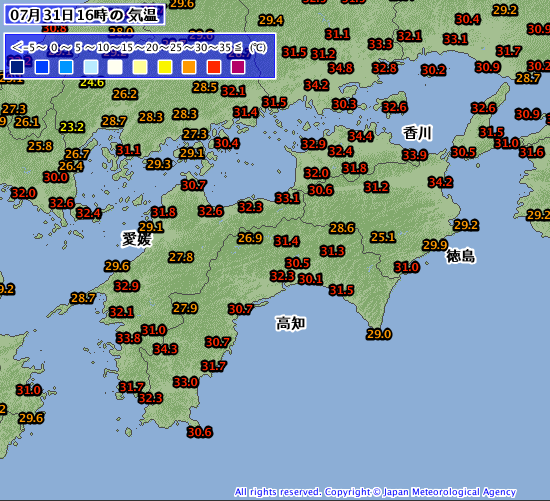
\includegraphics[width=5.5cm]{picture/vecterana1}
  \end{center}
 \caption{高知県周辺の気温(気象庁ホームページより)}
 \label{fig:ondo}
\end{minipage}
\begin{minipage}{0.5\hsize}
  \begin{center}
   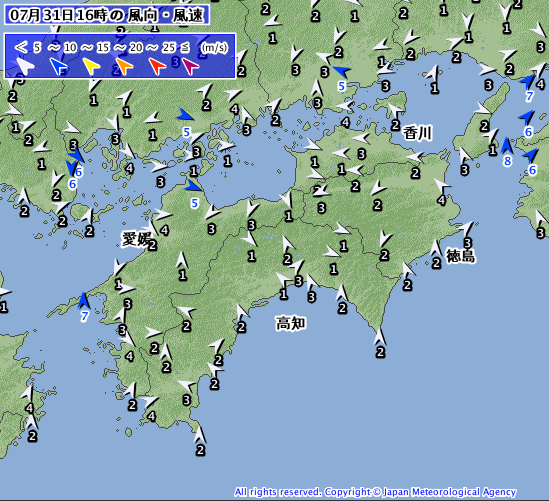
\includegraphics[width=5.5cm]{picture/vecterana2}
  \end{center}
 \caption{高知県周辺の風向と風速(気象庁ホームページより)}
 \label{fig:husoku}
\end{minipage}
\end{figure} 
ちょっと小さくて図が見えにくいかもしれないが,
天気予報とかでよく出てくる図である.
図\ref{fig:ondo}が位置に対してそこの気温というスカラー量
が決まっているような対応関係を表している図であり,
図\ref{fig:husoku}が位置に対して風向と風速というベクトル量が
決まっているような対応関係を表している図である.
すなわち,図\ref{fig:ondo}がスカラー場,図\ref{fig:husoku}が
ベクトル場を表しているような図であるというわけだ.
本来ベクトルの大きさというのは,矢印の長さで表すのが普通であるが,
図\ref{fig:husoku}は風速を矢印の色で表している.
数学や物理学のルールはその分野でもっとも便利になるように作られているので,
それ以外ではそのルールに従う必要はないのである.

ちょっと話が長くなったが,これからやるのはベクトル場やスカラー場を微分積分学の手法を用いて調べていくことである.

\section{ベクトルの微分}
まずは微分からやってみよう.$n$次元の数ベクトル$\bm{A}$があるスカラー量$t$の関数$\bm{A}(t)$だったとする.
これはつまり,$\bm{A}(t)$の各成分が$t$の関数であるということである.
\begin{eqnarray}
\bm{A}(t) = \left[
\begin{array}{c}
 A_1 (t) \\
 A_2 (t) \\
 \vdots \\
 A_n (t)
 \end{array}
\right]
\label{eq:vect}
\end{eqnarray}

$t$が微小量$\mathrm{d}t$だけ変化したとき,$\bm{A}(t)$がどれだけ変化をするかを求めたい.
微分法を使う動機はそのようなものだった.
$\bm{A}(t)$の変化$\mathrm{d} \bm{A}(t)$は
$$
\mathrm{d} \bm{A}(t) = \bm{A} (t+ \mathrm{d} t) - \bm{A} (t)
$$
である.成分表示すれば
\begin{eqnarray*}
\mathrm{d} \bm{A}(t) & = &\bm{A} (t+ \mathrm{d} t) - \bm{A} (t) \\
& = & \left[
\begin{array}{c}
A_1 (t+ \mathrm{d} t) \\
A_2 (t+ \mathrm{d} t) \\
\vdots \\
A_n (t+ \mathrm{d} t) 
\end{array}
\right]
- 
\left[
\begin{array}{c}
 A_1 (t) \\
 A_2 (t) \\
 \vdots \\
 A_n (t)
 \end{array}
\right] \\
& = &  
 \left[
\begin{array}{c}
A_1 (t+ \mathrm{d} t) - A_1 (t)\\
A_2 (t+ \mathrm{d} t) - A_2(t) \\
\vdots \\
A_n (t+ \mathrm{d} t) - A_n (t)
\end{array}
\right] \\
& = & \left[
\begin{array}{c}
 \mathrm{d} A_1 \\
 \mathrm{d} A_2 \\
 \vdots \\
 \mathrm{d} A_n
 \end{array}
\right]
\end{eqnarray*}
となる.もう見えてきただろう.
``ベクトル$\bm{A}(t)$を変数$t$で微分する''というのは$\bm{A}(t)$の変化$\mathrm{d}\bm{A}(t)$と
$t$の変化$\mathrm{d}t$の比を求めることであった.
\renewcommand{\arraystretch}{2}
\begin{eqnarray}
\frac{\mathrm{d}\bm{A}(t)}{\mathrm{d}t} = \left[
\begin{array}{c}
\displaystyle 
\frac{\mathrm{d} A_1}{\mathrm{d}t} \\
\displaystyle
\frac{\mathrm{d} A_2}{\mathrm{d}t} \\
\vdots \\
\displaystyle
\frac{\mathrm{d} A_n}{\mathrm{d}t} 
\end{array}
\right]
\label{eq:vectbibun}
\end{eqnarray}
となるのである.
つまり,ベクトルをスカラーで微分するときは,そのベクトルの各成分を微分すればよいのである.
各成分の微分は通常の微分である.簡単だろ? たったこれだけである.

\subsection{ベクトルの偏微分}
次はベクトル$\bm{A}$が複数のスカラー量の関数である場合を考えよう.とりあえず3変数の関数
$\bm{A}(x, \, y, \, z)$について考える.
これはつまり,$\bm{A}(x, \, y, \, z)$の各成分が$x, \, y, \, z$の関数であるということであった.
\renewcommand{\arraystretch}{1}
\begin{eqnarray}
\bm{A}(x, \, y, \, z) = \left[
\begin{array}{c}
 A_1 (x, \, y, \, z) \\
 A_2 (x, \, y, \, z) \\
 \vdots \\
 A_n (x, \, y, \, z)
 \end{array}
\right]
\label{eq:vecxyz}
\end{eqnarray}
多変数関数では偏微分を使うのであった.やることはさっきと同じである.
$\bm{A}(x, \, y, \, z)$を$x$で偏微分したいときは
\renewcommand{\arraystretch}{2}
\begin{eqnarray}
\frac{\partial \bm{A}}{\partial x} = \left[
\begin{array}{c}
\displaystyle 
\frac{\partial A_1}{\partial x} \\
\displaystyle
\frac{\partial A_2}{\partial x} \\
\vdots \\
\displaystyle
\frac{\partial A_n}{\partial x} 
\end{array}
\right]
\label{eq:vecxhenbibun}
\end{eqnarray}
という計算をしてやればよい.他の変数についても同様である.いちいち書かなくてもいいだろう.
\subsubsection{略記法で簡便に}
物理で使われるベクトルは,たいていは位置を表す$x, \, y, \, z$と時間$t$の4変数関数である.
これを毎回毎回$\bm{A}(x, \, y, \, z, \, t)$と書くのはさすがに面倒である.略記して表記を簡単にしてしまおう.

$x, \, y, \, z$は空間内の位置を表す.$x, \, y, \, z$をすべて決めると1つの座標$(x, \, y, \, z)$が決まるのである.
これは,たった1つのベクトルで表すことができるのだった.
$$
\bm{r} = \left[
\renewcommand{\arraystretch}{1}
\begin{array}{c}
x \\
y \\
z
\end{array}
\right]
$$
とベクトル$\bm{r}$を定めれば,$x, \, y, \, z$をすべて決めるのとベクトル$\bm{r}$を決めるのはまったく同じことである.
このベクトル$\bm{r}$は位置を表すことから,$\bm{r}$は位置ベクトル,もしくは単に位置と呼ばれるのであった.
つまり,$4$変数のベクトル$\bm{A}(x, \, y, \, z, \, t)$は,位置ベクトル$\bm{r}$を用いることで,
あたかも$2$変数のベクトル$\bm{A}(\bm{r}, \, t)$であるかのように考えることができるのである.
\footnote{数学では普通記号を変えて$\bm{A}'(\bm{r}, \, t)$などというように区別するのだが,
物理学では記号を変えることはほとんどない.
理由は各自考えてもらいたい.}
もちろんこれはベクトルに限った話ではない.
関数$f(x, \, y, \, z, \, t)$は$f(\bm{r}, \, t)$と略記できる.
形式的には4次元の数ベクトルを使って時間$t$もベクトルの中に入れてしまうこともできるのだが,
意味を考えればそうはしない方がいいだろう.$\bm{r}$に位置
という解釈を付け加えることができるのだ.
$\bm{A}(\bm{r}, \, t)$は位置と時間に依存するベクトルであるということである.

こう見ると,$\bm{A} (\bm{r} , \, t)$が位置と時間のペアの関数であるが,
やはりこれもベクトル場と呼ばれる.
$\bm{A} (\bm{r} , \, t)$は時刻に依存して
無限個のベクトル場を対応させるような関数だと考えられるからだ.
``時間に依存するベクトル場''とでも呼んでおけばなんとなくカッコイイ気がするだろう.

\subsection{ベクトルをベクトルで微分する}
``ベクトルに依存するベクトル''というものが出てきた.とりあえずそのベクトルを$\bm{A}(\bm{r}, \, t)$としておこう.
$\bm{r}$を微小量$\mathrm{d}\bm{r}$だけ変化させたとき,$\bm{A}(\bm{r}, \, t)$がどれくらい変化するかを調べてみよう.

$\bm{r}$が変化するというのは$x, \, y, \, z$が変化するというのに他ならない.
このときの$\bm{A}(\bm{r}, \, t)$を求めたいのだが,複数の変数が同時に変化するときには全微分という概念を使えばいいのだった.
全微分の解説をしたときにはベクトルではなかったが,ベクトルでも同じようなことが言えるのは容易に想像がつくだろう.
$\bm{A}(\bm{r}, \, t)$は$x, \, y, \, z, \, t$の4つの変数からなる関数であるが,
いまは$t$が変化しないという想定なので$\mathrm{d}t = 0$である.よって$\bm{A}(\bm{r}, \, t)$の全微分$\mathrm{d}\bm{A}$は
$$
\mathrm{d}\bm{A} =
\frac{\partial \bm{A}}{\partial x} \mathrm{d}x + \frac{\partial \bm{A}}{\partial y} \mathrm{d}y + 
\frac{\partial \bm{A}}{\partial z} \mathrm{d}z
$$
となる.ベクトルを偏微分するというのは各成分を偏微分するということであった.
結局のところ,全微分も各成分の全微分をとればいいのである.
$$
\mathrm{d}\bm{A} = \left[
\renewcommand{\arraystretch}{1}
\begin{array}{c}
 \mathrm{d} A_x \\
 \mathrm{d} A_y \\
 \mathrm{d} A_z
 \end{array}
 \right]
$$
あとは$\mathrm{d}\bm{A}$と$\mathrm{d}\bm{r}$の比をとるだけなのだが,ここで問題が生じる.
$\mathrm{d}\bm{r}$はベクトルであった.しかし,ベクトルで割るなどという演算は定義してはいない.
だがとりあえずそういうものを考えてみることにする.
$$
\mathrm{d}\bm{r} = \left[
\renewcommand{\arraystretch}{1}
\begin{array}{c}
 \mathrm{d} x \\
 \mathrm{d} y \\
 \mathrm{d} z
 \end{array}
 \right]
$$
であるから,とりあえず
\begin{eqnarray}
\frac{\partial \bm{A}}{\partial \bm{r}} = \left[
\renewcommand{\arraystretch}{2}
\begin{array}{c}
\displaystyle
\frac{\partial A_x (x, \, y, \, z, \, t)}{\partial x} \\
\displaystyle
\frac{\partial A_y (x, \, y, \, z, \, t)}{\partial y} \\
\displaystyle
\frac{\partial A_z (x, \, y, \, z, \, t)}{\partial z}
\end{array}
\right]
\label{eq:vecvecbibun}
\end{eqnarray}
と定義してみてはどうだろうか.``$\mathrm{d}$''が``$\partial$''になっているのは表記上の都合である.
いまは時間の変化は気にせず位置の変化のみを考えているのだった.
注意しなければならないのは,いまベクトルの割り算のような形式で書いたが,
一般にベクトルの割り算というものを定義したのではなく,
ベクトルの微分というものを考えるうえでの都合でとりあえず導入した書き方にすぎないということだ.
さらに気を付けなくてはならないのは,添え字についている$x$と変数の$x$は別物であるということだ.
$A_x$と書いてあるところの添え字の$x$は``$\bm{A}$の$x$成分''という意味での$x$である.
$A_x (x, \, y, \, z, \, t)$は$x, \, y, \, z, \, t$を変数とする4変数関数であった.他の成分も同じだ.
ここまで言えばわかるだろう.あとは自分で考えてほしい.

とにかく式(\ref{eq:vecvecbibun})のような表現方法は
何かしっかりした根拠があって導入されたものではなく,とりあえず導入されたものにすぎないようである.
とはいえ,誤解なくきちんと使えばいろいろと面白い性質が導けたりするのだが,とりあえず本書ではそういうところには立ち入らないことにする.

いろいろ書いたが,ベクトルの微分というのは結局普通の関数の微分とほとんど変わらないのである.



\section{線素ベクトルと面素ベクトル}
\subsection{曲線の接ベクトルと法線ベクトル}
微分積分学の復習をしたときに,``微分係数は接線の傾きである''という話をしたのであった.
これからの議論を円滑に進めるために,この話をもう少し掘り下げておかねばならない.

空間に存在する曲線$C$を考える.簡単のため,$C$をパラメータ表示して
\begin{align*}
x & = \varphi (t) \\
y & = \psi (t) \\
z & = \xi (t)
\end{align*}
と表しておこう.
あるいは$C$の各点を表す位置ベクトル$\bm{r}$が$t$の関数であると考えてもいい.
そのような関数を$\bm{r} (t)$と表そう.
こちらの方が表現が簡単なので,今後はこちらの表現を用いることにする.
ついでに$\varphi, \, \psi , \, \xi$という記号も使うのをやめて
\begin{align}
\renewcommand{\arraystretch}{1}
\bm{r} (t) = \left[
\begin{array}{c}
x(t) \\
y(t) \\
z(t)
\end{array}
\right]
\label{eq:curvert}
\end{align}
と書き表しておこう.
式(\ref{eq:curvert})が$C$のパラメータ表示だと思うことにするのだ.

\subsubsection{接ベクトル}
$C$上に2点P, Qをとる.
Pを表す位置ベクトルは$\bm{r}(t)$で,
Qを表す位置ベクトルは$\bm{r} (t + \varDelta t)$であるとしておこう.
そうすると,
\begin{align*}
\overrightarrow{\mathrm{PQ}} = \bm{r} (t + \varDelta t) - \bm{r} (t) = \varDelta \bm{r} (t)
\end{align*}
となる.ただし,$\varDelta \bm{r} (t)$は$\varDelta t$に対する$\bm{r}(t)$の変分である.
この量を$\varDelta t$で割り,$\varDelta t$を0に限りなく近づけていく.
このとき,QはPに限りなく近づいていくことになる.
こうして得られるベクトルは,要するに$\bm{r}$を$t$で微分して得られるベクトルである.
\begin{align}
\frac{\mathrm{d} \bm{r}(t) } {\mathrm{d} t} = \left[
\renewcommand{\arraystretch}{2}
\begin{array}{c} 
\displaystyle \frac{ \mathrm{d} x} { \mathrm{d} t} \\
\displaystyle \frac{ \mathrm{d} y} { \mathrm{d} t} \\
\displaystyle \frac{ \mathrm{d} z} { \mathrm{d} t} 
\end{array}
\right]
\end{align}
というベクトルが得られた.
表記を簡単にするため,このベクトルを$\dot{\bm{r}}(t)$と表しておく.
このベクトル$\dot{\bm{r}}(t)$を$C$の点Pにおける\emph{接ベクトル},
\index[widx]{せつべくとる@接ベクトル}
もしくは\emph{接線ベクトル}\index[widx]{せっせんべくとる@接線ベクトル|see{接ベクトル}}と呼ぶ.

$\overrightarrow{\mathrm{PQ}}$はPとQを結ぶベクトルである.
QをPに限りなく近づける極限を考えれば,
$\overrightarrow{\mathrm{PQ}}$は$C$に接すると考えても問題ないということになる.

\begin{figure}[h]
 \begin{center}
 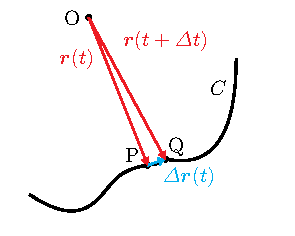
\includegraphics[width=5cm]{picture/vecterana3}
 \caption{接ベクトル}
\label{fig:setuvec}
 \end{center}
\end{figure}

さらにこのベクトルの大きさを1に調整する.それを$\bm{t}$と表すことにすると,
\begin{align}
\bm{t} = \frac { \dot{ \bm{r} } (t) } { \lvert \dot{ \bm{r} } (t) \rvert }
\end{align}
というベクトルが得られる.
$\bm{t}$の大きさは1で,$\dot{\bm{r}}(t)$と同じ方向を向いたベクトルである.
$\bm{t}$を$C$の点Pおける\emph{単位接ベクトル},\index[widx]{せつべくとる@接ベクトル!たんい@単位---}
もしくは\emph{単位接線ベクトル}\index[widx]{せっせんべくとる@接線ベクトル!たんい@単位---|see{単位接ベクトル}}
と呼ぶ.
$\bm{t}$は接線(tangent)の頭文字をとって$\bm{t}$と書いている.
パラメータを表す$t$と被ってしまっているが,ベクトルとスカラーをきちんと使い分ければ
混乱することもないだろう.

$\bm{t}$はパラメータ$t$が微小変化したときの$\bm{r}(t)$の変化の向きを表すベクトルである.
1変数関数におけるグラフの接線と同じように考えれば,
$\bm{t}$は点Pにおいて$C$と接するといえるだろう.

\subsubsection{弧長パラメータ}
さっきまでの話では,パラメータ$t$に対しては何の意味も与えていなかった.
しかし,このパラメータに弧長という意味付けをしてやることにより,
いろいろと便利なことがある.
その話を少ししておこう.

曲線$C$をパラメータ$t$を用いてパラメータ表示して,
$C$上の各点を$\bm{r}(t)$とおく.$C$上に定点$\bm{r}(t_0)$をとり,その点から別の点$\bm{r}(t)$までの
$C$に沿って測った曲線の長さを$s$とおく.
$s$はよく知られているように,
\begin{align}
s = \int _{t_0}^t \lvert \dot{ \bm{r} } (t) \rvert \, \mathrm{d} t
\label{eq:kotyou1} 
\end{align}
と表せる.ちょっとなじみがないという人も
\begin{align}
s = \bigintsss _{t_0}^t \sqrt{ \left( \frac{ \mathrm{d} x }{\mathrm{d} t} \right)^2
+ \left( \frac{ \mathrm{d} y } {\mathrm{d} t} \right)^2 
+ \left( \frac{ \mathrm{d} z } {\mathrm{d} t} \right)^2}  \, \mathrm{d} t
\label{eq:kotyou2} 
\end{align}
と書かれれば納得できるだろう.導出は高校レベルである.
あらためてここでやる必要もあるまい.
この$s$を$C$の点$\bm{r}(t_0)$から点$\bm{r}(t)$までの
\emph{弧長}\index[widx]{こちょう@弧長}と呼ぶ.

$s$と$t$は1対1に対応している.
つまり,$s$の値が決まるとそれに対応するような$t$はただ1つに定まる.
$t$が定まれば$C$上の1点が決まるので,
結局$s$と$C$上の点が1対1に対応していることになる.
すなわち,$s$を$C$を表現するためのパラメータとして採用できるということになる.
曲線$C$を弧長$s$でパラメータ表示したとき,
$s$を\emph{弧長パラメータ}\index[widx]{ぱらめーた@パラメータ!こちょう@弧長---}と呼ぶ.
弧長パラメータを用いるといろいろと便利なことがある.
それを今から見ていこう.

弧長パラメータ$s$を用いたときの$C$の接ベクトルを考えてみよう.
$C$上の各点$\bm{r}(s)$について,
\begin{align*}
\frac{\mathrm{d} \bm{r} (s) }{\mathrm{d} s} = \left[
\begin{array}{c} 
\displaystyle \frac{ \mathrm{d} x }{\mathrm{d}s} \\
\displaystyle \frac{ \mathrm{d} y }{\mathrm{d}s} \\
\displaystyle \frac{ \mathrm{d} z }{\mathrm{d}s} 
\end{array}
\right]
\end{align*}
であるが,これを単に$\bm{r}'(s)$と書き表す.
パラメータが$t$と表された場合には微分を$\dot{ \bm{r} } (t)$と書いたが,
慣例として,弧長パラメータ$s$を用いたときにはこれを$\bm{r}'(s)$と書き表す.
これは慣習的なものだが,慣れてくるとなかなか便利だったりする.

さて,$\bm{r}'(s)$の大きさを考えてみる.式(\ref{eq:kotyou1})と微分積分学の基本定理により
\begin{align*}
 \frac{\mathrm{d} s}{\mathrm{d} s} = \lvert \bm{r}'(s) \rvert 
\end{align*}
である.式(\ref{eq:kotyou1})はパラメータがどんなものであっても成り立つのであったから,
当然弧長パラメータを採用したときでも成り立つべきである.
これにより,
\begin{align*}
\lvert \bm{r}'(s) \rvert = 1
\end{align*} 
を得る.パラメータとして弧長パラメータを採用した場合には,
接ベクトルと単位接ベクトルが一致するのである.
イメージもしやすいし,計算も簡便になるといいことだらけである.
そういうわけで,パラメータとして弧長パラメータを採用することはこれからたくさんあるだろう.

\subsubsection{法線ベクトルと曲率}
さっき求めた曲線の単位接ベクトルの大きさは1である.
いま,パラメータ表示された曲線$C$の点Pにおける単位接ベクトル$\bm{t}$を考えると,
\begin{align*}
\bm{t} \cdot \bm{t} =1
\end{align*}
が成り立つ.この式の両辺をパラメータ$t$で微分してやる.
\begin{align*}
\frac{ \mathrm{d} } {\mathrm{d} t} ( \bm{t} \cdot \bm{t} ) =0
\end{align*}
説明してなかったが,内積についても積の微分公式と同じような公式が成り立っている.
\begin{align}
\frac{ \mathrm{d} } {\mathrm{d} t } (\bm{A} \cdot \bm{B} ) 
= \frac{ \mathrm{d} \bm{A} } { \mathrm{d} t} \cdot \bm{B}
+ \bm{A} \cdot \frac{ \mathrm{d} \bm{B} } { \mathrm{d} t } 
\label{eq:vecsekibibun}
\end{align} 
関数の``積''がベクトルの``内積''に変わっただけで,ほぼ同じ形をしている.
同様の公式が外積やスカラー関数倍に関しても成り立っているのだが,いちいち書く必要もないだろう.
とにかく,式(\ref{eq:vecsekibibun})を用いれば,
\begin{align*}
\frac{ \mathrm{d} \bm{t} } {\mathrm{d} t} \cdot \bm{t} 
+ \bm{t} \cdot \frac{ \mathrm{d} \bm{t} } {\mathrm{d} t} & = 0 \\
\therefore \bm{t} \cdot \frac{ \mathrm{d} \bm{t} } {\mathrm{d} t } & = 0
\end{align*}
となる.内積は順番を変えても結果が変わらないことを用いた.
ベクトルの内積が0ということは,
そのベクトルが直交するということであった.
すなわち,$\bm{t}$の微分$\dot{ \bm{t} }$は$\bm{t}$と直交することになる.
$\bm{t}$は$C$の接線方向のベクトルである.
接線と直交するような直線を\emph{法線}\index[widx]{ほうせん@法線}と呼ぶのであった.
そういうわけで,$\dot { \bm{t} }$を$C$の点Pにおける
\emph{主法線ベクトル}\index[widx]{しゅほうせんべくとる@主法線ベクトル}と呼ぶ.
なぜ法線ベクトルでなく主法線ベクトルと書いているかというと,
いま,3次元空間で考えていて,接線に直交するといってもいろいろな方向があるからだ.
その中でも使いやすい特定の方向のベクトルを抽出して使っているので,
これを主法線ベクトルと呼ぶわけだ.
このベクトルの大きさは1とは限らない.パラメータとして弧長パラメータを用いても無理そうである.
そこで,主法線ベクトルの大きさを1に調整したベクトルを$\bm{n}$と書いて,
\emph{単位主法線ベクトル}\index[widx]{しゅほうせんべくとる@主法線ベクトル!たんい@単位---}と名付けよう.
\begin{align}
\bm{n} = \frac{ \dot{ \bm{t} } } { \lvert \dot { \bm{t} } \rvert}
\label{eq:syuhousen}
\end{align}
ということである.

ここからは,パラメータとして弧長パラメータを採用した場合について考える.
$C$の点Pにおける主法線ベクトル$\bm{t}'$は,$\bm{t}$
の弧長パラメータに対する変化率を表す.
$\bm{t}$の大きさは常に1なので,$\bm{t}'$は実質的には$\bm{t}$
の向きの変化を表していることになるだろう.
これはすなわち,$C$がどのくらい曲がっているかを表す量である.
$\bm{t}'$の大きさ$\lvert \bm{t}' \rvert$を
$C$の点Pにおける\emph{曲率}\index[widx]{きょくりつ@曲率}といい,
$\kappa$で表す.
また,$\kappa$の逆数を$C$の点Pにおける
\emph{曲率半径}\index[widx]{きょくりつ@曲率!はんけい@---半径}といい,
$\rho$と表す.
すなわち,
\begin{align}
\bm{t}' = \kappa \bm{n} = \frac{1}{\rho} \bm{n}
\label{eq:kyokuritu}
\end{align}
である.細かい話は抜きにして結果だけ言えば,点Pにおける$C$の曲率半径$\rho$は
点Pにおいて$C$に接するような円を考えたとき,その円の半径を表すものになっている.
これはパラメータとして弧長パラメータを採用したための結果である.

\subsubsection{従法線ベクトル}
さて,$\bm{t}$と$\bm{n}$の外積を考え,これを$\bm{b}$とおく.
\begin{align}
\bm{b} = \bm{t} \times \bm{n} 
\label{eq:juhousen}
\end{align}
$\bm{b}$は$\bm{t}$にも$\bm{n}$にも直交するベクトルであり,
従って$\bm{b}$も法線方向を向いたベクトルである.
さらに,$\bm{t}$と$\bm{n}$は単位ベクトルで,直交するのであった.
よって$\bm{b}$も単位ベクトルである.
このベクトル
$\bm{b}$を\emph{単位従法線ベクトル}\index[widx]{たんいじゅうほうせん@単位従法線ベクトル}という.

\subsubsection{線素ベクトル}
ここからが本題である.
曲線$C$を弧長パラメータを用いてパラメータ表示して,これを$\bm{r} (s)$とする.
$C$上に点Pを任意にとり,Pにおける$C$の単位接ベクトル$\bm{t}$を考える.
弧長パラメータ$s$を$\mathrm{d} s$だけ変化させたとき,この$\mathrm{d}s$を
点Pにおける$C$の\emph{線素}\index[widx]{せんそ@線素}と呼び,
$\bm{r}(s)$の変化$\mathrm{d} \bm{r}$を$C$の点Pにおける
\emph{線素ベクトル}\index[widx]{せんそ@線素!べくとる@---ベクトル}と呼ぶ.
線素ベクトルは,通常$\mathrm{d} \bm{s}$と書き表すことが多い.
弧長パラメータの変化に向きを付与したようなイメージである.
というのも,
\begin{align*}
\mathrm{d} \bm{r} = \frac{ \mathrm{d} \bm{r} } { \mathrm{d} s} \mathrm{d} s
\end{align*}
であり,弧長パラメータを採用しているときには接ベクトルがそのまま単位接ベクトルとなるのだから
\begin{align*}
\mathrm{d} \bm{r} = \bm{t} \, \mathrm{d} s
\end{align*}
ということになるからだ.
従って,$\mathrm{d} \bm{r}$は$\bm{t}$と同じ向きで,大きさ$\mathrm{d} s$
のベクトルだから,これを
\begin{align}
\mathrm{d} \bm{s} = \bm{t} \, \mathrm{d} s
\label{eq:sensovec}
\end{align}
と表すことにそれほど抵抗はないだろう.

線素と線素ベクトルは,これから場の積分論を展開していくうえで中心的な役割を果たす.

\subsection{曲面の法線ベクトルと面素ベクトル}

これからは空間に存在する曲面$S$について考える.
曲線のときと大体同じ話が続くので,パパっと進むことにしよう.
$S$はパラメータを2種類使ってパラメータ表示できる.
$S$上の各点$\bm{r}$をパラメータ$u, \, v$を用いてパラメータ表示して,
$\bm{r}(u, \, v)$と表すことにする.

\subsubsection{接平面}
パラメータ$u, \, v$はそれぞれ勝手に動くのだが,とりあえず$u$の値を
ある定数$u_0$に固定してみる.そうすると,ベクトル$\bm{r}(u_0, \, v)$
は,あたかも1つのパラメータによってパラメータ表示されるような図形であるとみなすことができる.
パラメータ1つでパラメータ表示されるような図形というのは曲線のことであったから,
この曲線を$S$上の\emph{$v$曲線}と呼ぶことにしよう.
実際には,$u$をどんな値に固定するかによって無限に多くの曲線が得られるわけだが,
それらを全部まとめて$v$曲線と呼ぶのである.
同様にして,$v$を定数$v_0$と固定して$u$を動かしたときに$\bm{r}(u, \, v_0)$
の軌跡として得られる曲線を$S$上の\emph{$u$曲線}と呼ぶ.

曲線があれば接線を考えることができる.
いま,パラメータ表示された曲面$S$上に点Pをとり,その位置ベクトルを$\bm{r}(u, \, v)$とする.
その$u$曲線上の接ベクトルを考えると,これは$\bm{r}(u, \, v)$を
$u$で微分して得られるベクトルであるが,
$v$を定数だと思っているということを考えれば,偏微分を使うべきである.
すなわち,
\begin{align*}
\frac{ \partial \bm{r} } {\partial u} 
\end{align*}
は$S$上の$u$曲線の点Pにおける接ベクトルであるということだ.
略記して,
\begin{align*}
\frac{ \partial \bm{r} } {\partial u} = \bm{r}_u
\end{align*}
と表そう.下付きの添え字で偏導関数を表すというのは以前説明したことである.
同様にして,
\begin{align*}
\frac{ \partial \bm{r} } {\partial v} = \bm{r}_v
\end{align*}
は$S$上の$v$曲線の点Pにおける接ベクトルであることもわかるだろう.

さて,$S$上の点Pにおいて,点Pで接するような2本のベクトル$\bm{r}_u, \, \bm{r}_v$
が得られた.この2本のベクトルは線形独立であると考えていいだろう.
このとき,$\bm{r}_u$と$\bm{r}_v$が貼る平面を
$S$の点Pにおける\emph{接平面}\index[widx]{せつへいめん@接平面}という.

\subsubsection{法線ベクトルと曲面の面積}
さっきの話からも明らかなように,$\bm{r}_u$と$\bm{r}_v$の外積を考えれば,
これは点Pにおける$S$の接平面に垂直なベクトルとなる.
このベクトルを$S$の点Pにおける\emph{法線ベクトル}\index{ほうせんべくとる@法線ベクトル}と呼ぶ.
さらに,法線ベクトルの大きさを1に調整して得られるベクトルを
$S$の点Pにおける\emph{単位法線ベクトル}\index[widx]{ほうせんべくとる@法線ベクトル!たんい@単位---}といい,
これは曲線のときと同じく$\bm{n}$という記号で表す.$\bm{n}$は
\begin{align}
\bm{n} = \frac{ \bm{r}_u \times \bm{r}_v } { \lvert \bm{r}_u \times \bm{r}_v \rvert }
\label{eq:kyokumenhou}
\end{align}
と表されるベクトルである.

\begin{figure}[h]
 \begin{center}
 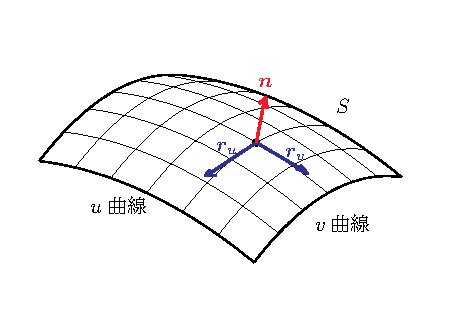
\includegraphics[width=8cm]{picture/vecterana4}
 \caption{曲面の法線ベクトル}
\label{fig:kyokuhousen}
 \end{center}
\end{figure}

ここから曲面$S$の面積を計算することができる.
パラメータ$u, \, v$がそれぞれ$\mathrm{d} u, \, \mathrm{d}v$だけ微小変化したとき,
その変化に対して点Pを表すベクトル$\bm{r}(u, \, v)$が変化し得る領域は,
4点$\bm{r}(u, \, v), \, \bm{r}(u + \mathrm{d}u, \, v), \, 
\bm{r} (u+ \mathrm{d}u, \, v+\mathrm{d}v), \, \bm{r} (u, \, v +\mathrm{d}v )$
を結んだ四角形である.
これらの位置ベクトルは偏微分や全微分の知識を駆使して
\begin{align*}
\bm{r} (u + \mathrm{d} u, \, v) & = \bm{r}(u, \, v) + \bm{r}_u \, \mathrm{d} u \\
\bm{r} ( u + \mathrm{d} u, \, v + \mathrm{d} v) & = 
\bm{r} (u, \, v)+ \bm{r}_u \, \mathrm{d} u + \bm{r}_v \, \mathrm{d} v \\ 
\bm{r} (u, \, v + \mathrm{d} v) & = \bm{r}(u, \, v) + \bm{r}_v \, \mathrm{d}v 
\end{align*}
と求められる.結局のところ,この四角形は
2つのベクトル$\bm{r}_u \, \mathrm{d}u, \, \bm{r}_v \, \mathrm{d}v$が貼る平行四辺形であって,
その面積$\mathrm{d}S$は外積を用いて
\begin{align}
\mathrm{d} S = \lvert \bm{r}_u \times \bm{r}_v \rvert \, \mathrm{d} u \mathrm{d}v
\label{eq:menso}
\end{align}
と表せる.
この$\mathrm{d}S$を点Pにおける$S$の\emph{面素}\index[widx]{めんそ@面素}
もしくは\emph{面積素}\index[widx]{めんせきそ@面積素|see{面素}}と呼ぶ.
$\mathrm{d}S$を$S$全体にわたって足し合わせれば,曲面$S$の面積が求められる.
\begin{align}
S = \iint_S \lvert \bm{r}_u \times \bm{r}_v \rvert \, \mathrm{d} u \mathrm{d} v
\label{eq:kyokumenseki}
\end{align}
これが曲面の面積公式である.
この式はヤコビアンでも表せて,
\begin{align}
S = \bigintsss \! \! \! \! \! \bigintsss_S 
{ \sqrt{ \left( \frac{ \partial ( x, \, y) } {\partial (u, \, v) } \right) ^2
+ \left( \frac{ \partial ( y, \, z) } {\partial (u, \, v) } \right) ^2
+ \left( \frac{ \partial ( z, \, x) } {\partial (u, \, v) } \right) ^2 } \, \mathrm{d}u \mathrm{d}v }
\label{eq:kyokujacobian}
\end{align}
となる.導出は読者に任せることにする.
\begin{itembox}[l]{課題}
半径$r$の球面$S_0$を
\begin{align*}
\renewcommand{\arraystretch}{1}
\bm{r} (\theta, \, \varphi) = \left[
\begin{array}{c}
r \sin \theta \cos \varphi \\
r \sin \theta \sin \varphi \\
r \cos \theta
\end{array}
\right]
\end{align*}
とパラメータ表示する.累次積分を使い,
$\theta$と$\varphi$がそれぞれ独立に
$0 \leq \theta \leq \pi , \, - \pi \leq \varphi \leq \pi$
の範囲を動くときの$S_0$の面積が$4 \pi r^2$になることを確かめよ.

また,3つのベクトル$\dfrac{ \bm{r}_{\theta} }{\lvert \bm{r}_{\theta} \rvert } , \,
\dfrac{ \bm{r}_{\varphi} }{\lvert \bm{r}_{\varphi} \rvert}, \, 
\dfrac{ \bm{r}_{\theta} }{\lvert \bm{r}_{\theta} \rvert} 
\times \dfrac{ \bm{r}_{\varphi} }{\lvert \bm{r}_{\varphi} \rvert} $を求め,$[ \, \cdot \, ]$
を用いた成分表示の形式ではなく
$\bm{e}_x, \, \bm{e}_y , \bm{e}_z$の線形結合の形式で表せ.

以上の計算で得られた3つのベクトルと,$\bm{r}(\theta , \, \varphi)$の
成分中にある$r$を変数とみなし,$\bm{r}(\theta , \, \varphi)$を
$r$で偏微分し,大きさを1に調整することで得られる
$\dfrac{\bm{r}_r}{\lvert \bm{r}_r \rvert}$というベクトル
を眺め,どんなベクトルか,そしてなぜそのような計算結果になったかを考察せよ.
\end{itembox}

\subsubsection{面素ベクトル}
曲面$S$について,$S$上の点Pを任意にとり,その点の位置ベクトルを$\bm{r}(u, \, v)$とおく.
大きさが点Pにおける$S$の面素$\mathrm{d}S$で,
点Pにおける$S$の単位法線ベクトル$\bm{n}$と同じ向きのベクトルを
点Pにおける$S$の\emph{面素ベクトル},\index[widx]{めんそ@面素!べくとる@---ベクトル}
もしくは\emph{面積素ベクトル}\index[widx]{めんせきそ@面積素!べくとる@---ベクトル|see{面素ベクトル}}といい,
$\mathrm{d} \bm{S}$と表す.
\begin{align}
\mathrm{d} \bm{S} = \bm{n} \, \mathrm{d}S 
\label{eq:mensovec}
\end{align}

面素ベクトルは,さも曲面上に面積$\mathrm{d}S$の微小な平面を考え,
その平面の法線ベクトルを表しているようなイメージである.
面素と面素ベクトルも場の積分で活躍する量となる.

\section{場の積分}
これからやるのはベクトル場やスカラー場を積分することである.
積分には積分領域がつきものであるが,
それを一般の曲線や曲面に拡張したい.
1変数関数の積分の場合には積分領域は直線であったし,
重積分のときには積分領域は平面に限られていたのであった.
それに,ベクトル場についてはなにもしていない.
これまでの節で準備はほとんど終わっているので,
これからは実際に積分をやっていこう.

\subsection{スカラー場の線積分}

スカラー場$f(\bm{r})$と空間に存在する曲線$C$を考える.
話を簡単にするため,$C$上の各点$\bm{r}$は,弧長パラメータ$s$を用いて
$\bm{r}(s)$とパラメータ表示されているとしよう.
\subsubsection{今度は最初に厳密な定義}
曲線$C$には端点$\bm{r}(a)$から$\bm{r}(b)$があるとして,
$C$を分割することを考え,その分割を
\begin{align*}
\Delta : \bm{r}(a) = \bm{r}(s_0), \, \bm{r}(s_1), \, \bm{r}(s_2), \, \cdots , \, \bm{r}(s_n) = \bm{r}(b)
\end{align*}
とおく.そして,各分点間での$C$の弧長を
\begin{align*}
\varDelta s_i = \int _{s_{i-1} } ^{s_i} \lvert \bm{r} (s) \rvert \, \mathrm{d}s 
\end{align*}
とおく.さて,2点$\bm{r}(s_{i-1})$から$\bm{r}(s_i)$の間の
$C$上の点から1点$\bm{r}_i$を任意にとり,
その点での$f(\bm{r})$の値$f( \bm{r}_i )$と,分割幅$\varDelta s_i$
をかけて足し合わせる.これでRiemann和の出来上がりである.
\begin{align*}
\sum_{i=1}^n f(\bm{r}_i) \varDelta s_i
\end{align*}
そして,各分割幅の最大値$\delta$が限りなく小さくなるような極限
\begin{align*}
\lim _{\delta \to 0} \sum_{i=1}^n f(\bm{r}_i) \varDelta s_i
\end{align*}
を考え,この極限が分割の仕方や各点$\bm{r}_i$の取り方に依存せずに
一定の値に確定するのであれば,その値をスカラー場$f(\bm{r})$の$C$に沿った
\emph{線積分}\index[widx]{すからーば@スカラー場!のせんせきぶん@---の線積分}といい,
\begin{align*}
\int_C f(\bm{r}) \, \mathrm{d} s 
 \end{align*}
と書き表す.
1変数関数の積分とほとんど変わらない.
\subsubsection{もうちょっと簡単な定義}
さっき書いたのはきちんとした定義であるが,
実用上はもっと簡単に(そして大雑把に)考えた方が何かと便利である.

曲線$C$上に点$\bm{r}(s)$を任意にとり,
その点における線素$\mathrm{d}s$を考え,
この線素と点Pにおける$f(\bm{r})$の値との積$f(\bm{r}(s)) \, \mathrm{d} s $を,
$C$上全体にわたって足し合わせる.
これをスカラー場$f(\bm{r})$の$C$に沿った
\emph{線積分}\index[widx]{すからーば@スカラー場!のせんせきぶん@---の線積分}と呼び,
\begin{align*}
\int_C f( \bm{r} ) \, \mathrm{d}s
\end{align*}
と表す.
やっぱり普通の積分とあまり変わらない気がする.

また,もしも$C$が閉曲線であれば,$\int$記号に丸をくっつけて
$\oint$とし,$C$も閉曲線であることを強調するために$C_0$と添え字をつけて
\begin{align*}
\oint_{C_0} f( \bm{r} ) \, \mathrm{d} s
\end{align*}
と表し,スカラー場$f(\bm{r})$の閉曲線$C_0$に沿った
\emph{周回積分}\index[widx]{すからーば@スカラー場!のしゅうかいせきぶん@---の周回積分}と呼ぶ.
ただし,$\oint$記号を使うかどうかや$C_0$という表し方をするかどうか
は人によって割と差異がある.
この記法に従わない本もかなり多いので注意しよう.

\subsubsection{線積分の計算は簡単である}
線積分の実際の計算は割と簡単である.
``$C$上全体にわたって足し合わせる''というのは結局
弧長パラメータ$s$を考えている範囲全体にわたって動かして,
各点での値を足し合わせるということだから,
もし$s$が$a$から$b$まで動くのであれば,
\begin{align}
\int_C f(\bm{r} ) \, \mathrm{d}s = \int _a^b f(\bm{r} (s) ) \, \mathrm{d} s
\label{eq:sensekikeisan}
\end{align}
という計算をしてやればよいということになる.
$f(\bm{r}(s))$はただの$s$を変数とするスカラーであり,
式(\ref{eq:sensekikeisan})の右辺は$s$に関する普通の積分であるから
簡単に計算できるはずだ.

パラメータ表示は弧長パラメータによるものでなくともよい.
もし弧長パラメータとは限らないパラメータ$t$で$C$がパラメータ表示されていたならば,
まず$C$の線素$\mathrm{d}s$を
\begin{align}
\mathrm{d} s = \lvert \dot {\bm{r} } (t) \rvert  \, \mathrm{d} t
\label{eq:sensopara}
\end{align}
によって求めてから,
\begin{align}
\int_C f(\bm{r} ) \, \mathrm{d} s 
= \int_{t_0}^{t_1} f(\bm{r}(t) )\lvert \dot{ \bm{r} } (t) \rvert \, \mathrm{d} t
\label{eq:sensekibunpara}
\end{align}
という計算をしてやることになる.
$t_0$や$t_1$というのは$C$の端点に対応するパラメータの値であるとした.

線積分を考えるとき,
積分領域となった曲線$C$のことを
\emph{積分経路},\index[widx]{せきぶんけいろ@積分経路}
もしくは単に\emph{経路}\index[widx]{けいろ@経路|see{積分経路}}などと呼ぶ.
また,$C$の端点$\bm{r}(t_0)$と$\bm{r}(t_1)$のことを
それぞれ$C$の\emph{始点}\index[widx]{せきぶんけいろ@積分経路!のしてん@---の始点},
および$C$の\emph{終点}\index[widx]{せきぶんけいろ@積分経路!のしゅうてん@---の終点}という.

\subsubsection{線積分には向きがある}
$C$上全体にわたって足し合わせると書いたが,
そのイメージはパラメータ$t$を$t_0$から$t_1$まで増加させるようなイメージであった.
このパラメータ変化の向きを逆にしたらどうなるだろう? これは,
\begin{align*}
\int_{t_1}^{t_0} f(\bm{r}(t)) \lvert \dot { \bm{r} } (t)  \rvert \, \mathrm{d} t
\end{align*}
という積分を考えることに相当するので,
\begin{align*}
\int_{t_1}^{t_0} f(\bm{r}(t)) \lvert \dot { \bm{r} } (t)  \rvert \, \mathrm{d} t
= - \int_{t_0}^{t_1} f(\bm{r}(t)) \lvert \dot { \bm{r} } (t)  \rvert \, \mathrm{d} t
\end{align*}
ということになる.
どちらも$C$上全体にわたっての和を表しているのに,値が正負逆転していることになってしまう.
これは,``パラメータ変化の向き''によって自然と曲線に向きが付与されたことによるものである.
$C$の端点を始点,終点というように呼んだが,
これは$C$に向きがあるようにイメージしてのことだったのである.

一般に,経路$C$が与えられたとき,
$C$の始点と終点を入れ替えたような経路を$-C$と書き表す.
この書き方は,
\begin{align}
\int_{-C} f( \bm{r} ) \, \mathrm{d} s = - \int_C f( \bm{r} ) \, \mathrm{d}s 
\label{eq:keirogyaku}
\end{align}
という公式が成り立っていることを考えれば受け入れやすいだろう.

さらに,2つの経路$C_1, \, C_2$が与えられ,かつ
$C_1$の終点と$C_2$の始点が一致していたとする.
このとき,$C_1$の始点から出発して終点まで$C_1$に沿って進み,
そしてそこからは$C_2$に沿って$C_2$の終点まで進むような経路を考えることができる.
このような経路を$C_1+C_2$と表す.
この書き方はもちろん,
\begin{align}
\int_{C_1+C_2} f(\bm{r} ) \, \mathrm{d}s = 
\int_{C_1} f(\bm{r}) \, \mathrm{d} s + 
\int_{C_2} f(\bm{r}) \, \mathrm{d} s
\label{eq:keirowa}
\end{align}
という公式が成り立っていることを見越してのことである.
そして,もしも$C_1$の終点と$C_2$の終点が一致していれば,
$C_1+ (-C_2)$という経路も考えることができて,
この経路を$C_1-C_2$と表す.
\begin{align}
\int_{C_1-C_2} f ( \bm{r} ) \, \mathrm{d} s
= \int_{C_1} f(\bm{r}) \, \mathrm{d} s -
\int_{C_2} f(\bm{r}) \, \mathrm{d} s 
\label{eq:keirosa}
\end{align}
という公式が成り立っていることに説明は不要だろう.

\subsubsection{例題を解いてみる}
試しにスカラー場の線積分をいくつか実行してみよう.

経路$C$を$xyz$空間上の点$\mathrm{P} ( -1, \, 0, \, 1)$から
別の点$\mathrm{Q} (1, \, 1, \, 4)$に向かうような線分であるとする.
このとき,スカラー場$f( \bm{r} ) = (x-z)y $の$C$に沿った線積分を求めてみよう.

まず,$\overrightarrow{ \mathrm{PQ} } = 
\left[ 
\renewcommand{\arraystretch}{0.6}
\begin{array}{c}
2 \\
1 \\
3 
\end{array}
\right]$
だから,$C$上の各点$\bm{r}$は
\begin{align*}
\bm{r} (t) = \overrightarrow{ \mathrm{OP} } 
+ t \overrightarrow{ \mathrm{PQ} }
= 
\left[
\renewcommand{\arraystretch}{1}
\begin{array}{c}
-1 + 2t \\
t \\
1+ 3t 
\end{array}
\right]
\qquad (0 \leq t \leq 1) 
\end{align*}
とパラメータ表示できる.
また,
\begin{align*}
\dot{ \bm{r} } (t)  = \left[
\renewcommand{\arraystretch}{1}
\begin{array}{c}
2 \\
1 \\
3
\end{array}
\right]
\end{align*}
であるから,各$t$に対する$C$の線素$\mathrm{d}s$は
\begin{align*}
\mathrm{d} s = \lvert \dot{ \bm{r} } (t)  \rvert \, \mathrm{d}t
= \sqrt{ 2^2 + 1^2 + 3^2 } \, \mathrm{d}t
= \sqrt{14} \, \mathrm{d}t
\end{align*}
ということになる.
さらに,
\begin{align*}
f( \bm{r} (t) ) = ( (-1+2t ) - (1+ 3t ) ) \cdot t 
= -2t - t^2
\end{align*}
であって,従って$f(\bm{r})$の$C$に沿った線積分は
\begin{align*}
\int_C f( \bm{r} ) \, \mathrm{d} s & = 
\int_0^1 (-2t - t^2 ) \cdot \sqrt {14} \, \mathrm{d}t \\
& = \sqrt{14} \left[ -t^2 -\frac{t^3}{3} \right]_0^1 \\
& = - \frac{ 4 \sqrt{14} }{3}
\end{align*}
と求められる.大して難しい計算でもない.

次に,$xyz$空間の経路$C_0$を,
\begin{align*}
\renewcommand{\arraystretch}{1.7}
\bm{r}(t) = \left[
\begin{array}{c}
2 \sin t  \displaystyle \cos \frac{\pi}{6} \\
2 \sin t \displaystyle \sin \frac{\pi}{6} \\
2 \cos t
\end{array}
\right]
= \left[
\renewcommand{\arraystretch}{1}
\begin{array}{c}
\sqrt{3} \sin t \\
\sin t \\
2 \cos t
\end{array}
\right]
\qquad ( 0 \leq t \leq 2 \pi )  
\end{align*}
とパラメータ表示できるような閉曲線であるとして,
この経路$C_0$に沿ってスカラー場$f(\bm{r}) = xyz^2$を線積分してみる.
ただし,$C_0$の向きは$t$が増加するような向きであるとしておく.
\begin{align*}
\dot{ \bm{r} } (t) = \left[
\renewcommand{\arraystretch}{1}
\begin{array}{c} 
\sqrt{3} \cos t \\
\cos t \\
-2 \sin t
\end{array}
\right]
\end{align*}
であるから,各$t$に対する$C_0$の線素$\mathrm{d}s$は
\begin{align*}
\mathrm{d}s & = \lvert \dot{ \bm{r} } (t) \rvert \, \mathrm{d}t 
= \sqrt{ (\sqrt{3} \cos t)^2 + ( \cos t )^2 + ( -2 \sin t )^2 } \, \mathrm{d}t 
= 2 \, \mathrm{d}t
\end{align*}
となる.また,点$\bm{r}(t)$での$f(\bm{r})$の値$f(\bm{r}(t))$は
\begin{align*}
f(\bm{r} (t) ) = 4 \sqrt{3} \sin^2 t \cos ^2 t 
\end{align*}
であり,従って$f(\bm{r})$の$C_0$に沿った線積分は
\begin{align*}
\oint_{C_0} f ( \bm{r} ) \, \mathrm{d} s 
& = \int _0^{2\pi} 4 \sqrt{3} \sin^2 t \cos ^2 t \cdot 2 \, \mathrm{d}t \\
& = \int _0^{2 \pi} 8 \sqrt{3} \cdot \frac{1}{2} \sin ^2 2t \, \mathrm{d} t \\
& = \int _0 ^{2\pi} 4 \sqrt{3} \cdot \frac{ 1- \cos 4t} {2} \, \mathrm{d} t \\
& = \left[ 2 \sqrt{3} \left( t - \frac{1}{4} \sin t \right) \right]_0^{2\pi} \\
& = 4 \sqrt{3} \, \pi
\end{align*}
と求められる.
やっぱり計算は簡単である.

\subsection{スカラー場の面積分}
次は積分領域を曲面に拡張してみよう.
スカラー場$f(\bm{r})$と曲面$S$について考える.
ただし,曲面$S$はパラメータ$u, \, v$でパラメータ表示されているとし,
$S$上の各点は$\bm{r}(u, \, v)$と表せるとしておく.

\subsubsection{厳密だけど簡略な定義}
いちいち積分領域を分割してRiemann和をとっていたら何ページかかるかわかったものではない.
もうめんどくさいのでちょっと簡略化して書いてみる.

$S$上の各点$\bm{r} (u, \, v)$に対し,
その点での$f(\bm{r})$の値$f(\bm{r}(u, \, v))$と
$\bm{r}_u$と$\bm{r}_v$外積の大きさの積
$f(\bm{r} (u, \, v) ) \lvert \bm{r}_u \times \bm{r}_v \rvert$は,
$u, \, v$の2変数関数であるとみなすことができる.
点$\bm{r}(u, \, v)$が$S$上のあらゆる範囲を動くときの
パラメータ$u, \, v$の組$(u, \, v)$が動きうる範囲を$\Omega$とおく.
\footnote{この$\Omega$はギリシャ文字オメガの大文字である.
オームと読むのは電気抵抗を表す特殊な場合だけである.}
この$\Omega$上での$f(\bm{r}(u, \, v)) \lvert \bm{r}_u \times \bm{r}_v \rvert $の2重積分
\begin{align*}
\iint_\Omega f ( \bm{r} (u, \, v) ) \lvert \bm{r}_u \times \bm{r}_v \rvert \, \mathrm{d}u \mathrm{d}v 
\end{align*}
をスカラー場$f(\bm{r} )$の$S$上
での\emph{面積分}\index[widx]{すからーば@スカラー場!のめんせきぶん@---の面積分}といい,
\begin{align*}
\int_S f (\bm{r} ) \, \mathrm{d} S
\end{align*}
と表す.

$S$上の各点における面素$\mathrm{d} S$は
\pageref{eq:menso}ページにあるように,
\begin{align*}
\mathrm{d}S = \lvert \bm{r}_u \times \bm{r}_v \rvert \, \mathrm{d}u \mathrm{d}v
\end{align*}
と書けるのであったから,
面積分というのは,
曲面$S$の各点における面素$\mathrm{d}S$と$f(\bm{r})$の積
$f(\bm{r}) \, \mathrm{d} S$を,
曲面$S$全域にわたって足し合わせるような積分であるといえる.

もし,積分領域$S$が閉じた曲面,つまり閉曲面であれば,
周回積分のときと同じように$S$に添え字をつけて$S_0$と表し,
スカラー場$f(\bm{r})$の閉曲面$S_0$における面積分を
\begin{align*}
\oint_{S_0} f(\bm{r} ) \, \mathrm{d} S
\end{align*}
 と書き表す.
 この点も線積分のときと一緒である.

また,2つの積分領域$S_1$と$S_2$が与えられ,
$S_1$と$S_2$に共通部分がないとする.
このとき,$S_1$と$S_2$を合わせた曲面が考えられる.
そのような曲面を$S_1 + S_2$と表す.線積分と同じように
\begin{align}
\int_{S_1 + S_2 } f(\bm{r} ) \, \mathrm{d}S = 
\int_{S_1} f(\bm{r} ) \, \mathrm{d}S + \int_{S_2} f(\bm{r} ) \, \mathrm{d}S  
\label{eq:mensekibunwa}
\end{align}
という公式が成り立っていることも明らかであろう.
ただし,$S_1$と$S_2$に共通部分があれば式(\ref{eq:mensekibunwa})は成り立たない.
なぜかはちょっと考えればすぐにわかる.

\subsubsection{例題を解いてみよう}
面積分の概念自体は割と簡単に理解できるものであるが,
具体的な計算はちょっと面倒だったりする.

曲面$S$を
\begin{align*} 
S = \Set{ (x, \, y, \, z) | 2x + 3y + 6z = 6 , \, x, \, y, \, z \geq 0 } 
\end{align*}
と定める.このとき,スカラー場$f(\bm{r}) = xyz$の$S$上での面積分を求めてみよう.

ちょっと技巧的だが,曲面$S$の各点$\bm{r}$は
\begin{align*}
\renewcommand{\arraystretch}{1}
\bm{r} (u, \, v) = \left[
\begin{array}{c}
3u \\
2v \\
1 - u - v 
\end{array}
\right]
\end{align*}
とパラメータ表示できる.
具体的には,$x=3u , \, y=2v$と置き換えたのである.
こうすると,分数が消えて後の計算が気持ちよく行える気がする.
$u, \, v$の動きうる範囲は$x, \, y, \, z \geq 0$により
\begin{align*}
3u \geq 0 , \, 
2v \geq 0 , \, 
1 - u - v \geq 0 
\end{align*}
すなわち,
\begin{align*}
0 \leq u \leq 1 , \, 0 \leq v \leq 1-u
\end{align*} 
ということになる.きちんと必要かつ十分な条件になるよう頭をひねってもらいたい.
とにかく,累次積分が使えそうな形になってとりあえず安心である.
\begin{align*}
\Omega = \Set{ (u, \, v) | 0 \leq u \leq 1 , \, 0 \leq v \leq 1-u}
\end{align*}
とおく.この$\Omega$が計算上での積分領域となる.

さて,
\begin{align*}
\bm{r}_u = \left[
\renewcommand{\arraystretch}{1}
\begin{array}{c} 
3 \\
0 \\
-1 
\end{array}
\right]
\, , \, 
\renewcommand{\arraystretch}{1}
\bm{r}_v = \left[
\begin{array}{c}
0 \\
2 \\
-1
\end{array}
\right]
\end{align*}
となり,$\bm{r}_u, \, \bm{r}_v$の外積は
\begin{align*}
\bm{r} _u \times \bm{r}_v = \left[ 
\renewcommand{\arraystretch}{1}
\begin{array}{c}
3 \\
0 \\
-1 
\end{array}
\right]
\times 
\renewcommand{\arraystretch}{1}
\left[
\begin{array}{c}
0 \\
2 \\
-1
\end{array}
\right]
= \left[
\renewcommand{\arraystretch}{1}
\begin{array}{c}
2 \\
3 \\
6
\end{array}
\right]
\end{align*}
となる.ベクトルの外積の成分計算は大丈夫だろうか? もしうろ覚えなら復習しておこう.
ともかく,$\bm{r}_u \times \bm{r}_v$の大きさは
\begin{align*}
\lvert \bm{r}_u \times \bm{r}_v \rvert = \sqrt{ 2^2+3^2+6^2} =7
\end{align*}
となる.よって,点$\bm{r}(u, \, v)$における面素$\mathrm{d}S$は
\begin{align*}
\mathrm{d}S = \lvert \bm{r}_u \times \bm{r}_v \rvert \, \mathrm{d}u \mathrm{d}v
= 7 \, \mathrm{d}u \mathrm{d}v
\end{align*}
と表せることになる.
ここで,
\begin{align*}
f(\bm{r}(u, \, v) ) = 3u \cdot 2v \cdot (1-u-v) = 6uv - 6u^2v - 6uv^2
\end{align*}
であるから,$f(\bm{r})$の$S$上での面積分は
\begin{align*}
\int_S f(\bm{r} ) \, \mathrm{d} S & = 
\iint_\Omega f (\bm{r} (u, \, v) ) \lvert \bm{r}_u \times \bm{r}_v \rvert \, \mathrm{d}u \mathrm{d}v \\
& = 7 \int_0^1 \left( \int_0^{1-u} (6uv-6u^2v-6uv^2) \, \mathrm{d}v \right) \, \mathrm{d}u \\
& = 7 \int_0^1 \Big[ 3uv^2 - 3u^2v^2 - 2uv^3 \Big]_0^{1-u} \, \mathrm{d} u \\
& = 7 \int_0^1 ( 3u(1-u)^2 -3u^2 (1-u)^2 - 2u (1-u)^3 ) \mathrm{d}u \\
& = -7 \int_0^1 u(u-1)^2 ( -3 + 3u + 2(1-u) ) \, \mathrm{d}u \\
& = -7 \int_0^1 u(u-1)^3 \, \mathrm{d}u \\
& = -7 \cdot \frac{ (-1)^3 } {(1+3+1) !} (1-0)^{1+3+1} \\
& = \frac{7}{120}   
\end{align*}
となる.さすがに正攻法でやるとしんどいので,超有名公式
\begin{align}
\int_{\alpha}^{\beta} (x-\alpha)^n (x-\beta)^m \, \mathrm{d}x
= \frac{ (-1)^m }{ (n+m+1)! } (\beta -\alpha )^{n+m+1}
\label{eq:tyouyuumei}
\end{align}
を使わせてもらった.式(\ref{eq:tyouyuumei})を覚えてなくても,
置換積分なり部分積分なりを使えばそれほど苦労せずに計算できる.
暇だったら式(\ref{eq:tyouyuumei})を導いてみるのもいいだろう.

積分までのステップが多い分,計算が長くなったが,
ひとつひとつが何をやっているかをきちんと理解していれば,
このくらいの計算はすらすらとできるはずだ.

次は閉曲面でやってみよう.$xyz$空間の曲面$S_0$を,原点を中心とする半径1の球面と定める.
スカラー場$f(\bm{r})$を$f(\bm{r}) = x+ y^2+ z$と定めたとき,
$f(\bm{r} )$の$S_0$上における面積分を求めてみよう.

まず,$S$をパラメータ表示して
\begin{align*}
\bm{r} (\theta, \, \varphi) = \left[
\renewcommand{\arraystretch}{1}
\begin{array}{c}
\sin \theta \cos \varphi \\
\sin \theta \sin \varphi \\
\cos \theta 
\end{array}
\right]
\quad (0 \leq \theta \leq \pi , \, 0 \leq \varphi \leq 2 \pi)
\end{align*}
として,
\begin{align*}
\Omega = \Set{ (\theta , \, \varphi) | 0 \leq \theta \leq \pi , \, 0 \leq \varphi \leq 2 \pi }
\end{align*}
とおく.
極座標系を直交座標系に焼き直した式と似ている.
まぁ当然なのだが.

$\bm{r}(u, \, v)$をそれぞれのパラメータで偏微分すれば,
\begin{align*}
\bm{r}_\theta = \left[
\renewcommand{\arraystretch}{1}
\begin{array}{c}
\cos \theta \cos \varphi \\
\cos \theta \sin \varphi \\
- \sin \theta
\end{array}
\right] ,  \,
\bm{r}_\varphi = \left[
\renewcommand{\arraystretch}{1}
\begin{array}{c}
 - \sin \theta \sin \varphi \\
\sin \theta \cos \varphi \\
0
\end{array}
\right]
\end{align*}
となる.
$\bm{r}_\theta$と$\bm{r}_\varphi$の外積は
\begin{align*}
\bm{r}_\theta \times \bm{r}_\varphi
=  \left[
\renewcommand{\arraystretch}{1}
\begin{array}{c}
\cos \theta \cos \varphi \\
\cos \theta \sin \varphi \\
- \sin \theta
\end{array}
\right] \times 
\left[
\renewcommand{\arraystretch}{1}
\begin{array}{c}
 - \sin \theta \sin \varphi \\
\sin \theta \cos \varphi \\
0
\end{array}
\right]
= \left[ 
\renewcommand{\arraystretch}{1}
\begin{array}{c}
\sin ^2 \theta \cos \varphi \\
\sin^2 \theta \sin \varphi \\
\sin \theta \cos \theta 
\end{array}
\right]
\end{align*}
となって,その大きさは
\begin{align*}
\lvert \bm{r}_\theta \times \bm{r}_\varphi \rvert
& = \sqrt{ ( \sin ^2 \theta \cos \varphi )^2+
( \sin^2 \theta \sin \varphi )^2 + 
( \sin \theta \cos \theta ) ^2 } \\
& = \sqrt{ \sin^2 \theta ( \sin^2 \theta \cos ^2 \varphi 
+ \sin^2 \theta \sin^2 \varphi + 
\cos^2 \theta ) } \\
& = \sin \theta 
\end{align*}
と求められる.
\begin{align*}
f (\bm{r} (\theta, \, \varphi) ) & = \sin \theta \cos \varphi + (\sin \theta \sin \varphi)^2 + \cos \theta \\
& = \sin \theta \cos \varphi + \sin^2 \theta \sin^2  \varphi + \cos \theta
\end{align*}
だから,そろそろうんざりしてきたところでやっと面積分に入れて,
\begin{align*}
\oint_S f( \bm{r} ) \, \mathrm{d} S 
& = \iint _\Omega (\sin \theta \cos \varphi + \sin^2 \theta \sin^2  \varphi 
+ \cos \theta) \cdot \sin \theta \, \mathrm{d}\theta \mathrm{d} \varphi \\
& = \int_0^{2\pi} \left( \int_0^{\pi} ( \sin^2 \theta \cos \varphi + \sin^3 \theta \sin^2 \varphi
+ \sin \theta \cos \theta  
 ) \, \mathrm{d} \theta \right) \, \mathrm{d} \varphi \\
 & = \int_0^{2 \pi} \Biggl( \int_0^{\pi} 
 \Biggl( \frac{1-\cos 2 \theta }{2} \cos \varphi + \frac{ 3 \sin \theta - \sin 3 \theta }{4} \sin^2 \varphi \\
& \hspace{3cm} + \frac{1}{2} \sin 2 \theta \Biggr) \, \mathrm{d} \theta \Biggr) \, \mathrm{d} \varphi \\
& = \int_0^{2 \pi} \biggl[ \frac{\theta - \frac{1}{2} \sin \theta }{2} \cos \varphi 
+ \frac{ - 3 \cos \theta + \frac{1}{3} \cos 3 \theta }{4} \sin ^2 \varphi \\
& \hspace{3cm} - \frac{1}{4} \cos 2 \theta \biggr]_0^{\pi} \, \mathrm{d} \varphi \\
& = \int_0^{2 \pi} \left( \frac{\pi}{2} \cos \varphi + \frac{4}{3} \sin^2 \varphi \right) \, \mathrm{d} \varphi \\
& = \int _0^{2 \pi} \left( \frac{\pi}{2} \cos \varphi 
+ \frac{4}{3} \frac{ 1 -\cos 2 \varphi }{2} \right) \, \mathrm{d} \varphi \\
& = \left[ \frac{\pi}{2} \sin \varphi + \frac{2}{3} \left( \varphi - \frac{1}{2} \sin 2 \varphi \right)
\right] _0^{2 \pi} \\
& = \frac{4}{3}\pi
\end{align*}
となる.計算量は多いが難易度はそれほど高くはないだろう.

\subsection{ベクトル場の線積分}
スカラー場の次はベクトル場である.さっさと済ませてしまおう.

ベクトル場$\bm{A}(\bm{r})$と空間に存在する曲線$C$を考える.
$C$上の各点$\bm{r}$はパラメータ$t$を用いて$\bm{r}(t)$というように
パラメータ表示されているものとする.
\subsubsection{まずはさくっと定義だけ}
$C$上の各点について,その点における$C$の接ベクトル$\dot{ \bm{r} } (t)$
とその点におけるベクトル場$\bm{A}(\bm{r})$の値$\bm{A}(\bm{r}(t))$
の内積$\bm{A}(\bm{r}(t)) \cdot \dot{ \bm{r} } (t)$を考えると,
これは単なる$t$のスカラーである.
この量の,$C$の始点に相当する$t$の値$t_0$から$C$の端点に相当する$t$の値$t_1$
までの積分をベクトル場$\bm{A}(\bm{r})$の曲線$C$に沿った
\emph{線積分}\index[widx]{べくとるば@ベクトル場!のせんせきぶん@---の線積分}と呼び,
\begin{align*}
\int_C \bm{A}(\bm{r}) \cdot \mathrm{d} \bm{s}
\end{align*}
と表す.

この積分は次のように解釈できる.
$C$上の各点$\bm{r}(t)$に対する$C$の線素ベクトル$\mathrm{d}\bm{s}$は,
その点における$C$の単位接ベクトル$\bm{t}$を用いて
\begin{align*}
\mathrm{d}\bm{s} = \bm{t} \, \mathrm{d} s
\end{align*}
と書き表せるのであった.

ここで,
\begin{align*}
\mathrm{d}s = \lvert \dot{ \bm{r} } (t) \rvert \, \mathrm{d} t
\, , \, \bm{t} = \frac{ \dot{ \bm{r} }(t) } { \lvert \dot{ \bm{r} }(t) \rvert}
\end{align*}
だから,
\begin{align}
\mathrm{d} \bm{s} = \bm{t} \, \mathrm{d} s = \dot{ \bm{r} } (t)  \, \mathrm{d}t
\label{eq:sensoparameta}
\end{align}
となる.

従って,$\bm{A}(\bm{r})$の$C$に沿った線積分というのは,
$C$上の各点$\bm{r}$における線素ベクトル$\mathrm{d}\bm{s}$と
その点にでの$\bm{A}(\bm{r})$との内積をとり,
その値を$C$上全体にわたって足し合わせるような積分であると解釈できる.
\begin{align}
\int_C \bm{A} (\bm{r} ) \cdot \mathrm{d} \bm{s} 
= \int_{t_0}^{t_1} \bm{A} ( \bm{r} (t) ) \cdot \dot{ \bm{r} }(t) \, \mathrm{d} t
\label{eq:sensekibunvec}
\end{align}  
と表したのはむしろ当然であるといえるだろう.

ベクトル場の線積分はさっき書いた形式とは似ても似つかぬ形式で書かれることがある.
というのも,$C$上の線素ベクトル$\mathrm{d}\bm{s}$は
\begin{align*}
\mathrm{d} \bm{s} = \dot{ \bm{r} }(t) \, \mathrm{d} t = \left[
\begin{array}{c}
\displaystyle \frac{ \mathrm{d} x }{\mathrm{d} t } \mathrm{d} t \\
\displaystyle \frac{ \mathrm{d} y }{\mathrm{d} t } \mathrm{d} t \\
\displaystyle \frac{ \mathrm{d} z }{\mathrm{d} t } \mathrm{d} t 
\end{array}
\right]
\end{align*}
と表せるが,これは,
\begin{align*}
\left[
\begin{array}{c}
\displaystyle \frac{ \mathrm{d} x }{\mathrm{d} t } \mathrm{d} t \\
\displaystyle \frac{ \mathrm{d} y }{\mathrm{d} t } \mathrm{d} t \\
\displaystyle \frac{ \mathrm{d} z }{\mathrm{d} t } \mathrm{d} t 
\end{array}
\right] = \left[
\renewcommand{\arraystretch}{1}
\begin{array}{c}
\mathrm{d} x \\
\mathrm{d} y \\
\mathrm{d} z
\end{array}
\right]
\end{align*}
となることから,
\begin{align*}
\mathrm{d} \bm{s} = \left[
\renewcommand{\arraystretch}{1}
\begin{array}{c}
\mathrm{d} x \\
\mathrm{d} y \\
\mathrm{d} z 
\end{array}
\right]
\end{align*}
と表せることになる.従って,
ベクトル場$\bm{A}(\bm{r})$が
\begin{align*}
\bm{A} (\bm{r} ) = \left[
\renewcommand{\arraystretch}{1}
\begin{array}{c}
f( \bm{r} ) \\
g( \bm{r} ) \\
h ( \bm{r} ) \\
\end{array}
\right]
\end{align*}
と成分表示されていたとすると,$\bm{A}(\bm{r})$の$C$に沿った線積分は
\begin{align}
\int_C \bm{A} ( \bm{r} ) \cdot \mathrm{d} \bm{s} =
\int_C ( f( \bm{r} ) \, \mathrm{d} x + g( \bm{r} ) \, \mathrm{d} y + h(\bm{r}) \, \mathrm{d}z )
\label{eq:sensekibunvecseibun} 
\end{align}
ということになる.
式(\ref{eq:sensekibunvecseibun})の右辺だけを見せられて,これが
ベクトル場の線積分を表しているとわかる人はまずいないであろう.
あるいはちょっと書き方を変えて
\begin{align*}
\int_C ( f \, \mathrm{d} x + g \, \mathrm{d} y + h \, \mathrm{d}z )
\end{align*}
なんて書かれたらどうだろうか? カッコを書かずに
\begin{align*}
\int_C f \, \mathrm{d} x + g \, \mathrm{d} y + h \, \mathrm{d}z
\end{align*}
なんて書くような人もいる.
こういう記法はベクトル場という概念をあまり重視しない場面でよく出てくる.
とはいえ,本書は電磁気学を学ぶことを視野に入れているため,
こういった表現は使わないことにする.

スカラー場の線積分と同じように,もし積分領域が閉曲線であれば,
その曲線は$C_0$と表され,$\bm{A}(\bm{r})$の$C_0$に沿った線積分も
\begin{align*}
\oint_{C_0} \bm{A} ( \bm{r} ) \cdot \mathrm{d} \bm{s} 
\end{align*}
と書き表される.
そして,この積分はベクトル場$\bm{A}(\bm{r})$の閉曲線$C_0$に沿った
\emph{周回積分}\index[widx]{べくとるば@ベクトル場!のしゅうかいせきぶん@---の周回積分}
と呼ばれることも同じである.

\subsubsection{例題を解いてみる}
ベクトル場の線積分を実際に計算してみよう.
いま,曲線$C$を点$\mathrm{P} ( 1,\, 0, \ 1)$から別の点$\mathrm{Q}(0, \, 1, \, 1 )$
に向かう線分とする.
ベクトル場$\bm{A} (\bm{r})$を
\begin{align*}
\bm{A} (\bm{r}) = \left[
\renewcommand{\arraystretch}{1}
\begin{array}{c}
y \\
x \\
\displaystyle \sin^2 \frac{\pi}{2} z
\end{array}
\right]
\end{align*}
と定めたときの$\bm{A}(\bm{r})$の$C$に沿った線積分を求めてみよう.

$C$上の各点$\bm{r}$は
\begin{align*}
\overrightarrow{\mathrm{PQ}} = \left[
\renewcommand{\arraystretch}{1}
\begin{array}{c}
-1 \\
1 \\
0
\end{array}
\right]
\end{align*}
であることから,
\begin{align*}
\bm{r}(t) = \overrightarrow{\mathrm{OP}} + t \overrightarrow{\mathrm{PQ}} 
= \left[
\renewcommand{\arraystretch}{1}
\begin{array}{c} 
1 - t \\
t \\
1 
\end{array}
\right]
\qquad (0 \leq t \leq 1)
\end{align*}
とパラメータ表示できる.
これはつまり,
\begin{align*}
\begin{aligned}
x & = 1 - t \\
y & = t \\
z & = 1
\end{aligned}
\qquad (0 \leq t \leq 1)
\end{align*}
ということなので,これを$\bm{A}(\bm{r})$に代入して
\begin{align*}
\bm{A} ( \bm{r}(t) ) = \left[
\renewcommand{\arraystretch}{1}
\begin{array}{c} 
t \\
1- t \\
\displaystyle \sin^2 \frac{\pi}{2}
\end{array}
\right]
= \left[
\renewcommand{\arraystretch}{1}
\begin{array}{c}
t \\
1- t \\
1
\end{array}
\right]
\end{align*}
となる.

また,
\begin{align*}
\dot{ \bm{r} } (t) = \left[
\renewcommand{\arraystretch}{1}
\begin{array}{c}
-1 \\
1 \\
0
\end{array}
\right]
\end{align*}
であり,
\begin{align*}
\mathrm{d}\bm{s} = \dot{ \bm{r}}(t) \, \mathrm{d}t =\left[
\renewcommand{\arraystretch}{1}
\begin{array}{c}
- \mathrm{d} t \\
\mathrm{d} t \\
0
\end{array}
\right]
\end{align*}
だから,
\begin{align*}
\bm{A} (\bm{r}(t)) \cdot \mathrm{d}\bm{s}
= \left[
\renewcommand{\arraystretch}{1}
\begin{array}{c} 
t \\
1-t \\
1
\end{array}
\right] \cdot \left[
\renewcommand{\arraystretch}{1}
\begin{array}{c}
- \mathrm{d}t \\
\mathrm{d} t \\
0
\end{array}
\right]
= ( 1 -2t ) \, \mathrm{d} t 
\end{align*}
となる.

従って,$\bm{A}(\bm{r})$の$C$に沿った線積分は
\begin{align*}
\int_C \bm{A}(\bm{r}) \cdot \mathrm{d} \bm{s} & =
\int_0^1 (1 - 2t ) \, \mathrm{d} t \\
& = \biggl[ t - t^2  \biggr]_0^1 \\
& =0
\end{align*}
ということになる.なんだか拍子抜けするような結果だが,
積分した結果が0になるなんていうようなことはよくあることである.

もう1問くらい解いてみようか.
いま,閉曲線$C_0$を点$(1, \, 0, \, 0)$を始点とし,$xy$平面上にある
原点中心,半径1の円の周上を$z$軸正方向から見て反時計回りに1周するような経路だとして,
ベクトル場$\bm{A}(\bm{r})$を
\begin{align*}
\bm{A} ( \bm{r} ) = \left[
\renewcommand{\arraystretch}{1}
\begin{array}{c}
3x - y + 2z \\
x + y -2z^2 \\
2xz - y^2 - z^3
\end{array}
\right]
\end{align*}
と定めたときの$\bm{A}(\bm{r})$の$C_0$上での周回積分を求めてみる.

まず,$C_0$上の各点$\bm{r}$は
\begin{align*}
\bm{r} (t) = \left[
\renewcommand{\arraystretch}{1}
\begin{array}{c}
\cos t \\
\sin t \\
0
\end{array}
\right]
\qquad (0 \leq t \leq 2 \pi)
\end{align*}
とパラメータ表示できる.
これはすなわち
\begin{align*}
\begin{aligned}
x & = \cos t \\
y & = \sin t \\
z & = 0
\end{aligned}
\qquad (0 \leq t \leq 2 \pi)
\end{align*}
ということだから,$\bm{A}(\bm{r}(t))$は
\begin{align*}
\bm{A}(\bm{r}(t)) = \left[
\renewcommand{\arraystretch}{1}
\begin{array}{c}
3 \cos t - \sin t + 2 \cdot 0 \\
\cos t + \sin t - 2 \cdot 0^2 \\
2 \cos t \cdot 0 - \sin^2 t - 0^3 
\end{array}
\right] = \left[
\renewcommand{\arraystretch}{1}
\begin{array}{c}
3 \cos t - \sin t \\
\cos t + \sin t \\
- \sin ^2 t 
\end{array}
\right]
\end{align*}
となる.

さて,
\begin{align*}
\dot{ \bm{r} } (t) = \left[
\renewcommand{\arraystretch}{1}
\begin{array}{c} 
- \sin t \\
\cos t \\
0
\end{array}
\right]
\end{align*}
だから,
\begin{align*}
\bm{A}(\bm{r}(t)) \cdot \dot{ \bm{r} }(t) & = \left[
\renewcommand{\arraystretch}{1}
\begin{array}{c}
3 \cos t - \sin t \\
\cos t + \sin t \\
- \sin^2 t 
\end{array}
\right] \cdot \left[
\renewcommand{\arraystretch}{1}
\begin{array}{c}
- \sin t \\
\cos t \\
0
\end{array}
\right] \\
& = (3 \cos t -\sin t ) (- \sin t) + ( \cos t + \sin t ) \cos t \\
& = 1 - 2 \cos t 
\end{align*}
となる.

従って,$\bm{A}(\bm{r})$の$C_0$に沿った周回積分は
\begin{align*}
\oint_{C_0} \bm{A} (\bm{r} ) \cdot \mathrm{d} \bm{s} & 
= \int_0^{2 \pi} (1- 2 \cos t) \, \mathrm{d} t \\
& = \biggl[ t - 2 \sin t \biggr]_0^{2 \pi} \\
& = 2 \pi  
\end{align*}
と求められる.大して難しい計算というわけでもない.
\subsubsection{ベクトル場の線積分の解釈}
ベクトル場の線積分が何を表しているか考えてみよう.
$\bm{A} ( \bm{r} ) \cdot \mathrm{d} \bm{s}$という量は,
$\bm{A}(\bm{r} )$と$\mathrm{d} \bm{s}$の内積であって,
その値は$\bm{A}(\bm{r} )$と$\mathrm{d} \bm{s}$の向きがそろっていれば大きくなり,
その向きが垂直に近づくと小さくなる.
もちろん,$\bm{A}(\bm{r} )$と$\mathrm{d} \bm{s}$の大きさが大きくなれば
その内積も大きくなる.
その傾向は積分しても変わらない.
すなわち,ベクトル場の線積分というのは,
ベクトル場がその曲線に沿って
どの程度の強さの分布をしているかを表すのである.
これは,力学における仕事に例えてみるとわかりやすい.
いま,物体を曲線$C$に沿って動かしたとする.
位置$\bm{r}$において物体に加えた力が$\bm{F}(\bm{r})$であれば,
$\bm{F}(\bm{r})$のした仕事$W$は
\begin{align}
W = \int_C \bm{F}(\bm{r}) \cdot \mathrm{d} \bm{s}
\label{eq:work}
\end{align}
と定義されるのであった.この$W$は$\bm{F}(\bm{r})$の大きさが大きければその値は大きくなるが,
それだけではいけない.$\bm{F}(\bm{r})$の向きが$C$に沿っていなければ
$W$は大きくはならない.
これならばイメージしやすいだろう.
これは,さっき言っていたこととほとんど同じことである.

では,周回積分ならばどうだろう? ベクトル場の周回積分というのは
ベクトル場の閉曲線に沿った線積分のことであった.
線積分がベクトル場の積分経路に沿った分布がどれだけあるかを表しているというのであれば,
閉曲線に沿った線積分,すなわち
周回積分というのはそのベクトル場が
どれだけ強い渦を巻いているかを表しているかを表すと解釈するのが自然であろう.
あるベクトル場を閉曲線に沿って周回積分して,
もしその値が大きければ,
そのベクトル場は閉曲線に沿ってぐるぐる渦を巻くような分布をしているということになるからだ.

\subsubsection{渦なし場とスカラーポテンシャル}
さて,ベクトル場の周回積分というのはベクトル場がどのくらい強い渦を巻いているかを表すのであった.
今回は,その値が0であるようなベクトル場を考えてみる.
すなわち,閉曲線$C_0$について
\begin{align}
\oint_{C_0} \bm{A}(\bm{r}) \cdot \mathrm{d} \bm{s} = 0
\label{eq:uzunasi}
\end{align}
をみたすようなベクトル場$\bm{A}(\bm{r})$について考えてみる.
もし式(\ref{eq:uzunasi})が\.任\.意\.の閉曲線$C_0$について成り立つならば,
$\bm{A}(\bm{r})$は\emph{渦なし場}\index[widx]{うずなしば@渦なし場}であるという.
\footnote{``渦なし場''という用語は書籍によって表記にかなりのブレがある.
とはいえ,意味は通じるようになっているはずだから混乱することはないだろう.}
ある\.特\.定\.の閉曲線$C_0$について式(\ref{eq:uzunasi})が成り立つのでは不十分である.
あくまでどんな閉曲線であっても式(\ref{eq:uzunasi})が成り立たなければ渦なし場とはいわない.
もし式(\ref{eq:uzunasi})が成り立たないような閉曲線が1つでもあれば,
そのベクトル場はその閉曲線に沿って渦を巻いているとみなすのである.
\footnote{これからの議論を円滑に進めるうえでは
積分領域が単に閉曲線であるだけでは不十分なのであるが,
そのような面倒なことは考えないことにする.}

さて,式(\ref{eq:uzunasi})が任意の閉曲線で成り立つような渦なし場$\bm{A}(\bm{r})$について,
$\bm{A}(\bm{r})$を2つの曲線$C_1, \, C_2$に沿って線積分することを考える.
ただし,$C_1$の始点と$C_2$の始点,および$C_1$の終点と$C_2$の終点は一致するものとする.
スタートとゴールが一致する2つの経路$C_1, \, C_2$について考えるといえばわかりやすいだろうか.
このとき,$C_1$の始点からスタートして$C_1$に沿って$C_1$の終点に進み,
そこからは$C_2$に沿って$C_2$の終点から$C_2$の始点まで進むような経路を考えれば,
このような曲線は閉曲線である.これは各自図を描いて確認してほしい.
\pageref{eq:keirosa}ページには,このような経路は$C_1-C_2$と表し,
さらに,
\begin{align*}
\oint_{C_1-C_2} \bm{A}(\bm{r}) \cdot \mathrm{d}\bm{s}
= \int_{C_1} \bm{A}(\bm{r}) \cdot \mathrm{d} \bm{s} -
\int_{C_2} \bm{A}(\bm{r}) \cdot \mathrm{d} \bm{s}
\end{align*}
が成り立つのだと書いてある.
今回は$C_1-C_2$が閉曲線なので左辺の積分が周回積分となっている.
さて,$\bm{A}(\bm{r})$は渦なし場であったから,
\begin{align*}
\oint_{C_1-C_2} \bm{A}(\bm{r}) \cdot \mathrm{d}\bm{s} = 0
\end{align*}
が成り立つので,
\begin{align}
\int_{C_1} \bm{A}(\bm{r}) \cdot \mathrm{d} \bm{s}
=  \int_{C_2} \bm{A}(\bm{r}) \cdot \mathrm{d} \bm{s}
\label{eq:uzunasisekibun}
\end{align}
が成り立つことがわかる.
$C_1$と$C_2$それぞれの始点,終点が一致するよう任意にとった閉曲線である.
つまり,式(\ref{eq:uzunasisekibun})が示すのは,
渦なし場の線積分は始点と終点によってのみその値が決まり,
途中の経路には依存しないということである.

というわけで,渦なし場$\bm{A}(\bm{r})$について,次のような式で定義されるスカラー$\phi(\bm{r})$を考える.
\begin{align}
\phi (\bm{r}) - \phi (\bm{r}_0 )= - \int_{\bm{r}_0}^{\bm{r}} \bm{A}(\bm{r}) \cdot \mathrm{d} \bm{s}
\label{eq:sukara}
\end{align}
$\bm{r}_0$というのはどこかに適当にとった基準点である.別にどこでもいい.$\bm{r}_0$がどこだろうと大した問題ではない.
積分範囲を$\bm{r}_0$から$\bm{r}$としてあるが,これは$\bm{r}_0$を始点,$\bm{r}$を終点とする適当な曲線をとり,
その曲線に沿って$\bm{A}(\bm{r})$を線積分してくれという意味である.
どの曲線をとるかで$\phi(\bm{r})$の値が変わらないことはさっき確認したとおりである.
$\phi(\bm{r})$は$\bm{r}$によって値がきまる1つのスカラーである.
$\phi(\bm{r})$を$\bm{A}(\bm{r})$の
\emph{スカラーポテンシャル}\index[widx]{すからー@スカラー!ぽてんしゃる@ポテンシャル}という.
式にマイナスが付いているのが気になるが,そこは気にせずにいよう.
別にマイナスがついていようがいまいが本質は変わらない.
しかし,物理学においてはスカラーポテンシャルにエネルギーという物理的意味
を見出したいがためにマイナスをつけている.
数学の専門書の中ではマイナスがついていない定義が採用されていることも多い.

スカラーポテンシャルに関して深堀りするのはやめておこう.
とにかく,渦なしの場に対しては経路によらない線積分としてスカラーポテンシャルが定義できるのである.
渦のある場に対してはこのようなことは言えない.線積分に値が経路によって変化してしまうためである.

\subsubsection{スカラーポテンシャルの例}
あらゆる閉曲線について,その閉曲線に沿ったベクトル場の周回積分が0になるような
ベクトル場など本当に存在するのか怪しいところである.
ここでは,典型的な渦なし場について考えてみる.
知っている人にとっては茶番のようであるが,しばらくは付き合ってほしい.

さて,ベクトル場$\bm{E}(\bm{r})$を
\begin{align}
\bm{E}(\bm{r}) = \frac{1}{4 \pi \varepsilon_0} \frac{q}{r^3} \bm{r}
\label{eq:seidenba}
\end{align}
と定める.式中の$r$はベクトル$\bm{r}$の大きさ$\lvert \bm{r} \rvert$を略記したものだと考えてほしい.
曲線$C$を任意にとり,その始点を$\bm{r}_A$,終点を$\bm{r}_B$とおく.
$\bm{E}(\bm{r})$を$C$に沿って積分したいのだが,ここは極座標系で考えるのが吉である.

極座標系$(r, \, \theta , \, \varphi)$とDescartes座標系の関係は
\begin{align*}
x & = r \sin \theta \cos \varphi \\
y & = r \sin \theta \sin \varphi \\
z & = r \cos \theta
\end{align*}
であった.ところで,$x, \, y, \, z$の全微分は
\begin{align*}
\mathrm{d}x & = \frac{\partial x} {\partial r} \mathrm{d} r 
+ \frac{\partial x} {\partial \theta} \mathrm{d} \theta 
+ \frac{\partial x} {\partial \varphi} \mathrm{d} \varphi \\
\mathrm{d}y & = \frac{\partial y} {\partial r} \mathrm{d} r 
+ \frac{\partial y} {\partial \theta} \mathrm{d} \theta 
+ \frac{\partial y} {\partial \varphi} \mathrm{d} \varphi \\
\mathrm{d}z & = \frac{\partial z} {\partial r} \mathrm{d} r 
+ \frac{\partial z} {\partial \theta} \mathrm{d} \theta 
+ \frac{\partial z} {\partial \varphi} \mathrm{d} \varphi 
\end{align*}
であったから,式中にある偏微分を実際に行ってみると,
\begin{align}
\begin{aligned}
\mathrm{d} x & = \sin \theta \cos \varphi \, \mathrm{d} r 
 + r \cos \theta \cos \varphi \, \mathrm{d} \theta 
 - r \sin \theta \sin \varphi \, \mathrm{d} \varphi \\
\mathrm{d} y & = \sin\theta \sin \varphi \, \mathrm{d}r
 + r \cos \theta \sin \varphi \, \mathrm{d}\theta 
 + r \sin \theta \cos \varphi \, \mathrm{d} \varphi \\
\mathrm{d} z & = \cos \theta \, \mathrm{d} r  - r \sin \theta \, \mathrm{d} \theta
\label{eq:Deckyokubibun}
\end{aligned}
\end{align}
となる.後はDescartes座標系における基底$\bm{e}_x, \, \bm{e}_y, \, \bm{e}_z$
を極座標系における基底$\bm{e}_r, \, \bm{e}_\theta, \, \bm{e}_\varphi$に焼き直すだけだが,
それは\pageref{eq:kyokuDeckitei}ページに書いてあって,もう一度式を書くと
\begin{align*}
\bm{e}_r & = & \sin \theta \cos \varphi \, \bm{e}_x & & + \sin \theta \sin \varphi \, \bm{e}_y &
& + \cos \theta \, \bm{e}_z & \\
\bm{e}_\theta & = & \cos \theta \cos \varphi \, \bm{e}_x & & + \cos \theta \sin \varphi \, \bm{e}_y & 
& -  \sin \theta \,  \bm{e}_z & \\
\bm{e}_\varphi & = & - \sin \varphi \, \bm{e}_x & & + \cos \varphi \, \bm{e}_y &
\end{align*}
であった.行列を用いて書けば,
\begin{align*}
\renewcommand{\arraystretch}{1}
\left[
\begin{array}{ccc}
\bm{e}_r & \bm{e}_\theta & \bm{e}_\varphi
\end{array}
\right]
= \left[
\renewcommand{\arraystretch}{1}
\begin{array}{ccc}
\bm{e}_x & \bm{e}_y & \bm{e}_z 
\end{array}
\right]
\left[
\renewcommand{\arraystretch}{1}
\begin{array}{ccc} 
\sin \theta \cos \varphi & \cos \theta \cos \varphi & - \sin \varphi \\
\sin \theta \sin \varphi & \cos \theta \sin \varphi & \cos \varphi \\
\cos \theta & - \sin \theta & 0
\end{array}
\right]
\end{align*}
となる.ここから連立方程式を解く要領で係数行列の逆行列を求めていけばいいのだが,
さすがに面倒なので結果だけ書かせてもらう.
\begin{align}
\begin{aligned}
\bm{e}_x & = & \sin \theta \cos \varphi \, \bm{e} _r & & 
+ \cos \theta \cos \varphi \, \bm{e}_\theta & & - \sin \varphi \, \bm{e}_\varphi & \\
\bm{e}_y & = & \sin \theta \sin \varphi \, \bm{e}_r & & 
+ \cos \theta \sin \varphi \, \bm{e}_\theta & & 
+ \cos \varphi \, \bm{e}_\varphi & \\
\bm{e}_z & = & \cos \theta \, \bm{e}_r & & - \sin \theta \, \bm{e}_\theta &
\label{eq:Deckyokukitei}
\end{aligned}
\end{align}
実は,ちょっと線形代数学の知識に明るかったりするとこの計算は暗算でもできたりする.
まぁそのテクニックに関しては線形代数学を学べば嫌でも身につくだろう.

さて,$C$の線素ベクトル$\mathrm{d}\bm{s}$は\pageref{eq:sensekibunvecseibun}
ページあたりに 
\begin{align}
\mathrm{d} \bm{s} = \mathrm{d} x \, \bm{e}_x + \mathrm{d} y \, \bm{e}_y + \mathrm{d} z \, \bm{e}_z
\label{eq:sensoDec}
\end{align}
と表せると書いてあるので,これに式(\ref{eq:Deckyokubibun})と式(\ref{eq:Deckyokukitei})
を代入して頑張って計算すると
\begin{align}
\mathrm{d} \bm{s} = \mathrm{d} r \, \bm{e}_r 
+ r \, \mathrm{d}\theta \, \bm{e}_\theta
+ r \sin \theta \, \mathrm{d} \varphi \, \bm{e}_\varphi
\label{eq:sensokyoku}
\end{align}
となる.計算が面倒なだけなのでここには途中計算は載せない.

また,$\bm{r} = r \, \bm{e}_r$なので
\begin{align*}
\bm{E}(\bm{r}) \cdot \mathrm{d} \bm{s} 
& = \frac{1}{4 \pi \varepsilon_0} \frac{q}{r^3} r \, \bm{e}_r \cdot 
(\mathrm{d} r \, \bm{e}_r 
+ r \, \mathrm{d}\theta \, \bm{e}_\theta
+ r \sin \theta \, \mathrm{d} \varphi \, \bm{e}_\varphi) \\
& = \frac{1}{4 \pi \varepsilon_0} \frac{q}{r^2} \mathrm{d}r
\end{align*}
と計算できる.
計算には$\bm{e}_r, \, \bm{e}_\theta, \, \bm{e}_\varphi$が互いに直交する単位ベクトルであることを用いた.
内積に$\mathrm{d}\theta$と$\mathrm{d}\varphi$は残らず,$\mathrm{d}r$のみが残った.
これが意味するのは,$C$上全体にわたって積分をしていくときに$r, \, \theta, \, \varphi$はすべて変化するが,
そのなかでも$\theta$と$\varphi$の変化は積分値に影響を与えないということだ.

従って,$\bm{E}(\bm{r})$の$C$に沿った線積分は
\begin{align*}
\int_{C} \bm{E}(\bm{r}) \cdot \mathrm{d} \bm{s}
& = \int_{r_A}^{r_B}  \frac{1}{4 \pi \varepsilon_0} \frac{q}{r^2}  \mathrm{d}r \\
& = \left[ - \frac{1}{4 \pi \varepsilon_0} \frac{q}{r} \right]_{r_A}^{r_B} \\
& = - \left( \frac{1}{4 \pi \varepsilon_0} \frac{q}{r_B} 
- \frac{1}{4 \pi \varepsilon_0} \frac{q}{r_A} \right)
\end{align*}
となり,積分値が$C$の始点と終点だけで決まることがわかる.そこで,
\begin{align}
\phi (\bm{r} ) = \frac{1}{4 \pi \varepsilon_0} \frac{q}{r}
\label{eq:seidenpotential}
\end{align}
とおけば,
\begin{align}
\phi(\bm{r}) - \phi ( \bm{r}_0) = - \int_{\bm{r}_0}^{\bm{r}} \bm{E}(\bm{r}) \cdot \mathrm{d}\bm{s}
\label{eq:seidensekibun} 
\end{align}
が積分経路$C$によらずに成り立つことになる.
この$\phi(\bm{r})$が何を表しているかとかそういうことは話さなくていいだろう.
もし始点と終点が一致するような任意の積分経路,すなわち閉曲線$C_0$に沿って$\bm{E}(\bm{r})$
を積分すれば,その始点,および終点を$\bm{r}_0$として式(\ref{eq:seidensekibun})により,
\begin{align*}
\oint_{C_0} \bm{E}(\bm{r}) \cdot \mathrm{d} \bm{s} 
= - ( \phi (\bm{r}_0) - \phi ( \bm{r}_0) ) = 0
\end{align*}
つまり,任意の閉曲線$C_0$について
\begin{align}
\oint_{C_0} \bm{E}(\bm{r}) \cdot \mathrm{d} \bm{s} = 0
\label{eq:seidenbauzunasi}
\end{align}
が成り立ち,式(\ref{eq:seidenba})で定義されるベクトル場$\bm{E}(\bm{r})$
は渦なし場であることがわかる.

計算は非常に面倒であったが,これまでの事項のよい復習になったはずだ.

\subsection{ベクトル場の面積分}
ベクトル場の線積分の次はベクトル場の面積分である.
ちゃちゃっと済ませてしまおう.

ベクトル場$\bm{A}(\bm{r})$と曲面$S$を考える.
$S$はパラメータ表示されており,これを$\bm{r}(u, \, v)$としよう.
ただし注意点として,$S$には裏と表があり,それらは区別できるものとする.
\subsubsection{すべては定義からスタートする}
$S$上の各点$\bm{r}(u, \, v)$について,$\bm{r}_u \times \bm{r}_v$というベクトル
とその点における$\bm{A}(\bm{r})$の値$\bm{A}(\bm{r}(u, \, v))$の内積
$\bm{A}(\bm{r}(u, \, v)) \cdot (\bm{r}_u \times \bm{r}_v ) $は,$u, \, v$によって決まるスカラーである.
$\bm{r}(u, \, v)$が$S$上の各点を動くときのパラメータの組$(u, \, v)$の動く範囲を$\Omega$として,
2重積分
\begin{align*}
\iint_{\Omega} \bm{A}( \bm{r} (u, \, v) ) \cdot 
( \bm{r}_u \times \bm{r}_v ) \, \mathrm{d}u\mathrm{d}v
\end{align*}
をベクトル場$\bm{A}(\bm{r})$の曲面$S$上での
\emph{面積分}\index[widx]{べくとるば@ベクトル場!のめんせきぶん@---の面積分}と呼び,
\begin{align*}
\int_S \bm{A}(\bm{r}) \cdot \mathrm{d} \bm{S} 
\end{align*}
と表す.あるいは,$S$上の各点における単位法線ベクトル$\bm{n}$
とその点における$S$の面素$\mathrm{d}S$を用いて
\begin{align*}
\int_S \bm{A}(\bm{r}) \cdot \bm{n} \, \mathrm{d} S 
\end{align*}
と表してもいい.どちらも同じ積分を表す.
スカラー場の面積分とほとんど同じ定義である.

もし積分領域$S$が閉曲面であれば,これを$S_0$と表して,
$\bm{A}(\bm{r})$の$S_0$上での面積分は
\begin{align*}
\oint_{S_0} \bm{A}(\bm{r}) \cdot \mathrm{d}\bm{S}
\end{align*}
と表すのがお約束である.
この点もスカラー場の面積分のときと同じである.

この積分も線積分のときと同じように解釈できて,
$S$の点$\bm{r}(u, \, v)$における面素$\mathrm{d}S$は\pageref{eq:menso}ページに
\begin{align*}
\mathrm{d} S = \lvert \bm{r}_u \times \bm{r}_v \rvert \, \mathrm{d}u \mathrm{d}v
\end{align*}
と表せるというように書いてあり,
その少し前に$S$の点$\bm{r}(u, \, v)$における単位法線ベクトル$\bm{n}$は
\begin{align*}
\bm{n} = \frac{ \bm{r}_u \times \bm{r}_v }{ \lvert \bm{r}_u \times \bm{r}_v \rvert}
\end{align*}
であると解説してあって,これにより$\mathrm{d}\bm{S}$は
\begin{align}
\mathrm{d} \bm{S} = \bm{n} \, \mathrm{d} S 
= \bm{r}_u \times \bm{r}_v \, \mathrm{d} S
\label{eq:mensoparameta}
\end{align}
と表せることになる.

従って,
$\bm{A}(\bm{r})$の$S$上での面積分というのは,
$C$上の各点$\bm{r}$について,その点における$S$の面素ベクトル$\mathrm{d}\bm{S}$
と$\bm{A}(\bm{r})$の内積をとり,
それを$S$上全体にわたって足し合わせるような積分であると解釈できる.
\begin{align}
\int_S \bm{A}(\bm{r}) \cdot \mathrm{d} \bm{S} 
= \iint_{\Omega} \bm{A}( \bm{r}(u, \, v)) \cdot ( \bm{r}_u \times \bm{r}_v ) 
\, \mathrm{d}u \mathrm{d}v
\label{eq:mensekibunkeisan}
\end{align}
と表したのはそういう意味である.
\subsubsection{例題を解いてみる}
計算方法がわかったところでいくつか例題を解いてみよう.

曲面$S$を
\begin{align*}
S = \Set{ (x, \, y, \, z) | x^2 + y^2 = 4 - z , \, z \geq 0}
\end{align*}
と定める.ベクトル場$\bm{A}(\bm{r})$を
\begin{align*}
\bm{A} (\bm{r} ) = \left[
\renewcommand{\arraystretch}{1}
\begin{array}{c}
0 \\
y \\
z
\end{array}
\right]
\end{align*}
と定めたとき,$\bm{A}(\bm{r})$の$S$上での面積分を求めてみよう.

まず,$S$は
\begin{align*}
\bm{r} (u, \, v) = \left[
\renewcommand{\arraystretch}{1}
\begin{array}{c}
u \cos v  \\ 
u \sin v \\
4 - u^2 
\end{array}
\right]
\quad ( 0 \leq u \leq 2 , \, 0 \leq v \leq 2 \pi )  
\end{align*}
とパラメータ表示できる.これは,
$u \geq 0$として,$4-z=u^2$とおいてみたといえば納得できるだろう.
そして,
\begin{align*}
\Omega = \Set{ (u, \, v) |  0 \leq u \leq 2 , \, 0 \leq v \leq 2 \pi }
\end{align*}
と定める.

さて,
\begin{align*}
\bm{r}_u = \left[
\renewcommand{\arraystretch}{1}
\begin{array}{c}
 \cos v \\
\sin v \\
-2u
\end{array}
\right]
\, , \; \bm{r}_v = \left[
\renewcommand{\arraystretch}{1}
\begin{array}{c}
- u \sin v \\
u \cos v \\
0
\end{array}
\right]
\end{align*}
であるから,これらの外積は
\begin{align*}
\bm{r}_u \times \bm{r}_v = \left[
\renewcommand{\arraystretch}{1}
\begin{array}{c}
 \cos v \\
\sin v \\
-2u
\end{array}
\right] \times \left[
\renewcommand{\arraystretch}{1}
\begin{array}{c}
- u \sin v \\
u \cos v \\
0
\end{array}
\right] = \left[
\renewcommand{\arraystretch}{1}
\begin{array}{c}
2 u^2 \cos v \\
2u^2 \sin v \\
u
\end{array}
\right]
\end{align*}
となる.

ここで,
\begin{align*}
\bm{A}(\bm{r}(u, \, v)) = \left[
\renewcommand{\arraystretch}{1}
\begin{array}{c}
0 \\
u \sin v \\
4 - u ^2
\end{array}
\right]
\end{align*}
であるから,$\bm{A}(\bm{r})$の$S$上での面積分は
\begin{align*}
\int_S \bm{A}(\bm{r}) \cdot \mathrm{d} \bm{S} 
& = \iint_\Omega \bm{A}(\bm{r}(u, \, v)) \cdot ( \bm{r} _u \times \bm{r}_v ) \, \mathrm{d}u \mathrm{d}v \\
& = \iint_\Omega ( 2u^3 \sin^2 v + 4 u - u^3) \, \mathrm{d} u \mathrm{d} v \\
& = \int_0^{2\pi} \mathrm{d} v \int_0^2 ( (2 \sin^2 v - 1) u^3 + 4v) \, \mathrm{d} u \\
& = \int_0^{2 \pi} \mathrm{d} v \int_0^2 ( - \cos 2v \cdot u^3 + 4v ) \, \mathrm{d} u \\
& = \int_0^{2\pi} \left[ - \frac{ \cos 2v}{4} u^4  + 2 u^2 \right]_0^2 \, \mathrm{d} v \\
& = \int_0^{2\pi} ( 8 - 2 \cos 2v ) \mathrm{d}v \\
& = \biggl[ 8 v - \sin 2 v \biggr]_0^{2\pi} \\
& = 16 \pi 
\end{align*} 
となる.ちょっと積分の表記を変えてみたが大丈夫だろうか? 慣れてくると式が簡略化できて便利である.

ところで,この計算,どこか怪しいと思わなかっただろうか? 例えば,最初のパラメータ表示を
\begin{align*}
\bm{r} (u, \, v) = \left[
\renewcommand{\arraystretch}{1}
\begin{array}{c}
v \cos u  \\ 
v \sin u \\
4 - v^2 
\end{array}
\right]
\quad ( 0 \leq u \leq 2 \pi , \, 0 \leq v \leq 2 )  
\end{align*}
としてみて同じように計算してみれば,積分値は$-16 \pi$となる.
同じようにパラメータ表示したのに値が異なるなどおかしいではないか! 実はこれは問題に不備があったのである.
$S$には裏と表がある.どちらかを裏と決めればもう一方が表になり,逆もまたしかりである.
この点については問題ない.
違うのは,単位法線ベクトルを$S$の裏か表のどちらの向きに向けるかである.
線積分のときと同じように
ベクトル場の面積分には表裏という意味での向きがあるのである.
これを指定しなければ,ベクトル場の面積分の値は確定しない.
このことに気を付けて,次の演習をしてみよう.

閉曲面$S_0$を原点中心,半径1の球面とする.
ただし,$S_0$の向きは$S_0$内部から$S_0$外部に向かうような向きであるとする.
ベクトル場$\bm{A}(\bm{r})$を
\begin{align*}
\bm{A}(\bm{r}) = \left[
\renewcommand{\arraystretch}{1}
\begin{array}{c}
0 \\
0 \\
z 
\end{array}
\right]
\end{align*}
と定めたとき,$\bm{A}(\bm{r})$の$S_0$上での面積分を求めよう.

まず,$S_0$は
\begin{align*}
\bm{r}(u, \, v) = \left[
\renewcommand{\arraystretch}{1}
\begin{array}{c} 
\sin u \cos v \\
\sin u \sin v \\
\cos u
\end{array}
\right]
\quad (0 \leq u \leq \pi , \, 0 \leq v \leq 2 \pi )
\end{align*}
とパラメータ表示できる.
\begin{align*}
\Omega = \Set{ (u, \, v) | 0 \leq u \leq \pi , \, 0 \leq v \leq 2 \pi} 
\end{align*}
とおく.
\begin{align*}
\bm{r}_u = \left[
\renewcommand{\arraystretch}{1}
\begin{array}{c}
\cos u \cos v \\
\cos u \sin v \\
- \sin u
\end{array}
\right] \, , \, \bm{r}_v = \left[
\renewcommand{\arraystretch}{1}
\begin{array}{c}
- \sin u \sin v \\
\sin u \cos v \\
0
\end{array}
\right]
\end{align*}
であって,その外積は
\begin{align*}
\bm{r}_u \times \bm{r}_v = \left[
\renewcommand{\arraystretch}{1}
\begin{array}{c} 
\cos u \cos v \\
\cos u \sin v \\
- \sin u
\end{array}
\right] \times \left[
\renewcommand{\arraystretch}{1}
\begin{array}{c}
- \sin u \sin v \\
\sin u \cos v \\
0
\end{array}
\right] = \left[ 
\renewcommand{\arraystretch}{1}
\begin{array}{c}
\sin^2 u \cos v \\
\sin^2u \sin v \\
\sin u \cos u 
\end{array}
\right]
\end{align*}
となる.このベクトルは$S_0$の内部から$S_0$の外部に向かうような向きのベクトルである.
これは,点$(1, \, 0, \, 0)$に対応するパラメータの組$(u, \, v) = \left( \displaystyle \frac{\pi}{2}, \, 0\right)$について,
\begin{align*}
\bm{r}_u \times \bm{r}_v = \left[
\renewcommand{\arraystretch}{1}
\begin{array}{c}
1 \\
0 \\
0
\end{array}
\right]
\end{align*}
となることからもすぐにわかる.$S_0$の向きと法線ベクトルの向きをそろえるようにしなくてはならないが
(ベクトル場の面積分の向き付けはこのようにして行う),
今回はこのままでいいということである.

さて,
\begin{align*}
\bm{A}(\bm{r}(u, \, v) ) = \left[
\renewcommand{\arraystretch}{1}
\begin{array}{c}
0 \\
0 \\
\cos u 
\end{array}
\right]
\end{align*}
だから,
$\bm{A}(\bm{r})$の$S_0$上での面積分は
\begin{align*}
\oint_{S_0} \bm{A}(\bm{r}) \cdot \mathrm{d} \bm{S} 
& = \iint_\Omega \sin u \cos ^2  u \, \mathrm{d} u \mathrm{d} v \\
& = \int_0^{2\pi} \mathrm{d} v \int_0^\pi \sin u \cos ^2 u \, \mathrm{d} u \\
& = \int_0^{2\pi} \mathrm{d}v \int_{-1}^1 t^2 \, \mathrm{d}t \qquad (t = -\cos u \text{とおいて置換積分}) \\
& = \int_0^{2 \pi} \left[ \frac{1}{3} t^3 \right]_{-1}^1 \mathrm{d}v \\
& = \int_0^{2\pi} \frac{2}{3} \, \mathrm{d}v \\
& = \left[ \frac{2}{3} v \right]_0^{2\pi} \\
& = \frac{4\pi}{3} 
\end{align*}
となる.今回は面積分の向き付けを確認することを主な目的としたので,
ベクトル場の式を思い切り簡単な形にしておいた.



\subsubsection{ベクトル場の面積分の解釈}
ベクトル場の面積分が何を表しているか考えてみよう.
$\bm{A}(\bm{r}) \cdot \mathrm{d}\bm{S}$という量は,
$\bm{A}(\bm{r})$と$\mathrm{d}\bm{S}$の内積であり,
その値は$\bm{A}(\bm{r})$と$\mathrm{d}\bm{S}$の向きがそろっているほど大きくなる.
$\mathrm{d}\bm{S}$は常に$S$に垂直であったから,
$\bm{A}(\bm{r}) \cdot \mathrm{d}\bm{S}$は
$\bm{A}(\bm{r})$が$S$に垂直な成分が大きいほどにその値が大きくなる.
これを積分するということはつまり,$\bm{A}(\bm{r})$の$S$に垂直な成分の合計を求めたことになる.
言い換えれば,ベクトル場の面積分は,
ベクトル場のその曲面に垂直に貫くような
分布がどれだけあるかということを表しているのである.
水の流れをイメージしてもらえるとわかりやすい.
川があって,場所を指定するとその場所での川の流れの方向と勢いを
ベクトルで返すような対応関係を考えれば,
これはベクトル場となる.
ここに面を適当にとり,その面でこのベクトル場を面積分してやる.
曲面の向きを適当に決めて,
その向きの川の流れが強ければ強いほどこの面積分の値は大きくなるが,
川が面に対して垂直に流れていなければ,その分値は小さくなる.
また,この曲面の向きと逆向きに川が流れていれば,面積分の値は負になる.

もしも積分領域が閉曲面であったらどうなるだろう? とりあえずこの閉曲面の向きを
内部から外部に向かうような向きであるとしておこう.
ベクトル場の面積分が曲面に対して垂直に貫くような分布の強さを表しているというのなら,
閉曲面上の面積分はそのベクトル場が
曲面内部からどれだけの湧き出しがあるかを表していると考えられる.
``湧き出し''というとピンと来ないかもしれないが,
ベクトル場を川の流れとみなしたときに,
水が湧いて出てくるようなイメージである.
頭の中で想像してほしい.
2次元の図であれば簡単に描けるだろうから図示してみるのもいいだろう.
\subsection{立体角}
我々はこれまで散々``角度''という概念を使ってきた.
しかしそれは平面上の角の大きさを測るのに限るのであった.
ここでは角の概念を3次元空間に拡張することを考えよう.

\subsubsection{平面角の復習}
平面上に3点O, P, Qをとる.ただしPもQもOとは異なる点であるとする.
そして,Oを始点とする2本の半直線OP, OQを考える.
この2本の半直線からなる図形のことを
半直線OP, OQがつくる\emph{平面角}\index[widx]{へいめんかく@平面角},
もしくは単に\emph{角}\index[widx]{かく@角|see{平面角}}といい,
記号$\angle$を用いて$\angle \mathrm{POQ}$と表すのであった.
そして,$\angle \mathrm{POQ}$の大きさのことを
$\angle \mathrm{POQ}$の\emph{角度}\index[widx]{かくど@角度}
と呼び,あえて同じ記号を使って$\angle \mathrm{POQ}$と表す.

角と角度は似た概念であり,通常ほとんど同じものとして扱われる.
ここまでは小学生でもわかることである.

さて,``$\angle \mathrm{POQ}$の大きさ''とはなんだろうか? さっきはしれっと
明らかなものであるかのように書いたのだが,よく考えてみれば意味不明である.
こういうことはきちんと規定しておかなければならない.そうしないと
角を定量的に議論することができないのである.
つまり,``角度''という概念をきちんと定義しようということである.

こういうときによく使う手段があって,それは単位となる大きさを決め,
その何倍かによって大きさを表す手法である.
例えば,長さの基準を考えるときには速度$c$で伝搬する光が
$1/c \; [\mathrm{s}]$で進む距離を$1\, [\mathrm{m}]$と定めている.
また,\index[nidx]{Avogadro@Avogadro(アヴォガドロ)}Avogadro定数$N_A$について,
原子や分子が$N_A$個あるとき,
その物質は$1 \, [\mathrm{mol}]$あると定めている.
これと同じようなことを角度に対しても実行してやるのである.

\subsubsection{度数法と弧度法}
角度に必要なのは基準となる数値である.
平面上に3点P, O, Qをこの順に同一直線上にとる.
このとき,$\angle \mathrm{POQ} = 180^{\circ}$と定めよう.
このような角度の測り方を\emph{度数法}\index[widx]{どすうほう@度数法}と呼ぶ.
なぜこんなにでかい数値かといえば,おそらく約数が多いからだろう.
約数が多ければ$180^{\circ}$の半分だとか3分の1だとかが整数になり,
とても見やすい.度数法は日常生活でよく使う角度の測り方である.

一方,数学をはじめとした自然科学では度数法はとても扱いにくい.
180なんて数値は普通に計算するときにはあまり出てこない.
180という角度の数値が辺の長さや面積といったほかの量と整合性が取れていないのだ.
これは非常にまずい.角度を測る新たな方法を考えねばなるまい.

平面上に点Oと,Oを中心とする半径1の円を考える.
円上に2点P, Qをとり,$\angle \mathrm{POQ}$について考えたい.
弧PQの長さについてを考えると,これは$\angle \mathrm{POQ}$の``広さ''に比例する.
これは,直感的に明らかであろう.
この弧の長さ$\theta$をそのまま使い,$\angle \mathrm{POQ} = \theta$と定める.
このようにして角度を測る手法を
\emph{弧度法}\index[widx]{こどほう@弧度法}と呼ぶ.
このようにして角度を定義すると,例えばP, O, Qが同一直線上にあるとき,
$\angle \mathrm{POQ} = \pi \approx 3.14$となる.
とても常識的な値である.角度を測るときにいつも$\pi$という無理数が登場する点を除けば
扱いやすそうである.
そして,実際弧度法が便利なのはうんざりするほど実感していることである.

弧度法で表された角度は本来,長さと同じ次元を持つべきである.
しかし,それでは何かと不便なので弧度法で角度を測るとき,
円弧の長さの数値の部分だけを持ってくることにしよう.
このように定めると,角度は次元を持たない無次元量になる.
とはいえ,角度に単位がないというのも少し不便である.
そこで,弧度法で測った角度には
\emph{ラジアン}\index[widx]{らじあん@ラジアン}$[\mathrm{rad}]$
という単位を付けよう.
やっぱり単位がついている方が何かとやりやすいのである.

\subsubsection{立体角}
本題に入ろう.我々は3次元空間における角を考えたいのだった.

空間に1点Oと曲面$S$をとる.$S$のふちを$C_0$とし,
Oから$C_0$上の各点に向かう半直線を考える.
この無数の半直線がつくる図形のことを$S$の点Oに
関する\emph{立体角}\index[widx]{りったいかく@立体角}
と呼ぶ.立体角については$\angle$記号のような
専用の記号は設けず,$\Omega$などと表されることが多い.
また,立体角の大きさのこともやはり角度というのだが,
平面角での角度と紛らわしいのでほとんど使われない.
通常``立体角''といえば,その角度を表すのが普通である.
ただし,$S$がふちのない閉曲面であるとき,
Oが$S$の内部にある場合には$S$のOに関する立体角は空間全体,
Oが$S$の外部にある場合には$S$のOに関する立体角は考えないということにする.
随分と投げやりだが,
これはのちに述べる立体角での角度の測り方と整合性をとるためである.

\subsubsection{立体角の角度の測り方}
立体角における角度の測り方について考えよう.
空間に存在する点Oと曲面$S$について考える.
例によって$S$には裏と表(閉曲面の場合には内部と外部)
があるということにしておく.
$S$のOに関する立体角$\Omega$について,
$\Omega$をつくる各半直線とOを中心とする半径1の球面の交点を考えると,
これは球面上に1つの曲面をつくる.
この曲面の面積をそのまま使い,$\Omega$の角度
\index[widx]{かくど@角度(立体角)}と呼ぶことにする.
ただし,Oが$S$の裏側にあるときには角度として正の値を,
Oが$S$の表側にあるときには角度として負の値をとるということにする.
先ほどの面積がいわゆる符号付き面積だと考えれば理解しやすい.

\begin{figure}[h]
 \centering
 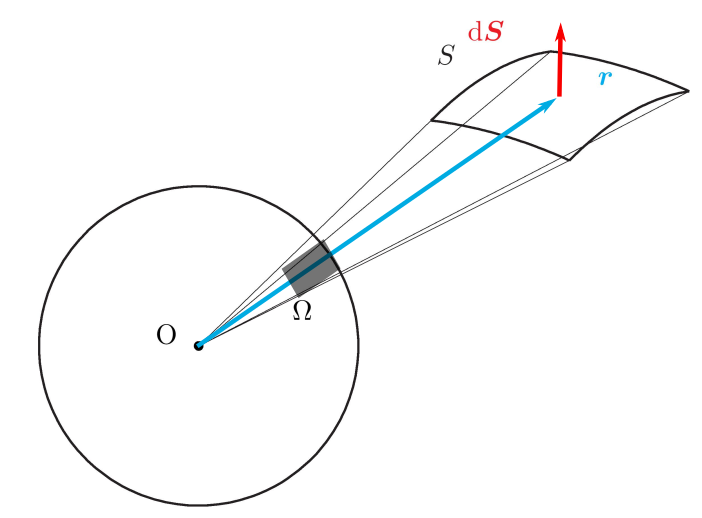
\includegraphics[width=7cm]{picture/steradian}
 \caption{立体角}
\label{fig:steradian}
\end{figure}

問題は,この面積をいかにして求めるかである.
実は,$\Omega$は次のように求めることができる.
\begin{align}
\Omega = \int_S \frac{\bm{r} }{r^3} \cdot \mathrm{d} \bm{S}
\label{eq:ritaikaku}
\end{align}
積分の式を解釈するときには被積分関数を眺めるとよいのであった.
$\bm{r}$と$\mathrm{d}\bm{S}$のなす角を$\theta$とすれば,
\begin{align*}
\frac{\bm{r}}{r^3} \cdot \mathrm{d} \bm{S} = \frac{1}{r^2} \, \mathrm{d} S \cos \theta
\end{align*}
である.
$\mathrm{d}S \cos\theta$という項について考えよう.
そもそも$\mathrm{d}S$というのは,位置$\bm{r}$における$S$の面素であり,
その意味は位置$\bm{r}$のごく近辺において$S$を平面とみなしたときの
その領域の面積であった.
それに$\cos \theta$をかけた量というのは,この領域を真上から角度
$\theta$だけずれた方向,つまり$\bm{r}$方向から眺めたときに
見える領域の面積を表している.
細かいことを考えなければこのことを示すのはあまり難しくはないから読者に任せておくことにしよう.

ここで,$S$を微小領域に分割したとき,各微小領域を$\bm{r}$方向から眺めた時に見える領域と
Oからその微小領域のふちに向かう各半直線と球面の交点として得られる領域
(図\ref{fig:steradian}の陰になっている部分)
は相似であって,その相似比は$1 : r$である.従ってその面積比は$1 : r^2$である.
よって,面積$\mathrm{d}S$の微小領域がつくる立体角$\mathrm{d} \Omega$は
\begin{align}
\mathrm{d} \Omega = \frac{1}{r^2} \, \mathrm{d} S \cos \theta
= \frac{\bm{r}}{r^3} \cdot \mathrm{d} \bm{S} 
\label{eq:bisyouomega}
\end{align}
となる.これを$S$全体にわたって足し合わせれば式(\ref{eq:ritaikaku})が得られることになる.

立体角の角度の単位はラジアンにならって
\emph{ステラジアン}\index[widx]{すてらじあん@ステラジアン}$[\mathrm{sr}]$
という単位が使われている.これもやはり無次元量である.

半径1の球面の表面積は$4 \pi$であるから,
任意の閉曲面$S_0$について,Oが$S_0$内部にある場合,
$S_0$のOに関する立体角は$4 \pi$ということになる.
しかしこれを式(\ref{eq:ritaikaku})に基づいて計算するのは少し面倒である.
また,Oが$S_0$外部にある場合,$S_0$のOに関する立体角は0になる.
これも式(\ref{eq:ritaikaku})に基づいて計算することはできるのだが,
ちょっと面倒なので本書では省略させてもらうことにする.


\section{微分演算子$\nabla$について}
電磁気学を学んでいるとよくこんなのが出てくる.
\begin{align}
\nabla = \left[
 \begin{array}{c}
\displaystyle
\frac{\partial}{\partial x} \\
\displaystyle
\frac{\partial}{\partial y} \\
\displaystyle
\frac{\partial}{\partial z} 
 \end{array}
\right] 
= \bm{e}_x \frac{\partial}{\partial x} + \bm{e}_y \frac{\partial}{\partial y} 
+ \bm{e}_z \frac{\partial}{\partial z}
\label{eq:nabla}
\end{align}
この記号$\nabla$は\emph{ナブラ}\index[widx]{なぶら@ナブラ($\nabla$)}と読む.
$\nabla$はベクトルとは言えないが,ベクトルっぽいものである.
よって手書きでは線を一本追加して二重文字で書く.
$\nabla$は微分演算子の一種であるとよく言われる.
$\nabla$は初学者キラーといっても過言ではないだろう.多くの人がこいつに苦しめられてきたにちがいない.
かくいう私もその1人である.だが,$\nabla$というのは単体ではまったく意味をなさない.
この記号を用いることで多くの式が簡便に,かつ統一的に表現できて便利だから使っているにすぎないのだ.
初学者の多くは$\nabla$単体の意味を必死に考え,そして挫折する.
だが,意味をもつのは$\nabla$単体ではなくそれを使って構成される種々の量である.
それを今から考えてみよう.
\subsection{微分演算子とは何か}
$\nabla$について考える前に,``演算子'',そして``微分演算子''というものについて考えてみよう.

それ単体では機能せず,他のものに対して何かしらの計算の指示を与えるものを
\emph{演算子}\index[widx]{えんざんし@演算子|textbf}という.数学者はよく``作用素''と呼んでいる.
``計算の指示''というと堅苦しく聞こえるかもしれないが,$\sin$とか$\ln$とか,
そんな感じのものが演算子である.
$\sin$や$\ln$というのは後ろのモノに対して
その正弦の値や自然対数
\footnote{自然対数というのは底が
Napire数$e$であるような対数のこと.数学では普通$\log$という記号で表すが,
数学以外では$\ln$と表すことが多い.}
の値を計算してくれ,という記号である.
和を表す記号$+$や積を表す記号$\times$も演算子の一種である.
また,演算子の中で後ろの関数を微分してくれ,という指示を含むような演算子のことを
\emph{微分演算子}\index[widx]{えんざんし@演算子!びぶん@微分---}という.
$\displaystyle \frac{\mathrm{d}}{\mathrm{d}x}$
や$\displaystyle \frac{\partial}{\partial x}$などは微分演算子である.

さらに,何かしらのモノに演算子をくっつけて実際に計算をさせることを演算子を\emph{作用させる}
\index[widx]{えんざんし@演算子!をさようさせる@---を作用させる}という.
なんだか偉そうに聞こえるが,大した言葉ではない.日常的にやっていることである.
例えば,数$x$の自然対数をとるという操作は``$x$に対して演算子$\ln$を作用させる''と言い換えることができるし,
$x, \, y$関数$f(x, \, y)$を$x$で偏微分するという操作は``関数$f$に微分演算子
$\displaystyle \frac{\partial}{\partial x}$を作用させる''
と言い換えることができる.言葉を言い換えるだけでなんだかとても高尚なことをやっている気分になる.
演算子というものに対してはそのくらいの気持ちで付き合っていけばいいのだ. 

演算子というものを考えると式を略記できることがある.例えば,
$$
\frac{\partial^2 f}{\partial x^2} + \frac{\partial^2 f}{\partial y^2} + \frac{\partial^2 f}{\partial z^2}
$$
という式があったときに,これは
$$
\left( \frac{\partial^2}{\partial x^2} + \frac{\partial^2}{\partial y^2} + \frac{\partial^2}{\partial z^2} \right) f
$$
と略記できる.この記法は式を簡潔に記述するだけでなく,式に隠れた対称性や規則性を浮き彫りにしてくれることがある.

\subsubsection{演算子は順番に気を付けろ}
使うのにはとっても便利な演算子であるが,
演算子は作用させる順番によって結果が変わることがある.
このことに気を付けないまま計算を進めた結果,なんだかよくわからないものが得られてしまったりするので気を付けなければならない.

例として微分演算子でやってみよう.微分演算子$\displaystyle \frac{\mathrm{d}}{\mathrm{d}x}$と
演算子としての関数$g$があったとする.関数$f$に$g$を作用させる,というのはその積$gf$をとれ
という計算をさせることだと解釈しておく.

まず,関数$f$に$\displaystyle \frac{\mathrm{d}}{\mathrm{d}x}$を作用させてから$g$を作用させてみる.
結果は
$$
g \left( \frac{\mathrm{d}f}{\mathrm{d}x} \right)  = g \frac{\mathrm{d}f}{\mathrm{d}x}
$$
となる.特に変わったところはない.

次に,$g$を作用させてから$\displaystyle \frac{\mathrm{d}}{\mathrm{d}x}$を作用させてみよう.
結果は
$$
\frac{\mathrm{d}}{\mathrm{d}x} (gf) = f \frac{\mathrm{d}g}{\mathrm{d}x} + g \frac{\mathrm{d}f}{\mathrm{d}x}
$$
となり,前者とは違った結果になってしまう.
演算子に関しては交換法則は成り立っていないのである.
座標変換などを考えるときにそういうことに出くわすことがあるだろう.
そのときになったら気を付けてもらえばいい.

\subsection{$\nabla$を使ってみよう}
演算子というのはそれ単体では大した意味を持たないことが多いというのはわかってもらえただろうか.
$\nabla$もそうである.$\nabla$単体の意味をどう解釈してみようか努力してみてもまったくの無駄である.
それよりも,$\nabla$を使って構成される量の方に興味があるのである.
本書ではスカラー場の勾配を表すグラーディエント,ベクトル場の発散を表すダイバージェンス,
そしてベクトル場の回転を表すローテーション(もしくはカール)の3つを学ぶ.

\subsection{スカラー場の勾配}
スカラー場$\phi(x, \, y, \, z)$があったとする.これに$\nabla$を作用させてベクトルを作ってみよう.
\begin{eqnarray}
\nabla \phi = \left[
 \begin{array}{c}
\displaystyle
\frac{\partial \phi}{\partial x} \\
\displaystyle
\frac{\partial \phi}{\partial y} \\
\displaystyle
\frac{\partial \phi}{\partial z} 
 \end{array}
\right]
\label{eq:gradnabla}
\end{eqnarray}
というベクトルができた.このベクトルをスカラー場$\phi$の\emph{勾配}
\index[widx]{すからーば@スカラー場!のこうばい@---の勾配}という.
このベクトルは,各点$(x, \, y, \, z)$に対し,$\phi$が最も急激に増加するような方向を指し示している.
そういうわけで``勾配''などといういかつい名前がついているのである.
と言われても,この式を見せられただけで納得できるような人はまずいない.
しかし,ちょっと考えればすぐにわかるのである.

$\phi$の全微分は
$$
\mathrm{d} \phi = \frac{\partial \phi}{\partial x} \mathrm{d} x 
+ \frac{\partial \phi}{\partial y} \mathrm{d} y +  \frac{\partial \phi}{\partial z} \mathrm{d} z
$$
であった.よく見ると,$\phi$の全微分$\mathrm{d}\phi$は位置の微小変化$\mathrm{d}\bm{r}$と
$\phi$の勾配$\nabla \phi$の内積になっているではないか.
つまり,$\phi$の微小変化$\mathrm{d}\phi$は位置の微小変化$\mathrm{d}\bm{r}$が
$\nabla \phi$の方向を向いているときに最も大きくなるのである.
こうしてみると,``勾配''というネーミングにも納得である.

また,``勾配''は英語ではgradientという.そういうわけで,スカラー場$\phi$の勾配を
\begin{eqnarray}
\mathrm{grad} \, \phi = \left[
 \begin{array}{c}
\displaystyle
\frac{\partial \phi}{\partial x} \\
\displaystyle
\frac{\partial \phi}{\partial y} \\
\displaystyle
\frac{\partial \phi}{\partial z} 
 \end{array}
\right]
\label{eq:gradgrad}
\end{eqnarray}
というように表す流儀もある.好きな方を使えばいいが,どちらの記号が出てきても混乱しないようにはしておくべきだ.

スカラー関数$\phi$について,$\nabla \phi$はベクトル場であった.
このベクトル場$\nabla \phi$を曲線$C$に沿って線積分することを考えよう.
$C$の始点,終点をそれぞれ$\bm{r}_A, \, \bm{r}_B$と表す.
\begin{align*}
\int_C \nabla \phi \cdot \mathrm{d}\bm{s} 
= \int_{\bm{r}_A}^{\bm{r}_B} \mathrm{d} \phi = \phi (\bm{r}_B) - \phi (\bm{r}_A) 
\end{align*}
となる.この計算はあえてノーヒントでいさせてもらおう.ヒントは本書の各所に散らばっている.
ここまできちんと学習を進めてこられたのであれば決して難しくないはずだ.

$\nabla \phi$の線積分は積分経路に依存せず,始点と終点にのみ依存するというわけだ.
すなわち,もしベクトル場$\bm{A}(\bm{r})$を$\bm{A}(\bm{r})=\nabla \phi$
と定めたのであれば,$\bm{A}(\bm{r})$は渦なし場であることがわかる.

\subsection{ベクトル場の発散}
$\nabla$はベクトルっぽいものであった.であれば,ベクトル場$\bm{A}(\bm{r})$について,
$\bm{A}(\bm{r})$と$\nabla$の内積を考えることができるだろう.そしてそれは
\begin{eqnarray}
\nabla \cdot \bm{A} (\bm{r}) =  \frac{\partial A_x}{\partial x} + \frac{\partial A_y}{\partial y} +  \frac{\partial A_z}{\partial z}
\label{eq:divnabla}
\end{eqnarray}
と書き表されるだろう.ベクトル場から1つのスカラーを得た.
これをベクトル場$\bm{A}(\bm{r})$の\emph{発散}\index[widx]{べくとるば@ベクトル場!のはっさん@---の発散}という.
この量は各点$(x, \, y, \, z)$に対し,その地点からベクトル場$\bm{A}(\bm{r})$がどれだけ湧き出しているかを表している.
そういうわけでこの量は発散と呼ばれているのである.全微分と似ているが,ちょっと違う.
微分されているのは$\bm{A}(\bm{r})$自身ではなく,その各成分である.

$x, \, y, \, z$のうち$x$だけが微小量$\mathrm{d}x$だけ変化したとき,$A_x$の微分$\mathrm{d} A_x$は
$$
\mathrm{d} A_x = \frac{\partial A_x}{\partial x} \mathrm{d}x
$$
と表されるのだった.
同様にして,$y$だけが微小量$\mathrm{d}y$だけ変化したとき,$A_y$の微分$\mathrm{d} A_y$は
$$
\mathrm{d} A_y = \frac{\partial A_y}{\partial y} \mathrm{d}y
$$
と表されるし,$z$だけが微小量$\mathrm{d}z$だけ変化したとき,$A_z$の微分$\mathrm{d} A_z$は
$$
\mathrm{d} A_z = \frac{\partial A_z}{\partial z} \mathrm{d}z
$$
と表される.この式に対して疑問がわくようであれば,再度偏微分のところの解説か,常微分の解説に戻っていただきたい.

もし$x$が増加して$A_x$が増加すれば,
それはその場所からベクトル場の$x$成分が湧いて出てきたと考えるほかはない.
``$x$が増加した''を``ある点よりも$x$軸方向に進んだ点を見た''と言い換えてみるとわかりやすいかもしれない.
ほかの成分に関しても同様である.$x$が変化したときに$\bm{A}(\bm{r})$の$y$成分や$z$成分の変化を考えないのは,
たとえ$y$成分や$z$成分が変化したとしても,
それはベクトル場の$y$成分や$z$成分が湧いて出てきたと考えることはできないからである.
各自図を描いて確認してほしい.こういうことには大いに悩むべきである.

式(\ref{eq:divnabla})は各軸方向の発散の総和である.
たとえ$x$軸の方向にベクトル場が湧き出していたとしても,
同じくらい$y$軸方向にベクトル場の吸い込みが発生していたとするならば,
それはベクトル場の発散があるというべきではないだろう.和をとっているのはそういう意味である.

``発散''は英語でdivergenceという.そんなわけで,ベクトル場の発散を$\nabla$を使わずに
\begin{eqnarray}
\mathrm{div} \, \bm{A}(\bm{r}) = \frac{\partial A_x}{\partial x} + \frac{\partial A_y}{\partial y} +  \frac{\partial A_z}{\partial z}
\label{eq:divdiv}
\end{eqnarray}
と表記することもある.これも好きな方を使うといい.
どちらの書き方が使われていてもきちんと読めるようにしておこう.

\subsection{\textrm{Gauss}の定理}
さて,$\mathrm{div} \, \bm{A}(\bm{r})$は各点$(x, \, y, \, z)$におけるベクトル場の発散を表しているのだった.
ところが,ベクトル場の発散といえば閉曲面上でベクトル場を面積分することでも得られたはずだ.

閉曲面上でベクトル場を面積分することで得られたのは,その閉曲面の内側から外側へのベクトル場の発散の合計であった.
一方,$\mathrm{div}\bm{A}(\bm{r})$が表すのは各点$(x, \, y, \, z)$での発散である.
これを閉曲面$S_0$の内部全体にわたって足し合わせれば,$S_0$の内側から外側への発散の合計が得られるはずだ.
積分領域は3次元領域であるから,これを$V$と表記しておこう.
この積分は,$V$を細かいさいころのようなブロックに分割して足し合わせていくイメージである. 
すると,次のような等式が成り立っているはずだ.
\begin{eqnarray}
\int_V \mathrm{div} \, \bm{A}(\bm{r}) \, \mathrm{d}V = \oint_{S_0} \bm{A}(\bm{r}) \cdot \mathrm{d}\bm{S}
\label{eq:Gaussthe}
\end{eqnarray}
ただし,$V$は$S_0$内部全体であり,右辺の面積分の向きは
$S_0$の内部から外部に向かうような向きであるとする.
式(\ref{eq:Gaussthe})を\textbf{Gaussの定理}\index[widx]{Gaussのていり@Gaussの定理}
\index[nidx]{Gauss@Gauss(ガウス)}と呼ぶ.
詳しい導出はやらない.その代わり式の解釈をしておこう.式(\ref{eq:Gaussthe})の両辺をよく眺めてほしい.
左辺の積分領域は$V$,つまり3次元領域で,右辺の積分領域は$S_0$,つまり2次元領域である.
Gaussの定理を利用するときにはこの性質をうまく利用することが多い.
つまり,Gaussの定理は積分領域を変更したいときに使われるのである.
たとえば,Maxwell\index[nidx]{Maxwell@Maxwell(マクスウェル)}
方程式を微分形から積分形,もしくはその逆に変形するときにこの定理は使われる.

とはいえ,いま理解すべきは左辺と右辺がともにベクトル場の発散を表しているということだ.
それさえ納得できてしまえば式(\ref{eq:Gaussthe})を忘れることもないだろう.
\subsection{ベクトル場の回転}
さっきやったのは$\nabla$とベクトルの内積である.今度は$\nabla$とベクトルの外積を考えてみよう.
何も考えずに計算してみれば,このようなベクトルが得られるはずだ.
\begin{eqnarray}
\nabla \times \bm{A}(\bm{r}) = \left[
\begin{array}{c}
\displaystyle
\frac{\partial A_z}{\partial y} - \frac{\partial A_y}{\partial z} \\
\displaystyle
\frac{\partial A_x}{\partial z} - \frac{\partial A_z}{\partial x} \\
\displaystyle
\frac{\partial A_y}{\partial x} - \frac{\partial A_x}{\partial y} 
\end{array}
\right]
\label{eq:rotnabla}
\end{eqnarray}
ベクトルの外積の成分表示のところをじっくり見ながら計算してみてほしい.
ベクトル場からまた違うベクトルを得た.これをベクトル場$\bm{A}(\bm{r})$の
\emph{回転}\index[widx]{べくとるば@ベクトル場!のかいてん@---の回転}という.このベクトルは各点$(x, \, y, \, z)$に対し,
その地点でベクトル場$\bm{A}(\bm{r})$がどの方向にどれだけの渦を巻いているかを表すベクトルである.
このベクトルが``回転''と呼ばれているのはそこからきている.
回転といってもいろいろな方向が考えられるだろう.
ベクトル場の回転がまたベクトルになっているのはそういうことである.
ベクトル場がどの向きに渦を巻いているかをしているかをそのベクトル場の回転の向きで,
渦がどの程度の強さなのかをそのベクトル場の回転のノルムによって表しているのである.

いま何を言っているかよくわからない人は,おそらく力学で回転関係の話を
学んでいないか,もしくはきちんと数学的に定式化された形で学んでいないかのどちらかだろう.
そういう人は多いだろうから,ざっくりとだが復習しておこう.
\subsubsection{回転を1本のベクトルで表す}
1本ベクトルが持っている方向というのは1つである.これはまったく当たり前のことである.
これだけで``回転''を表現するのは不可能に見えるかもしれない.
川の流れがぐるぐると渦を巻いている様子を想像してみると,それぞれの点では流れの向きはばらばらである.
しかし,全体を見てみるとなんとなく渦を巻いている.そんなイメージである.
この川の渦をたった1本のベクトルで表したい.
それにはどうすればよいだろうか? 必要なのは回転軸という考え方である.

ベクトルの外積のところで``2つのベクトル$\bm{a}, \, \bm{b}$について,
その外積$\bm{a} \times \bm{b}$の向きは,$\bm{a}$から$\bm{b}$の向きに右ネジを回したとき,
そのネジが進む方向であると定義する''と説明したのを覚えているだろうか.
あの場面では先にネジが回転する方向がわかり,それをもとに外積の向きが決まったのであった.
そう,回転の向きとベクトルの向きが対応しているのである.

逆に考えることはできないだろうか? ベクトルの向きが回転の方向を決めていると考えるのである.
それには``こういうベクトルにはこういう回転が対応しますよ''という約束事を指定しなくてはならない.
どうせなら外積と同じにしてしまおう.
あるベクトルが表す回転の向きは,そのベクトルの向きが右ネジが進む向きになるような
ネジの回転方向であると約束することにする.
回りくどい言い方だが,要はベクトルの外積のときと同じ対応関係になるようにしたのである.
ベクトルの大きさは,回転の強さを表すことにしておこう.これは自然な考えである.
大きさが大きいベクトルほどそのベクトルが表す回転は激しいのである.

これで1本のベクトルと1つの回転が完全に対応付けられた.
勘違いしてほしくないのだが,これはすべてのベクトルが回転を表すと決めたわけではない.
もしこのベクトルが回転を表すとしたら,それはこういう回転方向と強さを表していますよ,
というように約束事を作っただけである.
力$\bm{F}$が回転を表しているわけなかろう? そんなニュアンスである.

力学においてはこの約束事のもと,回転に関する種々の物理量がベクトル化される.
力のモーメント$\bm{N}$や角速度$\bm{\omega}$などである.
このようにベクトルで表しておくと,いろいろな方向の回転に対して式を統一的に表現できて便利である.
基準点からみて位置$\bm{r}$にある物体に力$\bm{F}$がはたらいているとき,
その力のモーメントは$\bm{N}=\bm{r}\times\bm{F}$と書き表され,
物体の角速度が$\bm{\omega}$であればその速度は$\bm{v}=\bm{\omega}\times\bm{r}$
と書き表される.

もし外積の順序を逆にしてしまうと,ベクトルの向きと回転方向の対応関係が崩れてしまう.
ベクトルの向きと回転方向の向きの対応関係は,人間が式を読み解くときに使うもので,
式そのものの中に回転方向が内蔵されているわけではないのである.
たとえば角速度$\bm{\omega}$がいくら回転を表しているといっても,
$\bm{\omega}$自体はただのベクトルである.
$\bm{\omega}$の向きは回転軸の方向を表していて,$\bm{\omega}$の大きさは回転の激しさを表している.
これが約束した正しい方向の回転を表すように仕向けるためには,
作った公式がうまく自身の方向と回転方向との関係を反映したものでなくてはならない.
角速度$\bm{\omega}$の例でいえば,$\bm{v}=\bm{\omega}\times\bm{r}$という式がそれである.

\begin{itembox}[l]{検討}
いまの話では,回転という現象をたった1本のベクトルで表せることを学んだ.
``回転''と``渦''はほぼ同じ意味だと思ってもらって構わない.
川に渦が巻いている状況を考えよう.渦であるからそれはベクトルで表せるはずだ.
しかし,川の渦は場所によって強さが違う.向きさえ一定ではないだろう.

このような状況では,この川の渦をたった1本の定まったベクトルとして表すのは不可能である.
いったいどうしたらいいだろう?
\end{itembox}

\subsubsection{ベクトル場の回転について考える}
ちょっと(しかし重要な)脱線をしたところで,話を戻そう.ベクトル場の回転というのは次の式で定義されるのだった.
\begin{eqnarray}
\nabla \times \bm{A}(\bm{r}) = \left[
\begin{array}{c}
\displaystyle
\frac{\partial A_z}{\partial y} - \frac{\partial A_y}{\partial z} \\
\displaystyle
\frac{\partial A_x}{\partial z} - \frac{\partial A_z}{\partial x} \\
\displaystyle
\frac{\partial A_y}{\partial x} - \frac{\partial A_x}{\partial y} 
\end{array}
\right]
\label{eq:rotnabla2}
\end{eqnarray}
このベクトルがベクトル場$\bm{A}(\bm{r})$の回転を表しているというのであった.
このことについて,少し考えてみよう.とはいえ,成分が3つあるので,まずは$z$成分から考えてみることにする.
なぜ$z$成分から考えるかというと,$\nabla \times \bm{A}(\bm{r})$の$z$成分が$\bm{A}(\bm{r})$の
$xy$平面内の回転を表しているからである.
このことについて考えてみる.

$\nabla \times \bm{A}(\bm{r})$の$z$成分は
\begin{eqnarray}
(\nabla \times \bm{A}(\bm{r}))_z = \frac{\partial A_y}{\partial x} - \frac{\partial A_x}{\partial y} 
\label{eq:rotnablaz}
\end{eqnarray}
である.ベクトルの成分を表すのに,そのベクトルに対応する成分を表す添え字をつけることがある.
こういう表記は大概予告なしに使われることがあるので覚えておこう.

さて,式(\ref{eq:rotnablaz})が何を表しているのか考えてみよう.
まずは第1項
$$
\frac{\partial A_y}{\partial x}
$$
からである.この項は$x$が変化したときの$\bm{A}(\bm{r})$の$y$成分の変化率を表しているのだった.
もしこの項が正であれば,それは$x$軸の正方向に進めば進むほど$\bm{A}(\bm{r})$の$y$成分が増加していくことになる.

第2項
$$
-\frac{\partial A_x}{\partial y}
$$
についても同じように考えてやる.この項は$y$が変化したときの$\bm{A}(\bm{r})$の$x$成分の変化率を表している.
頭に$-$記号がくっついているので,
この項が全体として正であるときには
$y$軸の正方向に進めば進むほど,$\bm{A}(\bm{r})$の$x$成分が減少していくことになる.

すなわち,$x$に対して$\bm{A}(\bm{r})$の$y$成分が増加し,かつ$y$に対して$\bm{A}(\bm{r})$の$x$成分が減少するとき,
$\nabla \times \bm{A}(\bm{r})$の$z$成分は大きな値をとる.
このような場合,$\bm{A}(r)$の分布はどうなっているだろうか? 図に書き起こしてみよう.
\begin{figure}[h]
 \begin{minipage}{0.5\hsize}
  \begin{center}
   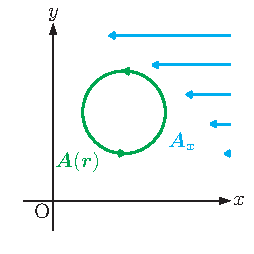
\includegraphics[width=5cm]{picture/vecterana5}
  \end{center}
 \caption{ベクトル場の回転その1}
 \label{fig:vecrot1}
\end{minipage}
\begin{minipage}{0.5\hsize}
  \begin{center}
   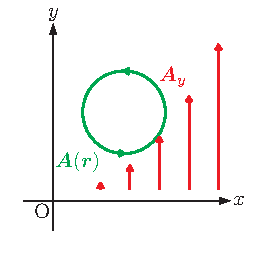
\includegraphics[width=5cm]{picture/vecterana6}
  \end{center}
 \caption{ベクトル場の回転その2}
 \label{fig:vecrot2}
\end{minipage}
\end{figure} \\

$A_x$と$A_y$の分布を見たときに,
$\bm{A}(\bm{r})$の渦のようなものが見えてくる.
$xy$平面を川だと思い,$\bm{A}(\bm{r})$を川の流れを表すベクトル場だと思ってみる.
そして,この川の緑色の円の中心あたりに水車があると思ってみよう.
水車は図の緑の矢印のような向きに回転するはずだ.


$xy$平面に反時計回りの渦が発生しているとき,これを右ネジが回転する方向だと思うことにすると,
右ネジは$z$軸正方向を進むことになる.
したがって,この渦を表すベクトルは$z$軸正方向を向いているべきである.
また,図を見る限り,$A_x$と$A_y$の変化が激しいほど強い渦が発生していることになるだろう.
これらのことから察するに,この渦を表しているのは$\nabla \times \bm{A}(\bm{r})$の$z$成分である.
すなわち,$\nabla \times \bm{A}(\bm{r})$の$z$成分は
ベクトル場$\bm{A}(\bm{r})$の$xy$平面上にある渦の向きと強さを表しているのである.
もしも$\nabla \times \bm{A}(\bm{r})$の$z$成分が負であれば,
それはベクトル場$\bm{A}(\bm{r})$の$xy$平面上にある渦の向きが
図と逆向きであるということだ.

と書いてみたものの,
これは$\nabla \times \bm{A}(\bm{r})$が$\bm{A}(\bm{r})$の回転を表していることを無理やりにでも納得してもらうための
都合のいい例を出したにすぎない.
実際のベクトル場はもっと複雑で,どう見ても渦には見えないようなベクトル場であってもそれとナブラとの外積をとってみると
$\bm{0}$にはなってくれないことがしょっちゅうある.そういうときは定義式を眺めてそんなものかと納得しておけばよい.
人間の勝手な思い込みなどさっさと捨て去ってしまうべきだ.
\begin{itembox}[l]{課題}
上の考察にならって,$\nabla \times \bm{A}(\bm{r})$の$x$成分や$y$成分が何を表しているかを調べよ.
\end{itembox}

$\nabla \times \bm{A}(\bm{r})$が$\bm{A}(\bm{r})$の回転を表していることは理解できただろう.
そういうわけで,ベクトル場の回転を英単語rotationやcurlからとって
\begin{eqnarray}
\mathrm{rot} \, \bm{A}(\bm{r}) = \left[
\begin{array}{c}
\displaystyle
\frac{\partial A_z}{\partial y} - \frac{\partial A_y}{\partial z} \\
\displaystyle
\frac{\partial A_x}{\partial z} - \frac{\partial A_z}{\partial x} \\
\displaystyle
\frac{\partial A_y}{\partial x} - \frac{\partial A_x}{\partial y} 
\end{array}
\right]
\label{eq:rotrot}
\end{eqnarray}
だったり,
\begin{eqnarray}
\mathrm{curl} \, \bm{A}(\bm{r}) = \left[
\begin{array}{c}
\displaystyle
\frac{\partial A_z}{\partial y} - \frac{\partial A_y}{\partial z} \\
\displaystyle
\frac{\partial A_x}{\partial z} - \frac{\partial A_z}{\partial x} \\
\displaystyle
\frac{\partial A_y}{\partial x} - \frac{\partial A_x}{\partial y} 
\end{array}
\right]
\label{eq:rotcurl}
\end{eqnarray}
というように表すことがある.rot表記は主に日本で,curl表記は主に海外で用いられることが多いようである.
好きなものを採用すればいいが,やはりどれが出てきても混乱しないようにはしておこう.

\subsection{\textrm{ Stokes}の定理}
$\mathrm{rot} \, \bm{A}(\bm{r})$はベクトル場$\bm{A}(\bm{r})$の回転を表すのだった.
回転を表すといっても,$\mathrm{rot} \, \bm{A}(\bm{r})$はベクトル場で,
$\bm{A}(\bm{r})$の各点$(x, \, y, \, z)$における局所的な回転を表している.
これをある曲面$S$上全体にわたって面積分したらどうなるだろうか? ベクトル場の面積分が表しているのは
ベクトル場がその曲面を垂直に貫くような場の分布であった.
いま積分するのは$\bm{A}(\bm{r})$自身ではなく$\mathrm{rot} \, \bm{A}(\bm{r})$である.
$\mathrm{rot} \, \bm{A}(\bm{r})$が曲面を垂直に貫いているような分布がどれだけあるかを計算するということは,
すなわちもとのベクトル場がその曲面にそってどのくらいの強さの渦を巻いているかを計算しているのと
同じことである.従って,曲面$S$のふちを$C_0$とすれば,$C_0$はもちろん閉曲線で
\begin{eqnarray}
\int_S \mathrm{rot} \, \bm{A}(\bm{r}) \cdot \mathrm{d} \bm{S} =
\oint_{C_0} \bm{A}(\bm{r}) \cdot \mathrm{d}\bm{s}
\label{eq:Stokesthe}
\end{eqnarray}
という式が成り立っているということが推測できる.ただし,$S$は空間にある任意の曲面で,
$C_0$はそのふちである.
ただし,曲面$S$の向きは$C_0$に沿って曲面のふちを1周するとき,
その向きに右ネジを回したときにネジが進むような向きであるとする.

実際,式(\ref{eq:Stokesthe})は厳密に成り立っていて,
\textbf{Stokesの定理}\index[widx]{Stokesのていり@Stokesの定理}
\index[nidx]{Stokes@Stokes(ストークス)}と呼ばれている.
Gaussの定理とよく似た形をした等式である.あちらと合わせて頭に叩き込んでしまおう.

この式もGaussの定理と同じく,線積分を面積分に変換したり,またその逆を行ったりするときによく使われる.
だが,とりあえず今確認すべきなのは,
式(\ref{eq:Stokesthe})の両辺がともに$\bm{A}(\bm{r})$の回転を表しているということである.

\subsection{ベクトル場のポテンシャル}
Gaussの定理やStokesの定理を学んだところで,
どうやらベクトル場の閉じた領域での積分は
そのベクトル場の発散や回転に関係しているらしいというのが見えてきたのであった.
そのあたりについてもう少し詳しく話しておこう.

まずは渦なし場について考えよう.ベクトル場$\bm{A}(\bm{r})$が渦なし場であるというのは,
任意の閉曲線に沿った周回積分が0になるようなベクトル場であった.
渦なし場$\bm{A}(\bm{r})$では$\mathrm{rot} \, \bm{A}(\bm{r}) = \bm{0}$
が常に成り立つ.Stokesの定理とにらめっこしていればすぐにわかるから,
いちいち解説する必要性は感じない.

また,渦なし場に対してはスカラーポテンシャルなる量が定義できるのであった.
以前は渦なし場の線積分としてスカラーポテンシャルを定義したが,
通常``ベクトル場$\bm{A}(\bm{r})$について,$\bm{A}(\bm{r}) = - \nabla \phi (\bm{r})$なる
スカラー関数$\phi(\bm{r})$が存在するとき,この$\phi (\bm{r})$を$\bm{A}(\bm{r})$のスカラーポテンシャルと呼ぶ''
\index[widx]{すからー@スカラー!ぽてんしゃる@---ポテンシャル}
というように定義するのが普通である.
もちろん,この2つの定義はまったく同じ定義であり,
どちらの定義を採用しても構わない.
このことを確認するためのヒントは本書のいたるところに散らばっている.
\begin{itembox}[l]{定理}
ベクトル場$\bm{A}(\bm{r})$について,以下の条件はすべて同値である.
\begin{enumerate}
\item $\mathrm{rot} \, \bm{A}(\bm{r})=\bm{0}$が常に成り立つ.
\item $\bm{A}(\bm{r}) = - \nabla \phi(\bm{r})$なるスカラー関数$\phi(\bm{r})$が存在する.
\item 任意の閉曲線$C_0$に対し,$C_0$に沿った$\bm{A}(\bm{r})$の周回積分が0になる.
\end{enumerate}
\end{itembox}
きちんと証明をしたわけではないが,これまで学んできた事項を整理してやればこうなるのである.
渦なし場については以上のような特徴づけができた.
閉曲線に沿った周回積分と$\mathrm{rot}$,
そしてスカラーポテンシャルは表裏一体の関係にあるのである.

当然次は閉曲面上での面積分と$\mathrm{div}$の関係が気になるところである.
これに関しても同じような特徴づけができることが知られている.
詳しい説明はしないが結果だけ述べておく.
\begin{itembox}[l]{定理}
ベクトル場$\bm{A}(\bm{r})$について,以下の条件はすべて同値である.
\begin{enumerate}
\item $\mathrm{div} \, \bm{A}(\bm{r})=0$が常に成り立つ.
\item $\bm{A}(\bm{r}) = \nabla \times \bm{B} (\bm{r})$なるベクトル場$\bm{B}(\bm{r})$が存在する.
\item 任意の閉曲面$S_0$に対し,$S_0$上での$\bm{A}(\bm{r})$の面積分が0になる.
\end{enumerate}
\end{itembox}
非常に対称的な関係である.ベクトル場$\bm{A}(\bm{r})$について,
$\bm{A}(\bm{r}) = \nabla \times \bm{B}(\bm{r})$なるベクトル場$\bm{B}(\bm{r})$が存在するとき,
この$\bm{B}(\bm{r})$を$\bm{A}(\bm{r})$の\emph{ベクトルポテンシャル}
\index[widx]{べくとる@ベクトル!ぽてんしゃる@---ポテンシャル}と呼ぶ.
スカラーポテンシャルに対してベクトルポテンシャル,実に対称的で美しいネーミングである.

ここまでは発散のないベクトル場,回転(渦)のないベクトル場について考えてきたが,
一般のベクトル場について考えるのであれば,発散も回転もあるのが普通である.
ところが,先に述べた2つの定理を組み合わせたような主張が成り立つことが知られている.
\begin{itembox}[l]{Helmholtzの定理}
ベクトル場$\bm{A}(\bm{r})$について,$\bm{A}(\bm{r})$が無限遠において十分速く$\bm{0}$
に収束するとき,スカラー関数$\phi ( \bm{r})$とベクトル場$\bm{B}(\bm{r})$
が存在して
\begin{align}
\bm{A}(\bm{r}) = - \nabla \phi (\bm{r} ) + \nabla \times \bm{B}(\bm{r})
\label{eq:helmholtz}
\end{align}
が成り立つ.
\end{itembox}
この定理は\textbf{Helmholtzの定理}\index[widx]{Helmholtzのていり@Helmholtzの定理},
\index[nidx]{Helmholtz@Helmholtz(ヘルムホルツ)}
もしくは\emph{ベクトル解析の基本定理}\index[widx]{べくとるかいせきのきほんていり@ベクトル解析の基本定理|see{Helmholtzの定理}}
と呼ばれる非常に重要な定理である.例によって証明はしないが定理の主張は
頭に叩き込んでおきたいものである.

\subsection{ラプラシアン}
ベクトル場の発散と回転は,ベクトルとナブラの内積,および外積を実行することで得られるのであった.
ではナブラ同士ではどうだろうか? 演算子同士を組み合わせて新しい演算子を作り出すというのはよくやることである.
ナブラ同士の外積は結果が美しくならなそうなので内積をやってみよう.
特に何も考えずにやってみると,
\begin{align}
\nabla \cdot \nabla = \frac{\partial^2}{\partial x^2} + \frac{\partial^2}{\partial y^2} + \frac{\partial^2}{\partial z^2}
\label{eq:lap}
\end{align}
とまあなんとなくきれいな感じになる.こういう形の式は物理をやっているといたるところで出てくる.
よく出てくるのだから1文字で表して特別な名前をつけてやろう.
式(\ref{eq:lap})に出てきた演算子を\emph{ラプラシアン}
\index[widx]{らぷらしあん@ラプラシアン($\bigtriangleup$)}と呼び,
記号$\bigtriangleup$で表す.
\begin{align}
\bigtriangleup = \frac{\partial^2}{\partial x^2} + \frac{\partial^2}{\partial y^2} + \frac{\partial^2}{\partial z^2}
\label{eq:Lap}
\end{align}
と定めるのである.式(\ref{eq:lap})を見る限り,ラプラシアンは$\nabla^2$と書いてもいい気がする.
いや,ナブラとそれ自身との内積を求めたのだから$| \nabla |^2$と表すべきだろうか? ただ,
$| \nabla |^2$というのは書くのが面倒だし$\nabla^2$にしておくことにしよう.
今は記号の使い方を定義する場面なのでこういうことができるのだ.式(\ref{eq:lap})を導くのにやった計算は
内積の計算のようなものだが,$\nabla$というのはそもそもベクトルではなくあくまでベクトルっぽいものなのだった.
まとめると,$\bigtriangleup$と$\nabla^2$はまったく同じ意味で,それは式(\ref{eq:Lap})の右辺にある演算子を表している.

なお,$\bigtriangleup$を手書きで書くとき,人によって2重文字にしたりしなかったりする.
ラプラシアンはスカラーっぽいので普通のスカラー量を表すときのようにそのまま三角を書くのも納得である.
しかし,普通に三角で書かれると,もはやギリシャ文字$\Delta$と区別がつかない.
そういうわけで2重文字で書く人もいる.
もっとも,ワープロで打つときもラプラシアンをギリシャ文字$\Delta$で表してしまっていることも多い.
試しにネットで検索してみたらそういうサイトはたくさんあった.
文脈によって書いてある``$\Delta$''がギリシャ文字$\Delta$なのか,
それともラプラシアン$\bigtriangleup$なのかを見分けなくちゃいけないのはなかなか面倒である.
そういうわけで,読者の方々にはラプラシアンは2重文字で書くのを勧めておく.

ラプラシアンはスカラーにでもベクトルにでも作用させることができる.
スカラー関数$\phi$に対しては
\begin{align}
\bigtriangleup \phi = \frac{\partial^2\phi}{\partial x^2} + 
\frac{\partial^2 \phi}{\partial y^2} + \frac{\partial^2 \phi}{\partial z^2}
\label{eqsclap}
\end{align}
というようにラプラシアンを作用させて新しいスカラー関数ができて,ベクトル$\bm{A}$に対しては
\begin{align}
\bigtriangleup \bm{A} = \frac{\partial^2 \bm{A} }{\partial x^2} + 
\frac{\partial^2 \bm{A} }{\partial y^2} + \frac{\partial^2 \bm{A} }{\partial z^2}
\label{eq:veclap}
\end{align}
というようにラプラシアンを作用させて新しいベクトルを作り出すことができる.

$\bigtriangleup \phi$や$\bigtriangleup \bm{A} $がそれぞれ何を表しているかとか,
考えられなくもないが,$\mathrm{div}$や$\mathrm{rot}$のときほど重要な話でもない.
ただなんとなくラプラシアンという演算子があるんだなあとでも思っておけばよいだろう.

注意点として,ラプラシアン$\bigtriangleup$はスカラー関数に作用させる文脈においては演算子$\mathrm{div \, grad}$
とまったく同じ意味を持つが,ラプラシアンをベクトルに作用させる文脈においては$\mathrm{div \, grad}$
と書くべきではない.なぜだかわかるだろうか? スカラー関数$\phi$に対してその勾配$\mathrm{grad} \, \phi$を計算し,
さらにその発散をとるという計算はできるが,これがベクトルになると,
あるベクトル$\bm{A}$の勾配をとるなどという意味不明なことになってしまうからだ.
演算子同士の計算ではこういうことはけっこう起こるので注意しよう.迷ったときには作用させる対象も入れて計算するとよい.

\subsection{微分演算子同士の組み合わせ}
ラプラシアンのときにやったのはナブラとナブラの内積で,これはスカラー関数に作用させるときには
演算子$\mathrm{div \, grad}$と同じ意味を持つのであった.
では,他はどうだろう? 今のところ,$\mathrm{grad, \, div, \, rot}$と3種類ある.
これらをうまいこと組み合わせて何か面白い演算子が作れそうな気がする.
組み合わせのバリエーションは,演算子を作用させる順番によって結果が変わることを考慮すると
$3 \times 3 =9$通りだけありそうだが,実際に試してみると
\begin{align*}
&\mathrm{grad \, div} \\
&\mathrm{div \, grad} \\
&\mathrm{div \, rot} \\
&\mathrm{rot \, grad} \\
&\mathrm{rot \, rot} 
\end{align*}
の5種類しかない.どの演算子が何に作用して何を作るのかを理解していればわかるはずだ.
これをそれぞれ地道に計算してみると,$\mathrm{grad \, div}$に関しては面白い結果は出てこなくて,他のものは
\begin{align}
\mathrm{div \, grad} &= \bigtriangleup \\
\mathrm{div \, rot} &= 0 \\
\mathrm{rot \, grad} &= \bm{0} \\
\mathrm{rot \, rot} &= \mathrm{grad \, div} - \bigtriangleup
\end{align}
という結果になる.ただただ定義に従って地道に計算していくだけなのでいちいち書かなくてもいいだろう.
読者の方々の計算問題としておこう.

\section{微分演算子の座標変換}
微分演算子$\nabla$について学んできたが,
\begin{align*}
\nabla = \bm{e}_x \frac{ \partial}{\partial x} + \bm{e}_y \frac{ \partial}{\partial y}
+ \bm{e}_z \frac{ \partial}{\partial z}
\end{align*}
という書き方はDescartes座標系を基準にして考えていたのであった.
この量を他の座標系で表したいというのが今回のテーマである.
よく使うのが極座標系への変換なので,今回は極座標系への変換を行ってみる.

\subsection{$\nabla$の極座標変換}
さっきの話だけを聞くと,
\begin{align*}
\nabla = \bm{e}_r \frac{ \partial }{\partial r} + \bm{e}_{\theta}
 \frac{ \partial }{\partial \theta } 
 + \bm{e}_{\varphi} \frac{ \partial }{\partial \varphi} 
\end{align*}
と計算して話を終わりにしたくなるが,もちろん間違いである.
あくまで我々が求めたいのはDescartes座標系での$\nabla$を極座標系に変換したいのであって,
極座標系で$\nabla$という演算子を新しく定義したいのではないのである.
つまり,Descartes座標系において関数$f$に$\nabla$を作用させた量
\begin{align*}
\bm{e}_x \frac{ \partial f }{\partial x} + \bm{e}_y \frac{ \partial f } {\partial y}
+ \bm{e}_z \frac{ \partial f }{\partial z}
\end{align*}
が極座標系ではどのような形になるのかを求めたいのである.

そのために何をすべきかといえば,
要は$\bm{e}_x, \, \bm{e}_y, \, \bm{e}_z$と微分演算子を極座標系で表してやればいいのである.
基底ベクトルの方は,以前
\begin{align*}
\bm{e}_x & = & \sin \theta \cos \varphi \, \bm{e} _r & & 
+ \cos \theta \cos \varphi \, \bm{e}_\theta & & - \sin \varphi \, \bm{e}_\varphi & \\
\bm{e}_y & = & \sin \theta \sin \varphi \, \bm{e}_r & & 
+ \cos \theta \sin \varphi \, \bm{e}_\theta & & 
+ \cos \varphi \, \bm{e}_\varphi & \\
\bm{e}_z & = & \cos \theta \, \bm{e}_r & & - \sin \theta \, \bm{e}_\theta &
\end{align*}
という式が成り立つことを懇切丁寧に解説したのだった.
微分演算子の方も以前全微分の解説をしたときに
\begin{align*}
\frac{ \partial f} {\partial r} & 
= \frac{ \partial f} {\partial x} \frac{ \partial x} {\partial r}
+ \frac{ \partial f} {\partial y} \frac{ \partial y} {\partial r}
+ \frac{ \partial f} {\partial z} \frac{ \partial z} {\partial r} \\
\frac{ \partial f} {\partial \theta} & 
= \frac{ \partial f} {\partial x} \frac{ \partial x} {\partial \theta}
+ \frac{ \partial f} {\partial y} \frac{ \partial y} {\partial \theta}
+ \frac{ \partial f} {\partial z} \frac{ \partial z} {\partial \theta} \\
\frac{ \partial f} {\partial \varphi} & 
= \frac{ \partial f} {\partial x} \frac{ \partial x} {\partial \varphi}
+ \frac{ \partial f} {\partial y} \frac{ \partial y} {\partial \varphi}
+ \frac{ \partial f} {\partial z} \frac{ \partial z} {\partial \varphi} \\
\end{align*}
という式が成り立つことを紹介したのであった.
後はこれをいかにも連立方程式っぽく
\begin{align*}
\left[ 
\renewcommand{\arraystretch}{2}
\begin{array}{c}
\dfrac{ \partial f} {\partial r} \\
\dfrac{ \partial f} {\partial \theta} \\
\dfrac{ \partial f} {\partial \varphi}
\end{array}
\right] = \left[
\begin{array}{ccc}
\dfrac{ \partial x} {\partial r} & \dfrac{ \partial y} {\partial r} 
& \dfrac{ \partial z} {\partial r} \\
\dfrac{ \partial x} {\partial \theta} & \dfrac{ \partial y} {\partial \theta} 
& \dfrac{ \partial z} {\partial \theta} \\ 
\dfrac{ \partial x} {\partial \varphi} & \dfrac{ \partial y} {\partial \varphi}
& \dfrac{ \partial z} {\partial \varphi}
\end{array}
\right]
\left[
\begin{array}{c}
\dfrac{ \partial f} {\partial x} \\
\dfrac{ \partial f} {\partial y} \\
\dfrac{ \partial f} {\partial z}
\end{array}
\right]
\end{align*}
と書き表してやる.係数行列の偏微分を実際に求めてやると,
\begin{align*}
\left[ 
\renewcommand{\arraystretch}{2}
\begin{array}{c}
\dfrac{ \partial f} {\partial r} \\
\dfrac{ \partial f} {\partial \theta} \\
\dfrac{ \partial f} {\partial \varphi}
\end{array}
\right] = \left[
\renewcommand{\arraystretch}{1}
\begin{array}{ccc}
\sin \theta \cos \varphi & r \cos \theta \cos \varphi & - r \sin \theta \sin \varphi \\
\sin \theta \sin \varphi & r \cos \theta \sin \varphi & r \sin \theta \cos \varphi \\
\cos \theta & -r \sin \theta & 0
\end{array}
\right]
\left[
\renewcommand{\arraystretch}{2}
\begin{array}{c}
\dfrac{ \partial f} {\partial x} \\
\dfrac{ \partial f} {\partial y} \\
\dfrac{ \partial f} {\partial z}
\end{array}
\right]
\renewcommand{\arraystretch}{1}
\end{align*}
となる.どこかで見たことがあるような式である.あとは
連立方程式を解く要領で
$\dfrac{ \partial f} {\partial x} , \, \dfrac{ \partial f} {\partial y} , \, \dfrac{ \partial f} {\partial z}$
を求めてやればよい.
係数行列がヤコビ行列であることを思い出しつつ,
線形代数学の知識のフル稼働させて係数行列の逆行列を求めてやれば,
\begin{align*}
\left[
\renewcommand{\arraystretch}{2}
\begin{array}{c}
\dfrac{ \partial f} {\partial x} \\
\dfrac{ \partial f} {\partial y} \\
\dfrac{ \partial f} {\partial z}
\end{array}
\right] = \left[
\begin{array}{ccc}
\sin \theta \cos \varphi & \dfrac{ \cos \theta \cos \varphi}{r}
& - \dfrac{ \sin \varphi }{r \sin \theta } \\
\sin \theta \sin \varphi & \dfrac{ \cos \theta \sin \varphi}{r}
& \dfrac{ \cos \varphi }{r \sin \theta } \\
\cos \theta & - \dfrac{ \sin \theta }{r} & 0 
\end{array}
\right] \left[
\begin{array}{c}
\dfrac{ \partial f} {\partial r} \\
\dfrac{ \partial f} {\partial \theta} \\
\dfrac{ \partial f} {\partial \varphi}
\end{array}
\right] 
\end{align*}
となる.つまり,
\begin{align}
\begin{aligned}
\frac{ \partial f}{\partial x} & = & \sin \theta \cos \varphi & \frac{ \partial f}{\partial r}
& + \frac{ \cos \theta \cos \varphi }{r} & \frac{ \partial f}{\partial \theta} 
& - \frac{ \sin \varphi }{ r \sin \theta } &  \frac{ \partial f}{\partial \varphi} \\
\frac{ \partial f}{\partial y} & = & \sin \theta \sin \varphi & \frac{ \partial f}{\partial r}
& + \frac{ \cos \theta \sin \varphi }{r} &  \frac{ \partial f}{\partial \theta} 
& + \frac{ \cos \varphi }{ r \sin \theta } & \frac{ \partial f}{\partial \varphi} \\
\frac{ \partial f}{\partial z} & = & \cos \theta & \frac{ \partial f}{\partial r} 
& - \frac{ \sin \theta }{r} & \frac{ \partial f}{\partial \theta}
\end{aligned}
\label{eq:kyokuDesbibunhenkan}
\end{align}
ということである.関数$f$は任意だったから,結局演算子として
\begin{align}
\begin{aligned}
\frac{ \partial }{\partial x} & = & \sin \theta \cos \varphi & \frac{ \partial }{\partial r}
& + \frac{ \cos \theta \cos \varphi }{r} & \frac{ \partial }{\partial \theta} 
& - \frac{ \sin \varphi }{ r \sin \theta } &  \frac{ \partial }{\partial \varphi} \\
\frac{ \partial }{\partial y} & = & \sin \theta \sin \varphi & \frac{ \partial }{\partial r}
& + \frac{ \cos \theta \sin \varphi }{r} &  \frac{ \partial }{\partial \theta} 
& + \frac{ \cos \varphi }{ r \sin \theta } & \frac{ \partial }{\partial \varphi} \\
\frac{ \partial }{\partial z} & = & \cos \theta & \frac{ \partial }{\partial r} 
& - \frac{ \sin \theta }{r} & \frac{ \partial }{\partial \theta}
\end{aligned}
\label{eq:kyokuDesopehenkan}
\end{align}
という公式が得られたことになる.
演算子的な関係式に書き直したからには
もはや積の順番を勝手に入れ替えることは許されない.
式中にある$\sin \theta \cos \varphi$や$\dfrac{ \cos \varphi}{r \sin \theta}$
も演算子として扱わなければならないのである.

さらに話を進めよう.式(\ref{eq:kyokuDesopehenkan})をちょこっとだけ変形してやって
再度行列形式に書き直してやると
\begin{align}
\left[
\renewcommand{\arraystretch}{2}
\begin{array}{c}
\dfrac{ \partial } {\partial x} \\
\dfrac{ \partial } {\partial y} \\
\dfrac{ \partial } {\partial z}
\end{array}
\right] = \left[
\renewcommand{\arraystretch}{1}
\begin{array}{ccc}
\sin \theta \cos \varphi & \cos \theta \cos \varphi
& - \sin \varphi \\
\sin \theta \sin \varphi & \cos \theta \sin \varphi
& \cos \varphi \\
\cos \theta & - \sin \theta & 0 
\end{array}
\right] \left[
\begin{array}{c}
\dfrac{ \partial } {\partial r} \\
\dfrac{1}{r} \dfrac{ \partial } {\partial \theta} \\
\dfrac{1}{r \sin \theta } \dfrac{ \partial } {\partial \varphi}
\end{array}
\right] 
\label{eq:kyokuDesopehenkan2}
\end{align}
という式が得られる.計算を楽チンに進めるためにちょっとした小細工をしてみる.
我々はどこかでこんな式を見たことがあるとしよう.
\begin{align}
\renewcommand{\arraystretch}{1}
\left[
\begin{array}{ccc}
\bm{e}_x & \bm{e}_y & \bm{e}_z
\end{array}
\right]
= \left[
\begin{array}{ccc}
\bm{e}_r & \bm{e}_\theta & \bm{e}_\varphi 
\end{array}
\right]
\left[
\begin{array}{ccc} 
\sin \theta \cos \varphi & \sin \theta \sin \varphi & \cos \theta \\
\cos \theta \cos \varphi & \cos \theta \sin \varphi & - \sin \theta \\
- \sin \varphi & \cos \varphi & 0
\end{array}
\right]
\label{eq:kyokuDeskiteihenkanx}
\end{align}
行列の成分に共通点が多すぎる.というよりほぼ同じ行列である.
そこで,行列$A$を
\begin{align*}
A = \left[
\renewcommand{\arraystretch}{1}
\begin{array}{ccc} 
\sin \theta \cos \varphi & \sin \theta \sin \varphi & \cos \theta \\
\cos \theta \cos \varphi & \cos \theta \sin \varphi & - \sin \theta \\
- \sin \varphi & \cos \varphi & 0
\end{array}
\right]
\end{align*}
と定めると,式(\ref{eq:kyokuDesopehenkan2})は
$A$の転置行列${}^t \! A$を用いて
\begin{align*}
\left[
\renewcommand{\arraystretch}{2}
\begin{array}{c}
\dfrac{ \partial } {\partial x} \\
\dfrac{ \partial } {\partial y} \\
\dfrac{ \partial } {\partial z}
\end{array}
\right] = {}^t \! A 
\left[
\begin{array}{c}
\dfrac{ \partial } {\partial r} \\
\dfrac{1}{r} \dfrac{ \partial } {\partial \theta} \\
\dfrac{1}{r \sin \theta } \dfrac{ \partial } {\partial \varphi}
\end{array}
\right] 
\end{align*}
と表せて,式(\ref{eq:kyokuDeskiteihenkanx})の方は
\begin{align*}
\renewcommand{\arraystretch}{1}
\left[
\begin{array}{ccc}
\bm{e}_x & \bm{e}_y & \bm{e}_z
\end{array}
\right]
= \left[
\begin{array}{ccc}
\bm{e}_r & \bm{e}_\theta & \bm{e}_\varphi 
\end{array}
\right] A
\end{align*}
と書き換えられることになる.さらに読者が直交行列という言葉も耳にしており,
\begin{align*}
{}^t \! A A = A {}^t \! A = E \quad ( E\text{は単位行列})
\end{align*}
が成り立つことも知っていたとする.
もし知らないのなら線形代数学の教科書を見返してくるか,
とりあえずそのまま受け入れるかして先に進んでほしい.

これらの式を用いれば,$\nabla$が極座標を用いて書き下せて
\begin{align*}
\nabla & = \left[
\renewcommand{\arraystretch}{1}
\begin{array}{ccc}
\bm{e}_x & \bm{e}_y & \bm{e}_z 
\end{array}
\right] \left[
\renewcommand{\arraystretch}{2}
\begin{array}{c}
\dfrac{ \partial } {\partial x} \\
\dfrac{ \partial } {\partial y} \\
\dfrac{ \partial } {\partial z}
\end{array}
\right] \\
& = \left[
\renewcommand{\arraystretch}{1}
\begin{array}{ccc}
\bm{e}_r & \bm{e}_\theta & \bm{e}_\varphi 
\end{array}
\right] A  {}^t \! A 
\left[
\renewcommand{\arraystretch}{2}
\begin{array}{c}
\dfrac{ \partial } {\partial r} \\
\dfrac{1}{r} \dfrac{ \partial } {\partial \theta} \\
\dfrac{1}{r \sin \theta } \dfrac{ \partial } {\partial \varphi}
\end{array}
\right] \\
& = \left[
\renewcommand{\arraystretch}{1}
\begin{array}{ccc}
\bm{e}_r & \bm{e}_\theta & \bm{e}_\varphi 
\end{array}
\right] \left[
\renewcommand{\arraystretch}{2}
\begin{array}{c}
\dfrac{ \partial } {\partial r} \\
\dfrac{1}{r} \dfrac{ \partial } {\partial \theta} \\
\dfrac{1}{r \sin \theta } \dfrac{ \partial } {\partial \varphi}
\end{array}
\right] \\
& = \bm{e}_r \frac{ \partial } {\partial r} 
+ \bm{e}_{\theta} \frac{1}{r} \frac{ \partial } {\partial \theta}
+ \bm{e}_{\varphi} \frac{1}{r \sin \theta } \frac{ \partial } {\partial \varphi}
\end{align*}
となり,結局
\begin{align}
\nabla = \bm{e}_r \frac{ \partial } {\partial r} 
+ \bm{e}_{\theta} \frac{1}{r} \frac{ \partial } {\partial \theta}
+ \bm{e}_{\varphi} \frac{1}{r \sin \theta } \frac{ \partial } {\partial \varphi}
\label{eq:nablakyoku}
\end{align}
という式が得られたことになる.もし関数$f$に$\nabla$を作用させたければ,
\begin{align}
\nabla f = \bm{e}_r \frac{ \partial f } {\partial r} 
+ \bm{e}_{\theta} \frac{1}{r} \frac{ \partial f } {\partial \theta}
+ \bm{e}_{\varphi} \frac{1}{r \sin \theta } \frac{ \partial f } {\partial \varphi}
\label{eq:nablafkyoku}
\end{align}
という計算をすればよいのである.
面倒だった割に結果はシンプルでそこそこ覚えやすい式である.
\begin{itembox}[l]{課題}
2次元Descartes座標系においては,$\nabla$は
\begin{align}
\nabla = \bm{e}_x \frac{ \partial }{\partial x} + \bm{e} _y \frac{\partial}{\partial y}
\label{eq:nabla2d}
\end{align}
と定義される.この定義のもと,先の計算にならい,2次元極座標系における$\nabla$が
\begin{align}
\nabla = \bm{e}_r \frac{\partial }{\partial r} 
+ \bm{e}_{\theta} \frac{1}{r} \frac{\partial}{\partial \theta}
\label{eq:nabla2dkyoku}
\end{align}
と与えられることを示せ.
\end{itembox}

\subsection{発散・回転の極座標変換}
晴れて$\nabla$の極座標系表示を求めることができたわけだが,
満足するにはまだ早い.
極座標を用いて表されたベクトルの発散,回転はどうなるだろう? $\nabla$
とそのベクトルの内積,外積をとってみれば求められそうだが,
具体的にはどう求めたらいいだろう? 極座標系においては
ラプラシアンはどう表されるだろうか? 面倒な計算が続いて嫌になるかもしれないが,
一生に一度だと思って付き合ってほしい.

この後の計算を円滑に進めるために,
$\bm{e}_r, \, \bm{e}_{\theta}, \, \bm{e}_\varphi$の内積,外積の関係を書いておこう.
$\bm{e}_r, \, \bm{e}_{\theta}, \, \bm{e}_\varphi$が互いに直交し,
かつ大きさがすべて1であることを思い出せば
\begin{align}
\begin{aligned}
\bm{e}_r \cdot \bm{e}_r = \bm{e}_\theta \cdot \bm{e}_\theta 
= \bm{e}_\varphi \cdot \bm{e}_\varphi = 1 \\
\bm{e}_r \cdot \bm{e}_\theta = \bm{e}_r \cdot \bm{e}_\varphi 
= \bm{e}_\theta \cdot \bm{e}_\varphi = 0 
\end{aligned}
\label{eq:kyokukiteinaiseki} 
\end{align}
となることや 
\begin{align}
\begin{aligned}
\bm{e}_r \times \bm{e}_\theta & = \bm{e}_\varphi \\
\bm{e}_\theta \times \bm{e}_\varphi & = \bm{e}_r \\
\bm{e}_\varphi \times \bm{e}_r & = \bm{e}_\theta \\
\bm{e}_r \times \bm{e}_r = \bm{e}_\theta \times \bm{e}_\theta
& = \bm{e}_\varphi \times \bm{e}_\varphi = \bm{0}
\end{aligned}
\label{eq:kyokukiteigaiseki}
\end{align}
となることはすぐにわかるはずだ.

準備としてもうひとつ,
$\bm{e}_r, \, \bm{e}_{\theta}, \, \bm{e}_\varphi$
を$r, \, \theta, \, \varphi$で偏微分したものを求めておこう.
$\bm{e}_r, \, \bm{e}_{\theta}, \, \bm{e}_\varphi$は
場所によって異なるベクトルを表すということを思い出してほしい.
$\bm{e}_r, \, \bm{e}_{\theta}, \, \bm{e}_\varphi$をDesartes座標系で表した式を思い出し,
偏微分を実行すれば以下の式が得られるはずだ.

\begin{align}
\begin{aligned}
\frac{\partial}{\partial r } \bm{e}_r = 0 
\, , \; \frac{\partial}{\partial \theta} \bm{e}_r = \bm{e}_\theta 
\, , \; \frac{\partial}{\partial \varphi} \bm{e}_r = \sin \theta \, \bm{e}_\varphi \\
\frac{\partial}{\partial r} \bm{e}_\theta = 0 
\, , \; \frac{\partial}{\partial \theta} \bm{e}_\theta = - \bm{e}_r 
\, , \; \frac{\partial}{\partial \varphi} \bm{e}_\theta = \cos \theta \, \bm{e}_\varphi \\
\frac{\partial}{\partial r} \bm{e}_\varphi = 0 
\, , \; \frac{\partial}{\partial \theta} \bm{e}_\varphi = 0
\, , \; \frac{\partial}{\partial \varphi} \bm{e}_\varphi 
= - \sin \theta \, \bm{e}_r - \cos \theta \, \bm{e}_\theta
 \end{aligned}
 \label{eq:kyokukiteibibun}
 \end{align}
この式について逐一解説する必要はないだろう.
もしわからないのであればそれは今までの内容がきちんと理解できていないということである.
もしそうなら再度確認してきてほしい.

本題に入ろう.ベクトル場$\bm{A}(\bm{r})$があり,$\bm{A}(\bm{r})$が
$\bm{e}_r , \, \bm{e}_{\theta}, \, \bm{e}_{\varphi}$の線形結合として
\begin{align}
\bm{A}(\bm{r}) = A_r \bm{e}_r + A_\theta \bm{e}_\theta + A_\varphi \bm{e}_\varphi
\label{eq:vecseibunkyoku}
\end{align}
というように成分表示されているとする.
$A_r, \, A_\theta, \, A_\varphi$は$\bm{A}(\bm{r})$をDescartes座標系で
\begin{align}
\bm{A}(\bm{r}) = A_x \bm{e}_x + A_y \bm{e}_y + A_z \bm{e}_z 
\label{eq:vecseibunDes}
\end{align}
と成分表示したときの$A_x, \, A_y, \, A_z$と同じであるとは限らず,
それどころか各点$(r, \, \theta, \, \varphi)$によって
異なる値をとることすらあるということに注意しておいてもらいたい.

$\bm{A}(\bm{r})$の発散を求めてみよう.
それには式(\ref{eq:nablakyoku})を用いて
\begin{align*}
\nabla \cdot \bm{A}(\bm{r}) = \left(
\bm{e}_r \frac{ \partial } {\partial r} 
+ \bm{e}_{\theta} \frac{1}{r} \frac{ \partial } {\partial \theta}
+ \bm{e}_{\varphi} \frac{1}{r \sin \theta } \frac{ \partial } {\partial \varphi} \right)
\cdot ( A_r \bm{e}_r + A_\theta \bm{e}_\theta + A_\varphi \bm{e}_\varphi )
\end{align*}
という計算をしてやれば良いと思われるが,このあたりで手が止まる.
といってもこの辺で手を止められるのはきちんと学習できている証なので安心してほしい.
どう計算を進めたらいいだろう.とりあえず展開して
\begin{align*}
\nabla \cdot \bm{A}(\bm{r}) & = 
\bm{e}_r \frac{ \partial } {\partial r} \cdot 
( A_r \bm{e}_r + A_\theta \bm{e}_\theta + A_\varphi \bm{e}_\varphi ) \\
& \hspace{0.5cm} + 
 \bm{e}_{\theta} \frac{1}{r} \frac{ \partial } {\partial \theta} \cdot
 ( A_r \bm{e}_r + A_\theta \bm{e}_\theta + A_\varphi \bm{e}_\varphi ) \\
& \hspace{1cm} + 
 \bm{e}_{\varphi} \frac{1}{r \sin \theta } \frac{ \partial } {\partial \varphi}
 \cdot ( A_r \bm{e}_r + A_\theta \bm{e}_\theta + A_\varphi \bm{e}_\varphi )
\end{align*}
と計算するくらいは許されるだろう.

第1項
\begin{align*}
\bm{e}_r \frac{ \partial } {\partial r} \cdot 
( A_r \bm{e}_r + A_\theta \bm{e}_\theta + A_\varphi \bm{e}_\varphi )
\end{align*}
について考えてみよう.悩むべきは
\begin{align*}
\bm{e}_r \frac{ \partial } {\partial r} \cdot
\end{align*}
がどんな演算を表すかということである.
$\bm{e}_r \dfrac{ \partial }{\partial r}$というのはベクトルのようでただの演算子であった.
その意味は後にくるものを$r$で偏微分し,その後に$\bm{e}_r$を``かけなさい''というように解釈できる.
とすると,「$\cdot$」の存在も加味すれば,$\bm{e}_r \dfrac{ \partial } {\partial r} \cdot$
という演算子は``後にくるベクトルを$r$で偏微分し,
得られたベクトルと$\bm{e}_r$の内積をとりなさい''という意味だと解釈するのが妥当である.

詳しくは解説しないが,ベクトル$\bm{A}(t)$とスカラー関数$f(t)$について
\begin{align}
\frac{ \mathrm{d} } { \mathrm{d} t} ( f(t) \bm{A}(t) ) 
=\frac{ \mathrm{d} f } { \mathrm{d} t} \bm{A} (t)
+ f(t) \frac{ \mathrm{d} \bm{A} } { \mathrm{d} t} 
\label{eq:vecsukarabibun}
\end{align}
という公式が成り立っている.もちろん偏微分についても同じような公式が使える.

式(\ref{eq:vecsukarabibun})とさっきの考察から
\begin{align*}
\bm{e}_r \frac{ \partial } {\partial r} \cdot (A_r \bm{e}_r)
& = \bm{e}_r \cdot \left( \frac{ \partial } {\partial r}  (A_r \bm{e}_r) \right) \\
& = \bm{e}_r \cdot \left( \frac{ \partial A_r} {\partial r} \bm{e}_r 
+ A_r \frac{ \partial \bm{e}_r} {\partial r} \right) \\
& = \bm{e}_r \cdot \left( \frac{ \partial A_r} {\partial r} \bm{e}_r + \bm{0} \right) \\
& = \frac{ \partial A_r} {\partial r} ( \bm{e}_r \cdot \bm{e}_r ) \\
& = \frac{ \partial A_r} {\partial r} \, , \\
\bm{e}_r \frac{ \partial } {\partial r} \cdot (A_\theta \bm{e}_\theta) 
& = \bm{e}_r \cdot \left( \frac{ \partial } {\partial r}  (A_\theta \bm{e}_\theta) \right) \\
& = \bm{e}_r \cdot \left( \frac{ \partial A_\theta} {\partial r} \bm{e}_\theta 
+ A_\theta \frac{ \partial \bm{e}_\theta} {\partial r} \right) \\
& = \frac{ \partial A_\theta} {\partial r} ( \bm{e}_r \cdot \bm{e}_\theta) \\
& = 0 \, , \\
\bm{e}_r \frac{ \partial } {\partial r} \cdot (A_\varphi \bm{e}_\varphi) 
& = \bm{e}_r \cdot \left( \frac{ \partial } {\partial r}  (A_\varphi \bm{e}_\varphi) \right) \\
& = \bm{e}_r \cdot \left( \frac{ \partial A_\varphi} {\partial r} \bm{e}_\varphi 
+ A_\varphi \frac{ \partial \bm{e}_\varphi} {\partial r} \right) \\
& = \frac{ \partial A_\varphi} {\partial r} ( \bm{e}_r \cdot \bm{e}_\varphi) \\
& = 0
\end{align*}
となって,結局のところ
\begin{align*}
\bm{e}_r \frac{ \partial } {\partial r} \cdot 
( A_r \bm{e}_r + A_\theta \bm{e}_\theta + A_\varphi \bm{e}_\varphi )
& = \bm{e}_r \frac{ \partial } {\partial r} \cdot 
( A_r \bm{e}_r + A_\theta \bm{e}_\theta + A_\varphi \bm{e}_\varphi ) \\
& = \bm{e}_r \frac{ \partial } {\partial r} \cdot ( A_r \bm{e}_r ) 
+ \bm{e}_r \frac{ \partial } {\partial r} \cdot ( A_\theta \bm{e}_\theta) \\
& \hspace{2cm}
+ \bm{e}_r \frac{ \partial } {\partial r} \cdot ( A_\varphi \bm{e}_\varphi) \\
& = \frac{ \partial A_r} {\partial r} 
\end{align*}
となることがわかった.

第2項,第3項も同じように計算してやれば良い.
第2項
\begin{align*}
\bm{e}_{\theta} \frac{1}{r} \frac{ \partial } {\partial \theta} \cdot
 ( A_r \bm{e}_r + A_\theta \bm{e}_\theta + A_\varphi \bm{e}_\varphi )
 \end{align*}
 も同じようにばらして計算すると,
\begin{align*}
\bm{e}_{\theta} \frac{1}{r} \frac{ \partial } {\partial \theta} \cdot
( A_r \bm{e}_r ) 
& = \bm{e}_{\theta} \cdot 
\left( \frac{1}{r} \frac{ \partial } {\partial \theta} ( A_r \bm{e}_r )  \right) \\
& =  \bm{e}_{\theta} \cdot 
\left( \frac{1}{r} \frac{ \partial A_r} {\partial \theta} \bm{e}_r
+ \frac{A_r}{r} \frac{ \partial \bm{e}_r} {\partial \theta} \right) \\
& = \frac{1}{r} \frac{ \partial A_r} {\partial \theta} ( \bm{e}_\theta \cdot \bm{e}_r )
+ \frac{A_r}{r} ( \bm{e}_\theta \cdot \bm{e}_\theta ) \\
& = \frac{A_r}{r} \, , \\
\bm{e}_{\theta} \frac{1}{r} \frac{ \partial } {\partial \theta} \cdot
( A_\theta \bm{e}_\theta ) 
& = \bm{e}_{\theta} \cdot 
\left( \frac{1}{r} \frac{ \partial } {\partial \theta} ( A_\theta \bm{e}_\theta )  \right) \\
& =  \bm{e}_{\theta} \cdot 
\left( \frac{1}{r} \frac{ \partial A_\theta} {\partial \theta} \bm{e}_\theta
+ \frac{A_\theta}{r} \frac{ \partial \bm{e}_\theta} {\partial \theta} \right) \\
& = \frac{1}{r} \frac{ \partial A_\theta} {\partial \theta} (\bm{e}_\theta \cdot \bm{e}_\theta)
+ \frac{A_\theta}{r} ( \bm{e}_\theta \cdot ( - \bm{e}_r )) \\
& = \frac{1}{r} \frac{ \partial A_\theta} {\partial \theta}  \, , \\
\bm{e}_{\theta} \frac{1}{r} \frac{ \partial } {\partial \theta} \cdot
( A_\varphi \bm{e}_\varphi ) & = \text{(中略)} = 0 
\end{align*}
となり,結果として
\begin{align*}
\bm{e}_{\theta} \frac{1}{r} \frac{ \partial } {\partial \theta} \cdot
 ( A_r \bm{e}_r + A_\theta \bm{e}_\theta + A_\varphi \bm{e}_\varphi )
 = \frac{A_r}{r} + \frac{1}{r} \frac{ \partial A_\theta} {\partial \theta}
\end{align*}
を得る.
第3項も同じように計算できて,結果だけ書くと
\begin{align*}
 \bm{e}_{\varphi} \frac{1}{r \sin \theta } \frac{ \partial } {\partial \varphi}
 \cdot ( A_r \bm{e}_r + A_\theta \bm{e}_\theta + A_\varphi \bm{e}_\varphi )
 = \frac{ A_r}{r} + \frac{\cos \theta}{r \sin \theta} A_\theta 
 + \frac{1}{r \sin \theta} \frac{ \partial A_\varphi}{\partial \varphi}
 \end{align*}
となる.以上の結果から
\begin{align*}
\nabla \cdot \bm{A}(\bm{r}) & = \frac{ \partial A_r}{\partial r}
+ \frac{A_r}{r} + \frac{1}{r} \frac{ \partial A_\theta} {\partial \theta}
+ \frac{ A_r}{r} + \frac{\cos \theta}{r \sin \theta} A_\theta 
+ \frac{1}{r \sin \theta} \frac{ \partial A_\varphi}{\partial \varphi} \\
& = \frac{ \partial A_r}{\partial r} +  \frac{ 2 A_r}{r}
+ \frac{1}{r} \frac{ \partial A_\theta} {\partial \theta}
+ \frac{\cos \theta}{r \sin \theta} A_\theta 
+ \frac{1}{r \sin \theta} \frac{ \partial A_\varphi}{\partial \varphi}
\end{align*}
となることがわかる.
なんだか汚い式だが,積の微分公式を駆使するともう少しだけまとめることができて,
\begin{align}
\nabla \cdot \bm{A}(\bm{r}) = \frac{1}{r^2}
\frac{ \partial }{\partial r} ( r^2 A_r) + \frac{1}{r \sin \theta} 
\frac{ \partial }{\partial \theta} ( \sin \theta A_\theta)
+ \frac{1}{r \sin \theta} \frac{ \partial A_\varphi} {\partial \varphi}
\label{eq:divkyoku}
\end{align}
となる.何をやったかよく観察してほしい.
こんな計算は二度とやりたくないものである.

ベクトル場の回転の極座標変換も同じように行える.
内積の部分が外積に変わるだけで,2つのベクトル$\bm{A}(t), \, \bm{B}(t)$に対して,
\begin{align}
\frac{\mathrm{d}}{\mathrm{d}t} ( \bm{A} \times \bm{B} )
= \bm{A} \times \frac{\mathrm{d} \bm{B} }{\mathrm{d}t}
+ \frac{ \mathrm{d} \bm{A} } {\mathrm{d}t } \times \bm{B}
\label{eq:gaisekibibun}
\end{align}
が成り立つということをとりあえず受け入れ,発散のときと同じように計算すれば,
\begin{align}
\begin{aligned}
\nabla \times \bm{A} & ( \bm{r} ) 
= \frac{1}{r \sin \theta} \left( \frac{ \partial }{\partial \theta} ( \sin \theta A_\varphi) 
- \frac{\partial A_\theta}{\partial \varphi} \right) \bm{e}_r \\
& + \frac{1}{r} \left( \frac{1}{\sin \theta } \frac{\partial A_r}{\partial \varphi}
- \frac{ \partial }{\partial r}(rA_\varphi) \right) \bm{e}_\theta 
+ \frac{1}{r} \left( \frac{ \partial }{\partial r} ( r A_\theta) 
- \frac{\partial A_r}{\partial \theta} \right) \bm{e}_\varphi
\label{eq:rotkyoku}
\end{aligned}
\end{align}
という結果が得られるはずだ.
もう見るだけで嫌になりそうな式である.

\subsection{ラプラシアンの極座標変換}
さて,残りはラプラシアンである.
とはいえ,やることはさっきまでのものとほとんど変わらない.
関数$f$にラプラシアン$\bigtriangleup$を作用させるというのは
\begin{align*}
\bigtriangleup f = \nabla \cdot ( \nabla f)
\end{align*}
という計算をせよということであった.
極座標系で勾配をとる方法も発散をとる方法もわかっているのだからそれを使って,
\begin{align*}
\begin{aligned}
\bigtriangleup f & = \left(
\bm{e}_r \frac{ \partial } {\partial r} 
+ \bm{e}_{\theta} \frac{1}{r} \frac{ \partial } {\partial \theta}
+ \bm{e}_{\varphi} \frac{1}{r \sin \theta } \frac{ \partial } {\partial \varphi}
\right) \\ 
& \hspace{1cm} \cdot 
\left(
\bm{e}_r \frac{ \partial f } {\partial r} 
+ \bm{e}_{\theta} \frac{1}{r} \frac{ \partial f } {\partial \theta}
+ \bm{e}_{\varphi} \frac{1}{r \sin \theta } \frac{ \partial f } {\partial \varphi}
\right)
\end{aligned}
\end{align*}
という計算をすれば良いのである.
ひたすらちまちま計算していけば,
\begin{align}
\bigtriangleup f = \frac{1}{r^2} \frac{ \partial }{\partial r}
\left( r^2 \frac{\partial f }{\partial r } \right) + \frac{1}{r^2 \sin \theta}
\frac{ \partial }{\partial \theta} 
\left( \sin \theta \frac{ \partial f}{\partial \theta}\right)
+ \frac{1}{r^2 \sin^2 \theta} \frac{ \partial^2 f} { \partial \varphi^2} 
\label{eq:lapkyokuf}
\end{align}
という式が得られるはずである.
よって,演算子としては
\begin{align}
\bigtriangleup = \frac{1}{r^2} \frac{ \partial }{\partial r}
\left( r^2 \frac{\partial }{\partial r } \right) + \frac{1}{r^2 \sin \theta}
\frac{ \partial }{\partial \theta} 
\left( \sin \theta \frac{ \partial }{\partial \theta}\right)
+ \frac{1}{r^2 \sin^2 \theta} \frac{ \partial^2 } { \partial \varphi^2} 
\label{eq:lapkyoku}
\end{align}
という式が成り立っていることがわかる.計算はとても面倒である.

\begin{itembox}[l]{課題}
人生に一度,今がその時である.
極座標変換の定義から始まり,$\nabla$,発散,回転,ラプラシアンに続く
一連の議論の流れを再現し, $\nabla$,発散,回転,ラプラシアン
の極座標変換を省略した計算を含めて導出せよ.
\end{itembox}









